\chapter{Analysis strategy and background estimation}\label{chap:analysis}
\minitoc
Processes producing SUSY particles have significantly smaller cross sections than most SM processes. Therefore, a sophisticated understanding of the relevant production and decay scenarios is needed in order to separate the potential interesting events from the huge amount of SM background. Since this search is targeting SUSY scenarios with bino- and wino-like NLSPs, final states with photons and Z bosons are expected. Choosing the dileptonic decay of the Z boson, there are not many SM background processes leading to the investigated final state. Especially the additional requirement of a photon and $\ptmiss$ in the events reduces most of the background, such that, \eg, the QCD background becomes negligible. Left over are processes producing two same-flavor opposite-charge (SFOC) leptons, one photon and missing transverse momentum. The most important ones are $\ttbar(\PGg)$ production, the combination of Drell-Yan $\PZ/\PGg^{*}$ and $\PZ\PGg$ production, called  Drell-Yan/$\PZ(\PGg)$ from now on, $\PZ\PZ$, and $\PW\PZ$ diboson production. This will be discussed in more detail in \refSec{sec:BKG}.\\
The key strategy of this analysis is to impose as little requirements as necessary, to obtain an event selection, so that many model scenarios can be investigated. Hence, only the existence of all expected final state particles is required, where the Z boson is reconstructed from the two selected leptons. Therefore, loose requirements on the lepton and photon energies can be imposed. Not many additional requirements are needed in the following to obtain a sensitive signal region selection.
% \\
% In the final selection a counting experiment is performed, where predicted and observed data yields are compared, and the result is interpreted in different signal models.

\section{Event Selection}
In this section, the event selection is discussed, including region definitions important for the background prediction, which is based on simulation. In those control regions, each enriched with a specific type of background events and suppressed signal contribution, the simulation is tuned to match the measured data. In an additional validation region, the background prediction will be examined, and finally a two bin counting experiment is performed in the signal region.
\subsection{Preselection}
The preselection acts as a first rough definition of the phase space that is of interest, and rejects inefficient parts of the used triggers. The preselection imposed on the dilepton triggered events is defined as follows:
\begin{itemize}
 \item exactly one SFOC lepton pair ($\Pe\Pe$ or $\PGm\PGm$) as defined in \refSec{sec:reco},
 \item $\pt>25\GeV$ for the leading lepton,
 \item $\pt>20\GeV$ for the trailing lepton,
 \item at least one photon,
 \item $\Delta R(\ell_1,\PGg)>0.3$ and $\Delta R(\ell_2,\PGg)>0.3$,
 \item $81\GeV<m_{\ell\ell}<101\GeV$.
\end{itemize}
The first four conditions imply the existence of the final state particles, including the definition of the physics objects and lepton pair selection explained above, and the $\pt$ requirements determined in the trigger efficiency measurement. The fifth requirement reduces contributions of FSR photons. The invariant dilepton mass requirement ensures that only lepton pairs are selected, that originate from an on-shell Z boson decay, and reduces different contributions of SM backgrounds.
\subsection{Signal region}\label{sec:SRSelection}
The signal region (SR) selection is optimized to maintain high sensitivity for various SUSY scenarios both with electroweak and strong production.
It is defined by the following criteria:
\begin{itemize}
 \item $\ptmiss>150\GeV$,
 \item $\mtTwo>100\GeV$.
\end{itemize}
In the considered models, see \refSec{sec:SMS}, the NLSP can decay to a Z boson or a photon in combination with gravitinos $\gravitino$, which are undetectable and create missing transverse momentum in the event. Therefore, requiring $\ptmiss$ to be larger in the selected events than in most of the SM background processes enables a good separation between SM background and SUSY signal. The $\ptmiss$ threshold is not supposed to be too high, in order to maintain sensitivity to low neutralino masses as well.
Additional high separation power is given by the stransverse mass $\mtTwo$, because it yields a good estimate of the NLSP mass, which is larger than the mass of SM particles. Also, there is no known SM particle which can decay into photons or a Z boson accompanied with neutrinos creating an momentum imbalance in the detector. Therefore, $\mtTwo$ on average is much larger for SUSY processes than for SM processes. Both the $\mtTwo$ and $\ptmiss$ distributions of events fulfilling the preselection are shown in \refFig{fig:SRvariables} for the total background and signal points of each model.
\begin{figure}[tbp]
 \centering
 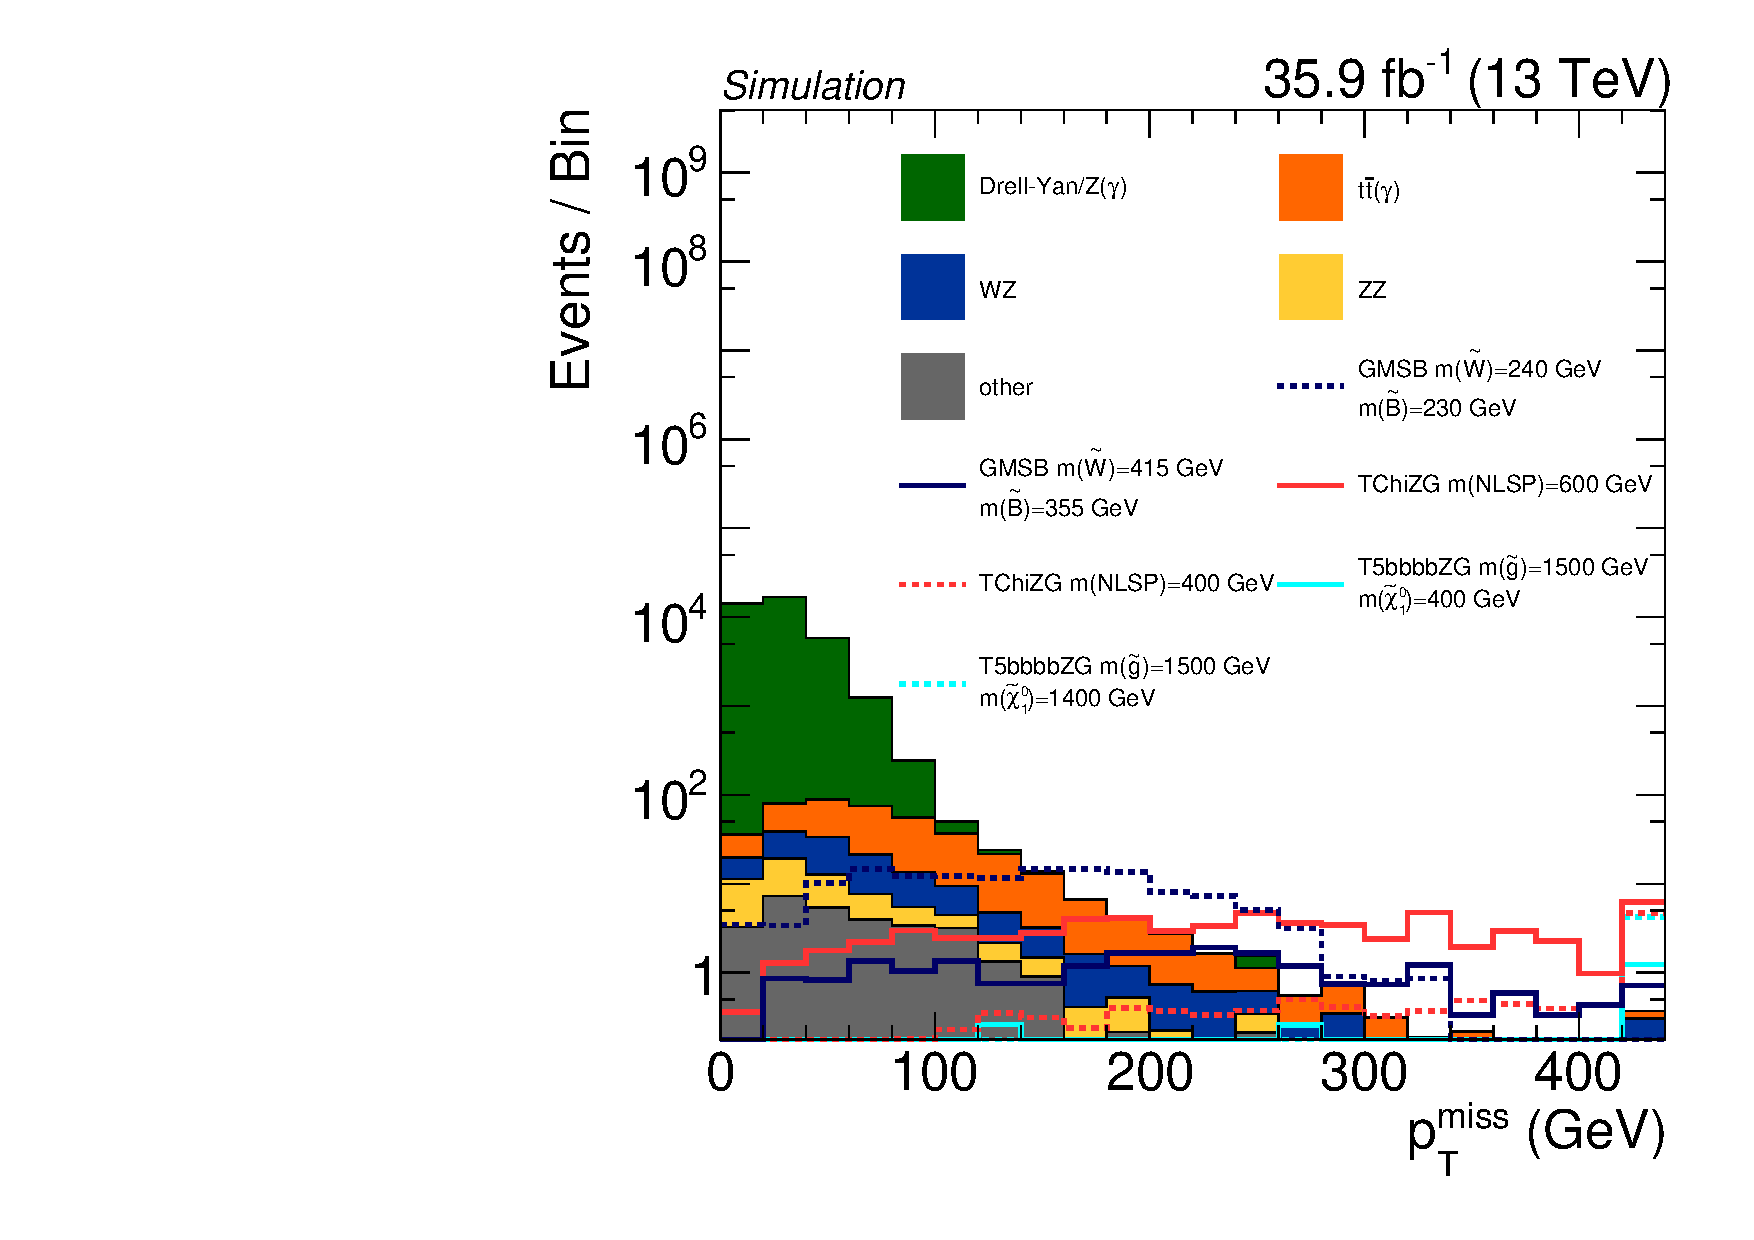
\includegraphics[width=\pairwidth]{figures/plots/onZ_LL_met_log}
 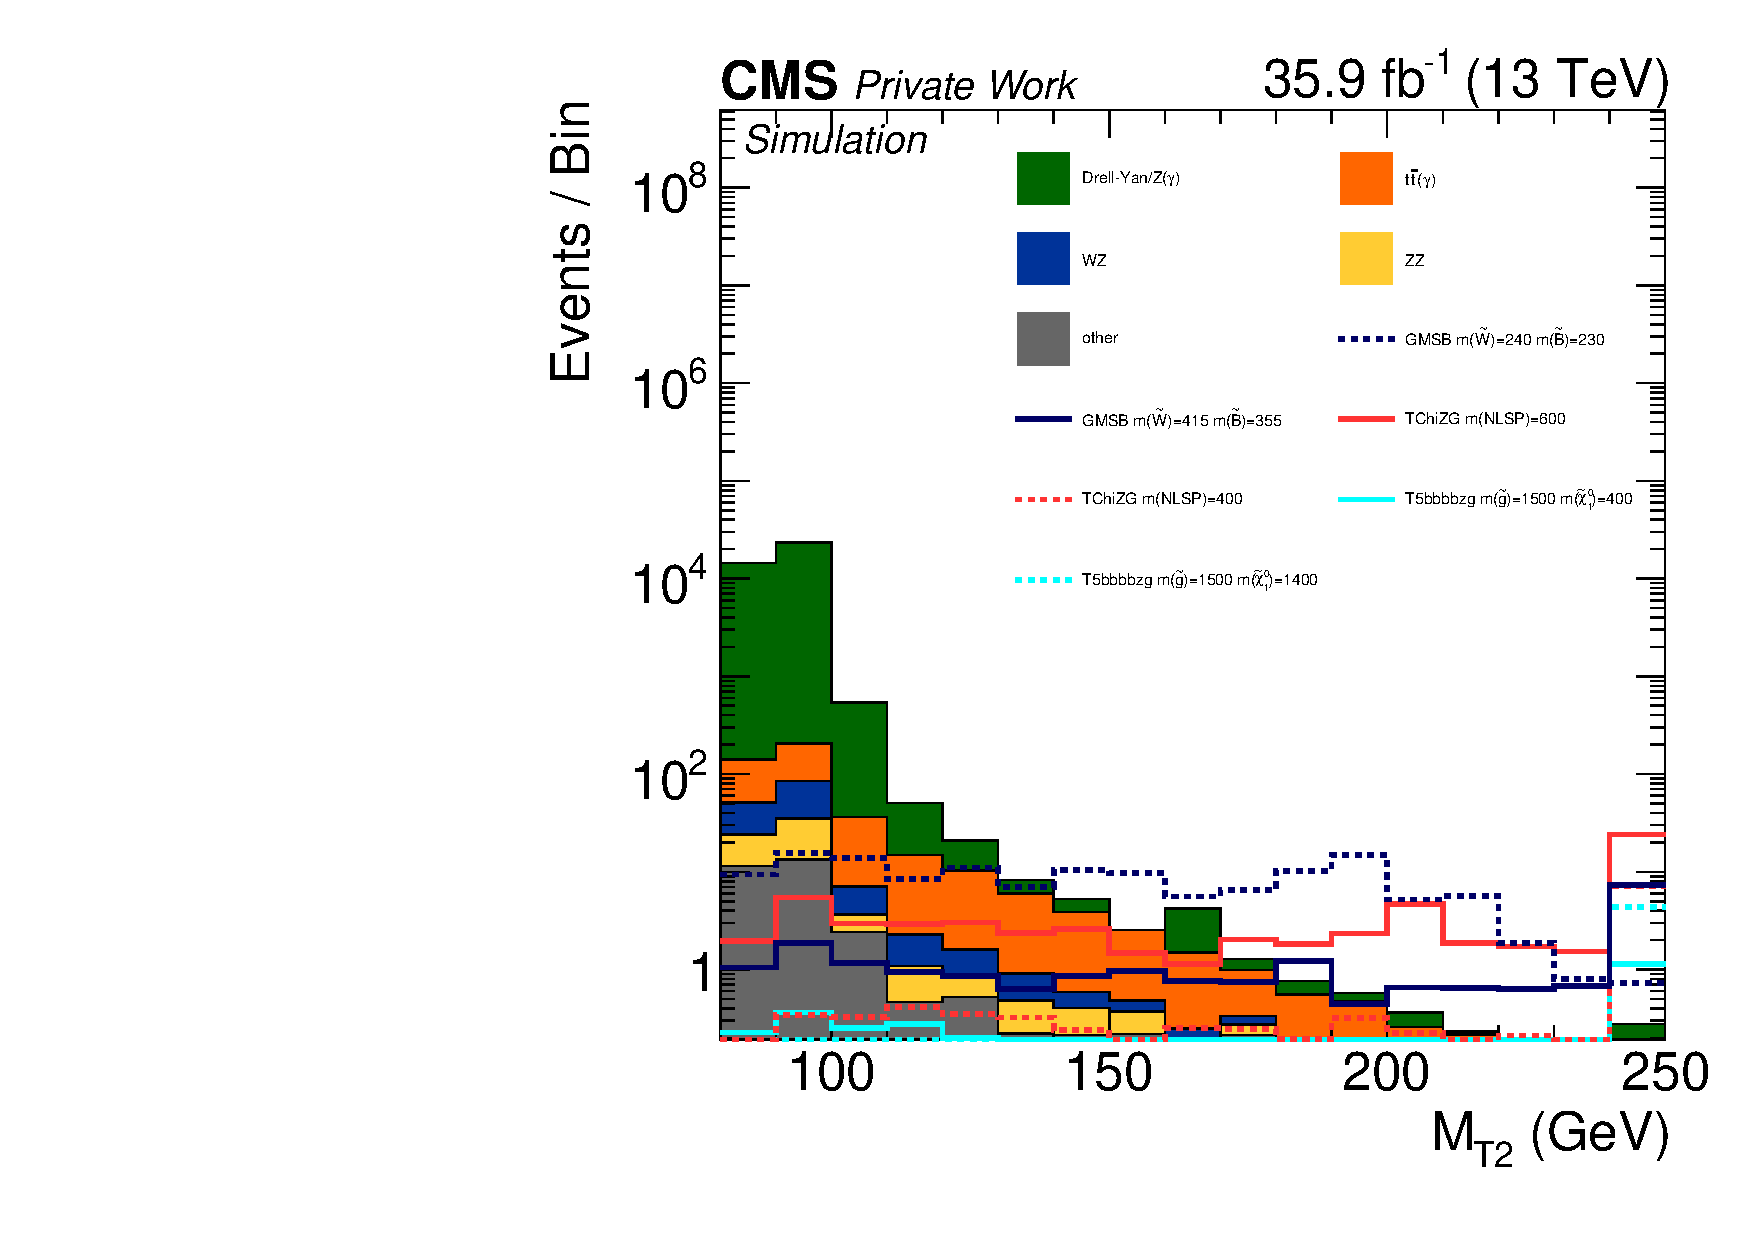
\includegraphics[width=\pairwidth]{figures/plots/onZ_LL_mt2_log}
 \caption{Stacked background events and events for different signal points against $\ptmiss$ (left) and $\mtTwo$ (right). Both are obtained from simulation. For each signal model two different signal points are shown. For their mass parameters refer to the legend in the plots.}
 \label{fig:SRvariables}
\end{figure}
The final SR is divided in two search bins in the $\ptmiss$ distribution, one ranging from $150$ to $200\GeV$, and the second one ranging from $200\GeV$ to infinity, see \refSec{sec:results}.

\subsection{Control regions}\label{sec:CR}
Different control regions (CRs) are defined for the four main background processes, in order to develop a background prediction for each background process. These CRs are built such that they are fully orthogonal to the signal region and among each other and include a large amount of events for precise studies and high purity. The main groups of backgrounds are $\ttbar(\PGg)$, DY/$\PZ(\PGg)$, $\PW\PZ$, and $\PZ\PZ$ production.

\subsubsection*{$\ttbar(\PGg)$ - control region}
To obtain a CR for the $\ttbar(\PGg)$ background, the flavor symmetry of the process is exploited. The two W bosons of the top quark decays can decay independently with the same probability to an electron or a muon, resulting in a similar number of same-flavor and different-flavor final state events. The different-flavor triggers are needed to guarantee a basis data set containing a sufficient number of events. In addition, the background can be studied in the same high $\ptmiss$ and $\mtTwo$ regions as the SR. The preselection criteria need to be adjusted accordingly, resulting in a CR definition of
\begin{itemize}
 \item exactly one different-flavor opposite-charge (DFOC) lepton pair ($\Pe\Pgm$),
 \item at least one photon,
 \item $\Delta R(\ell_1,\PGg)>0.3$ and $\Delta R(\ell_2,\PGg)>0.3$.
\end{itemize}
The invariant dilepton mass window requirement is removed from the preselection, since the reconstructed dilepton mass is not in coincidence with the Z boson mass. In contrast, it shows a broad distribution because the leptons are not originating from the same mother particle. The requirement being responsible for the orthogonality to the SR is the different dilepton flavor requirement.
\subsubsection*{Drell-Yan/$\PZ(\PGg)$ - control region}
The Drell-Yan/$\PZ(\PGg)$ background has nearly the same phenomenological topology as the SUSY signal, except for lower missing transverse momentum on average, since it mainly originates from mismeasurements of jets. The final control region definition additionally to the preselection is
\begin{itemize}
 \item $\ptmiss<100\GeV$.
\end{itemize}
This region is orthogonal to the SR due to the inverted $\ptmiss$ requirement.
\subsubsection*{$\PW\PZ$ - control region}
In order to obtain a high purity $\PW\PZ$ control region, the SFOC dilepton criteria are adjusted such that the fully leptonic decay of the diboson system is studied. As in the preselection, a SFOC lepton pair is required, but the additional lepton veto is inverted. Hence, the existence of a third lepton is required. Since the leptonic W boson decays are selected, with the help of additional $\ptmiss$ and $m_{T}$ requirements the purity of the selection of $\PW\PZ$ diboson production events is enhanced. The transverse mass $m_{T}$ is calculated using the third lepton and the missing transverse momentum, and is therefore an estimate for the $\PW$ boson mass. In the identification of the lepton pair belonging to the $\PZ$ boson, all combinations fulfilling flavor and charge requirements are tested. In case of multiple valid combinations, the combination with the invariant dilepton mass closest to the Z boson mass is chosen. To ensure a selection with a suitable amount of data, since the cross section for diboson production is rather low, the requirement of the existence of at least one photon from the preselection is removed. The final region selection is
\begin{itemize}
 \item exactly one SFOC lepton pair ($\Pe\Pe$ or $\PGm\PGm$),
 \item exactly one additional third lepton ($\Pe$ or $\Pgm$),
 \item $\Delta R(\ell_1,\PGg)>0.3$ and $\Delta R(\ell_2,\PGg)>0.3$,
 \item $81\GeV<m_{\ell\ell}<101\GeV$ (for the SFOC lepton pair),
 \item $\ptmiss>70\GeV$,
 \item $m_{T}(\ptvecmiss,\ptvec(\ell_3))>50\GeV$.
\end{itemize}
\subsubsection*{$\PZ\PZ$ - control region}\label{sec:VR}
The strategy to achieve a pure $\PZ\PZ$ diboson selection that does not overlap with the SR selection is very similar to the $\PW\PZ$ CR selection described above. By selecting events, where both $\PZ$ bosons decay leptonically to charged leptons ($\Pe\Pe$ or $\PGm\PGm$), per definition an exclusive control region is obtained. As in the $\PW\PZ$ CR selection, flavor and charge requirements are considered to construct $\Z$ boson candidates from the four selected leptons. In cases, where multiple valid solutions for the reconstruction of two $\PZ$ bosons exist, the possibility with the first Z boson candidate mass closest to the nominal Z boson mass is chosen. The second Z boson candidate has to fulfill a looser mass agreement compared to the first one. Also, the existence of a photon in the event is not required. In total, the selection criteria are
\begin{itemize}
 \item exactly two SFOC lepton pairs ($\Pe\Pe$ or $\PGm\PGm$),
 \item $\Delta R(\ell_1,\PGg)>0.3$ and $\Delta R(\ell_2,\PGg)>0.3$ for the first pair,
 \item $76\GeV<m_{\ell\ell}<106\GeV$ for the mass of the first Z boson candidate,
 \item $50\GeV<m_{\ell\ell}<130\GeV$ for the mass of the second Z boson candidate.
\end{itemize}
\subsubsection{Validation region}
An additional validation region (VR) is constructed, where the developed background predictions are verified by performing data-to-background prediction comparisons. Therefore, it is convenient to choose a VR close in phase space to the SR. This is achieved by applying the same selection requirements as for the SR, but demanding either the $\ptmiss$ or the $\mtTwo$ requirement to be inverted. The VR must also not overlap with the DY/$\PZ(\PGg)$ CR, thus a minimal $\ptmiss$ requirement needs to be imposed. The selection requirements for the VR in addition to the preselection are the following:
\begin{itemize}
 \item $\ptmiss>100\GeV$,
 \item either $\ptmiss<150\GeV$ or $\mtTwo>100\GeV$.
\end{itemize}
A visualization of the signal, validation, and DY/$\PZ(\PGg)$ control region definitions in the $\mtTwo$ - $\ptmiss$ plane can be found in \refFig{fig:Regions}. Two dimensional histograms for the number of expected events motivating the region definitions are shown in \refFig{fig:Regions2} for all background processes, together with distributions of different benchmark signal points for all three considered signal models.
\begin{figure}[tbp]
 \centering
 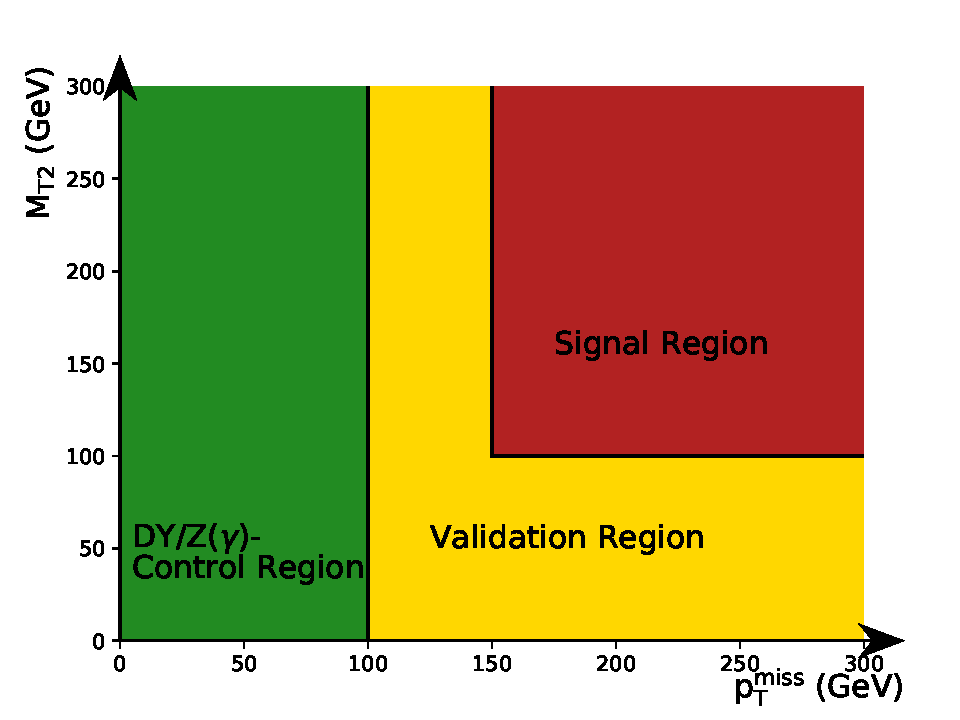
\includegraphics[width=\pairwidth]{figures/figures/regions}
 \caption{Visualization of the definition of the signal, validation, and DY/$\PZ(\PGg)$ control region in the $\mtTwo$ - $\ptmiss$ plane.}
 \label{fig:Regions}
\end{figure}
These distributions show also specific features of the considered signal models regarding important kinematic observables. Because the \texttt{TChiZG} model is a one parameter scan, and the only free parameter is the NLSP mass, together with the momentum of the NLSP it directly determines the maximum amount of transverse momentum for the decay products and thus directly the Z boson $\pt$ and the $\ptmiss$ originating from the gravitinos. Also, the endpoint of the $\mtTwo$ distribution is of the same order and coincide with the NLSP mass. Hence, $\ptmiss$ and $\mtTwo$ calculated from the bosons and $\ptmiss$ are strongly correlated.\\
In case of the strong SMS, it is not directly the case. Since this is a two dimensional parameter scan, the event kinematics also depend on the mass difference of the gluino and the NLSP mass, as discussed in \refSec{sec:SMS}. In cases where the mass difference is small, the kinematics evolve similar as for the EWK SMS, while for larger mass differences, as shown in \refFig{fig:Regions2}, the correlation between $\mtTwo$ and $\ptmiss$ is much weaker and the distributions are much broader. The distributions of the GMSB model behave similar to the electroweak SMS, depending on the wino and bino masses.\\
The signal events mainly populate the SR for all models, with small contributions in the CRs and the VR, while the majority of the background events contribute to the DY/$\PZ(\PGg)$ CR and a minor part to the VR. Only a minority of the background events are expected in the SR. Hence, in total a good separation between background and signal is achieved.

\begin{figure}[tbp]
 \centering
 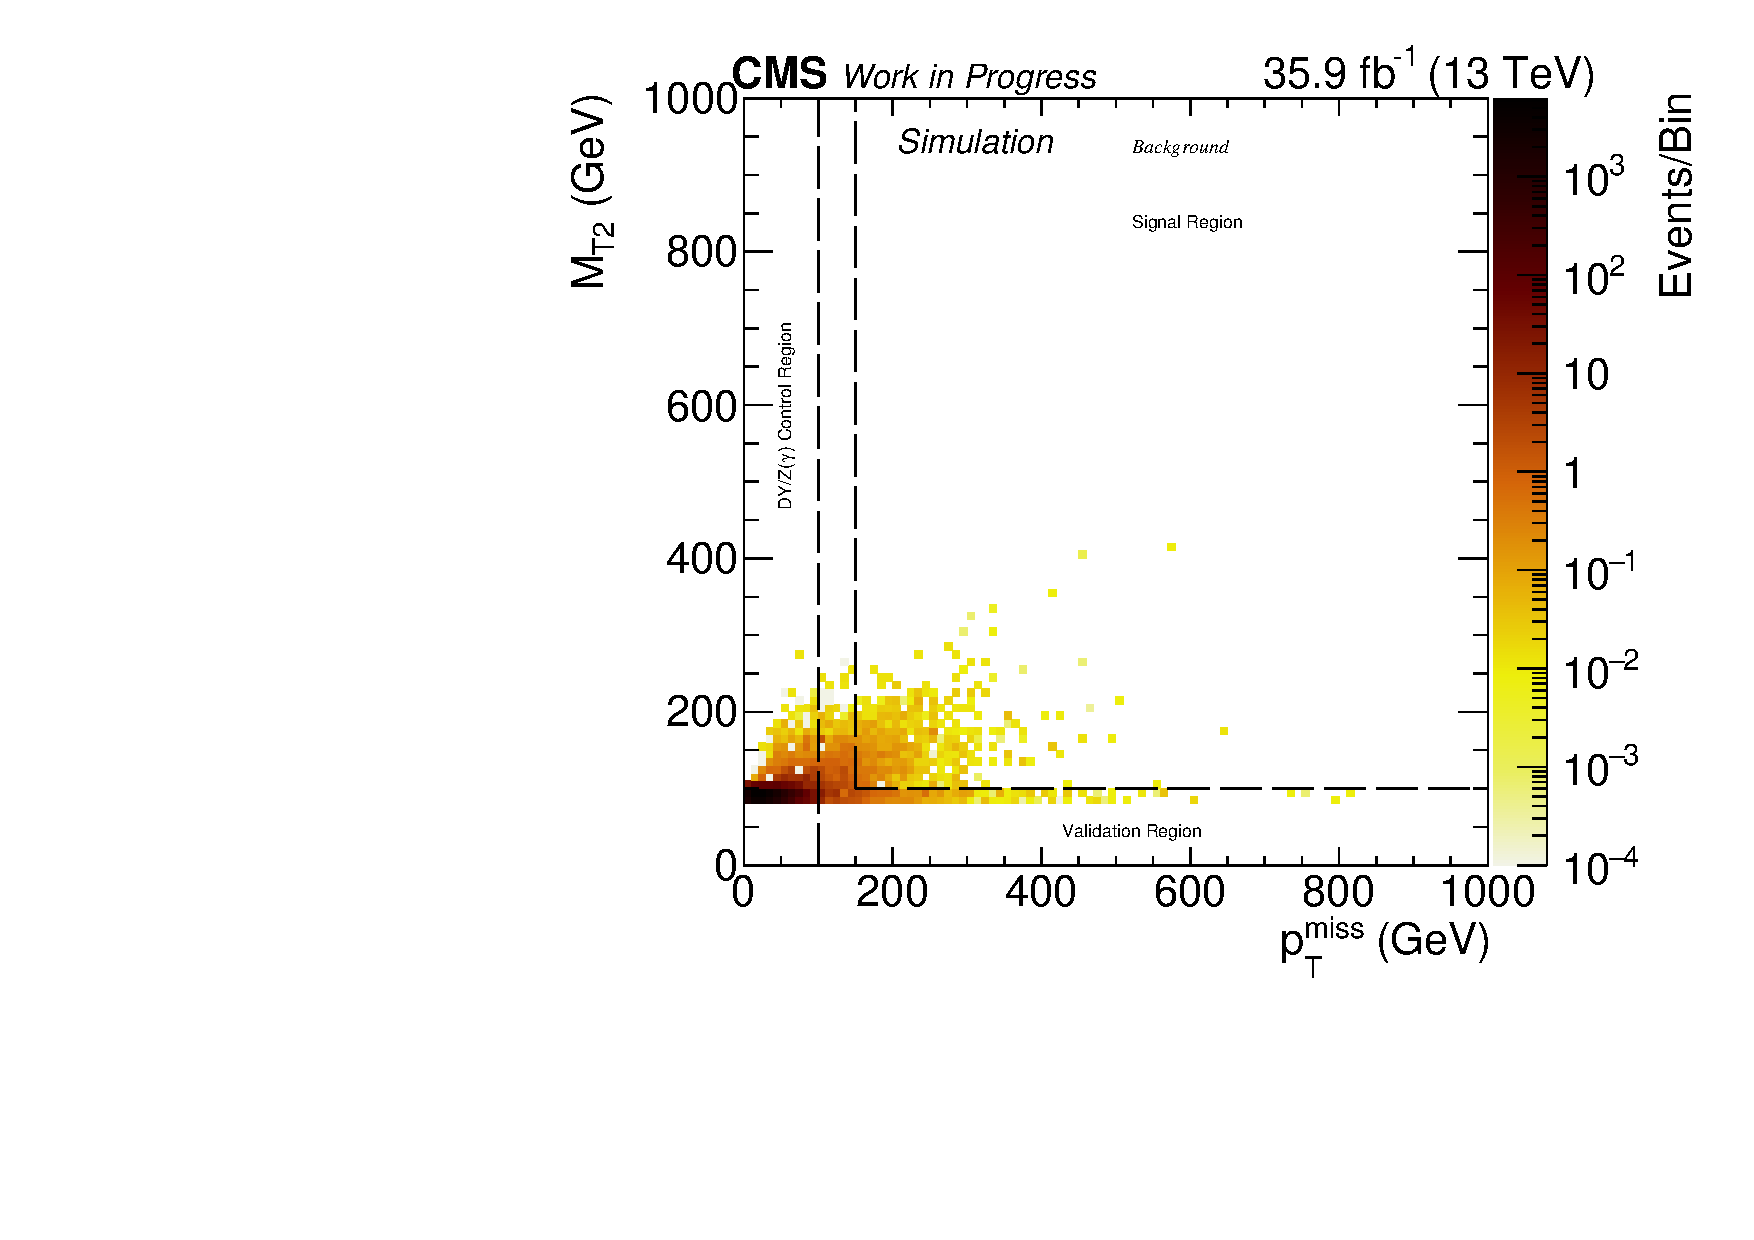
\includegraphics[width=\pairwidth]{figures/plots_2d/DataMC_sameHistograms_LL+signal_onZ__LL__MetMt2_bkg_}
 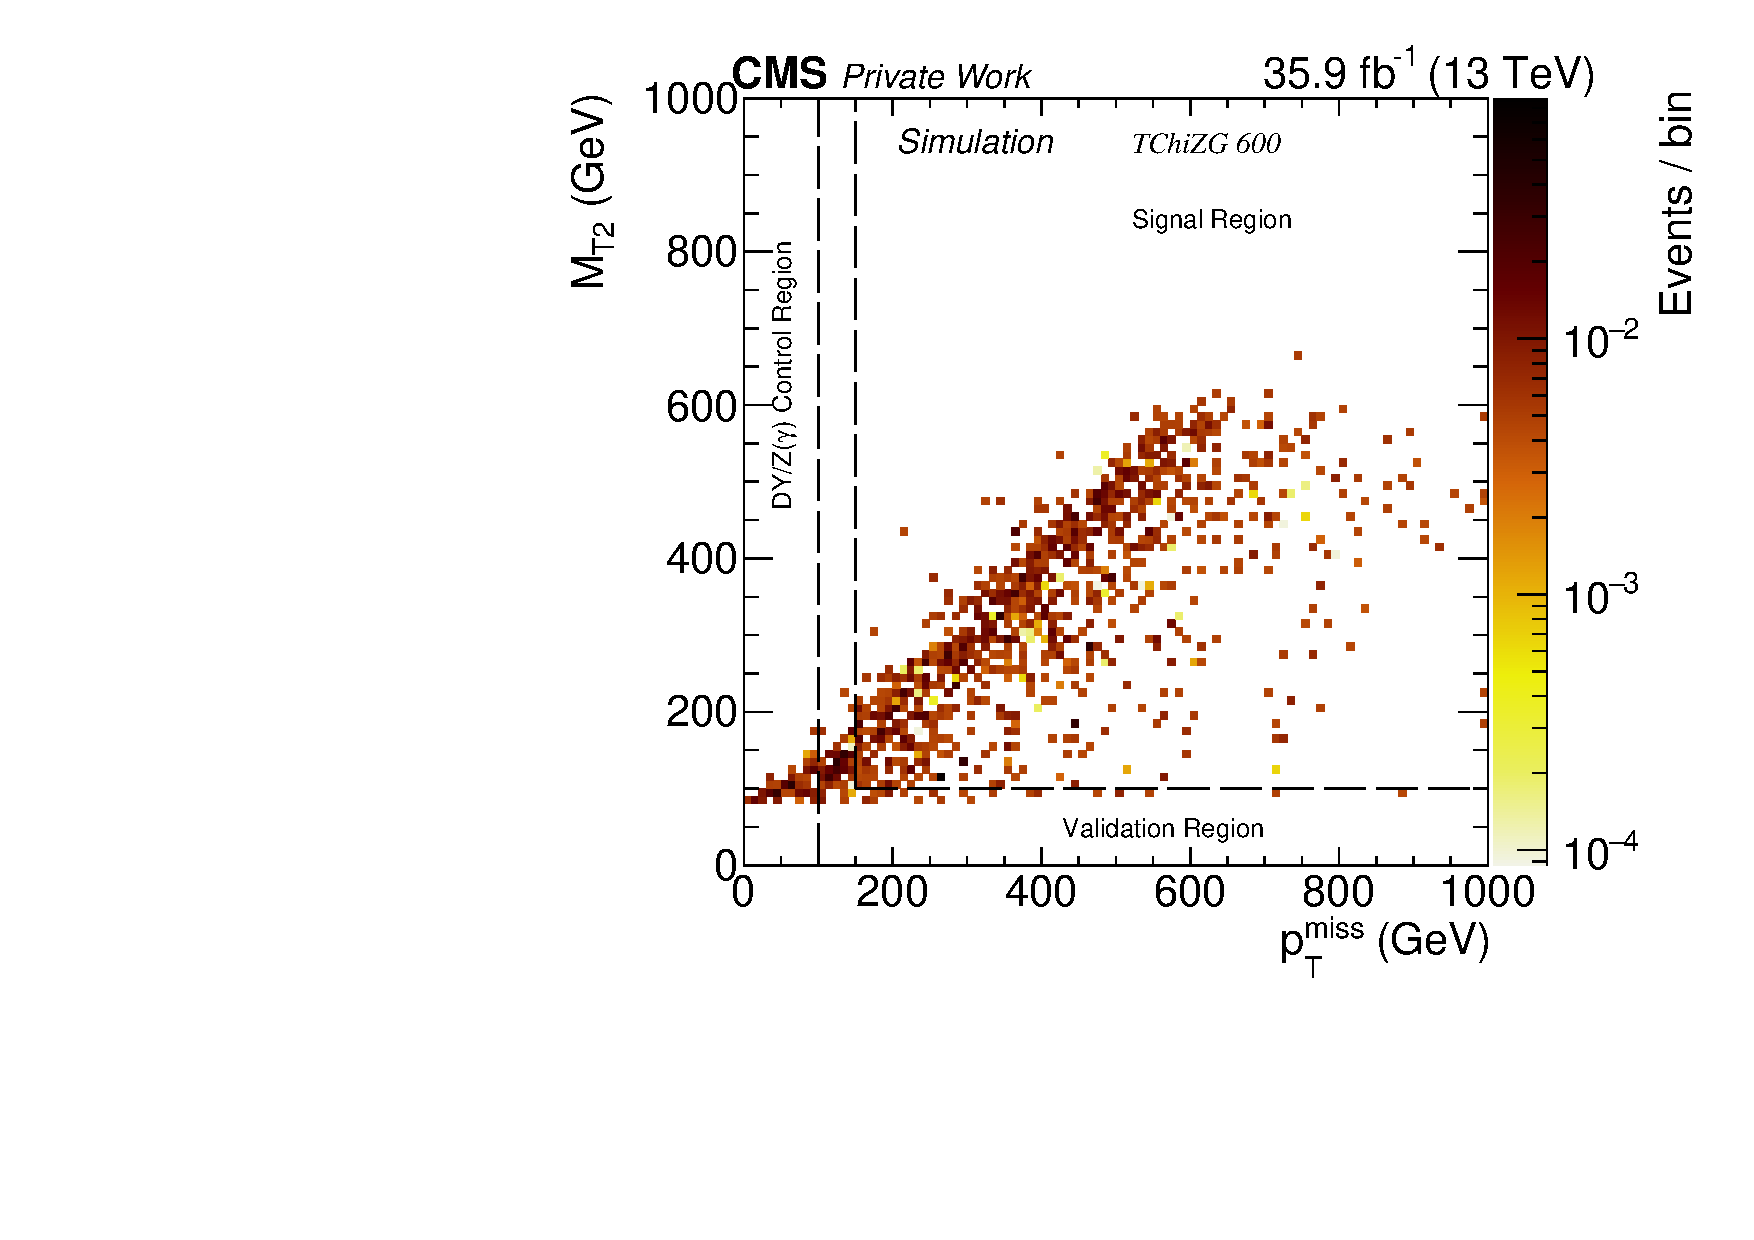
\includegraphics[width=\pairwidth]{figures/plots_2d/DataMC_sameHistograms_LL+signal_onZ__LL__MetMt2_SIG_tching600_}\\
 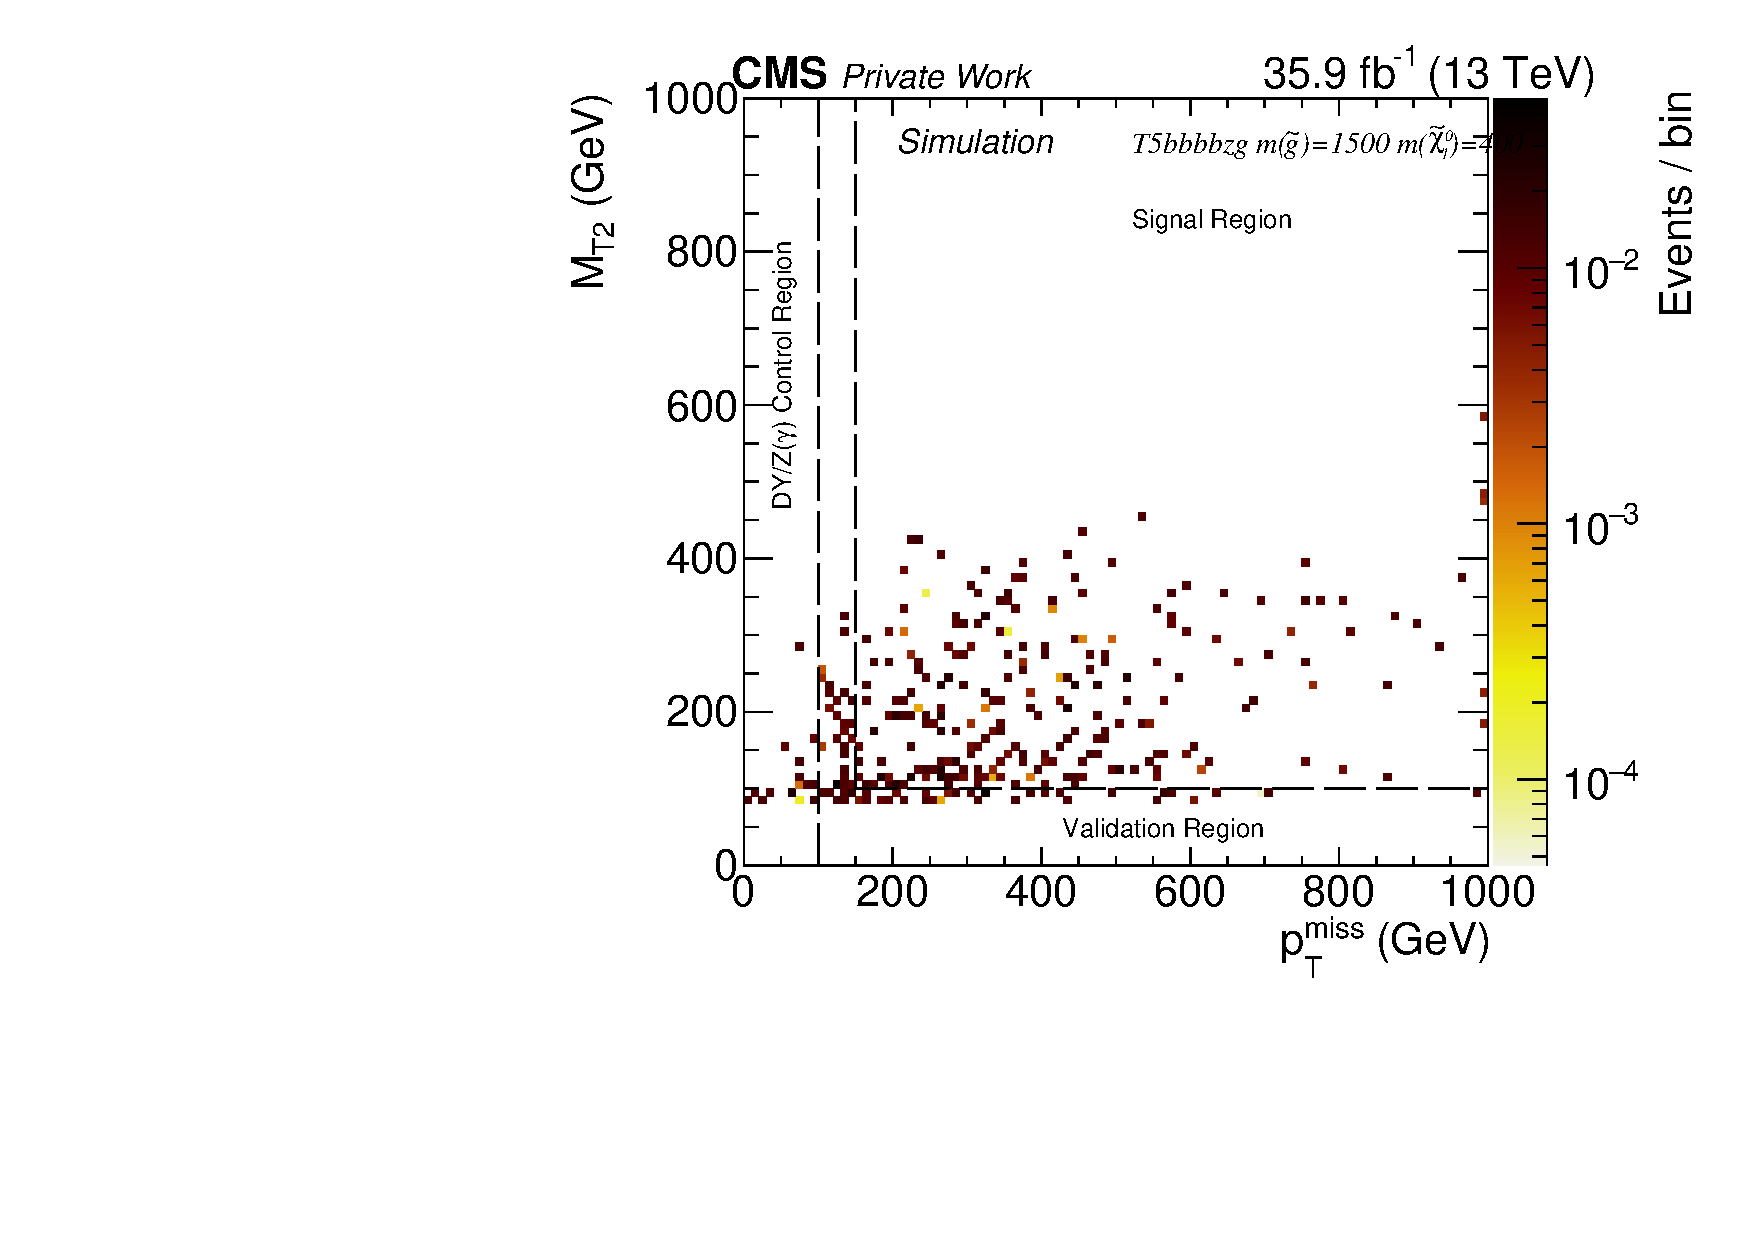
\includegraphics[width=\pairwidth]{figures/plots_2d/DataMC_sameHistograms_LL+signal_onZ__LL__MetMt2_SIG_t5bbbbzg_1500_400_}
 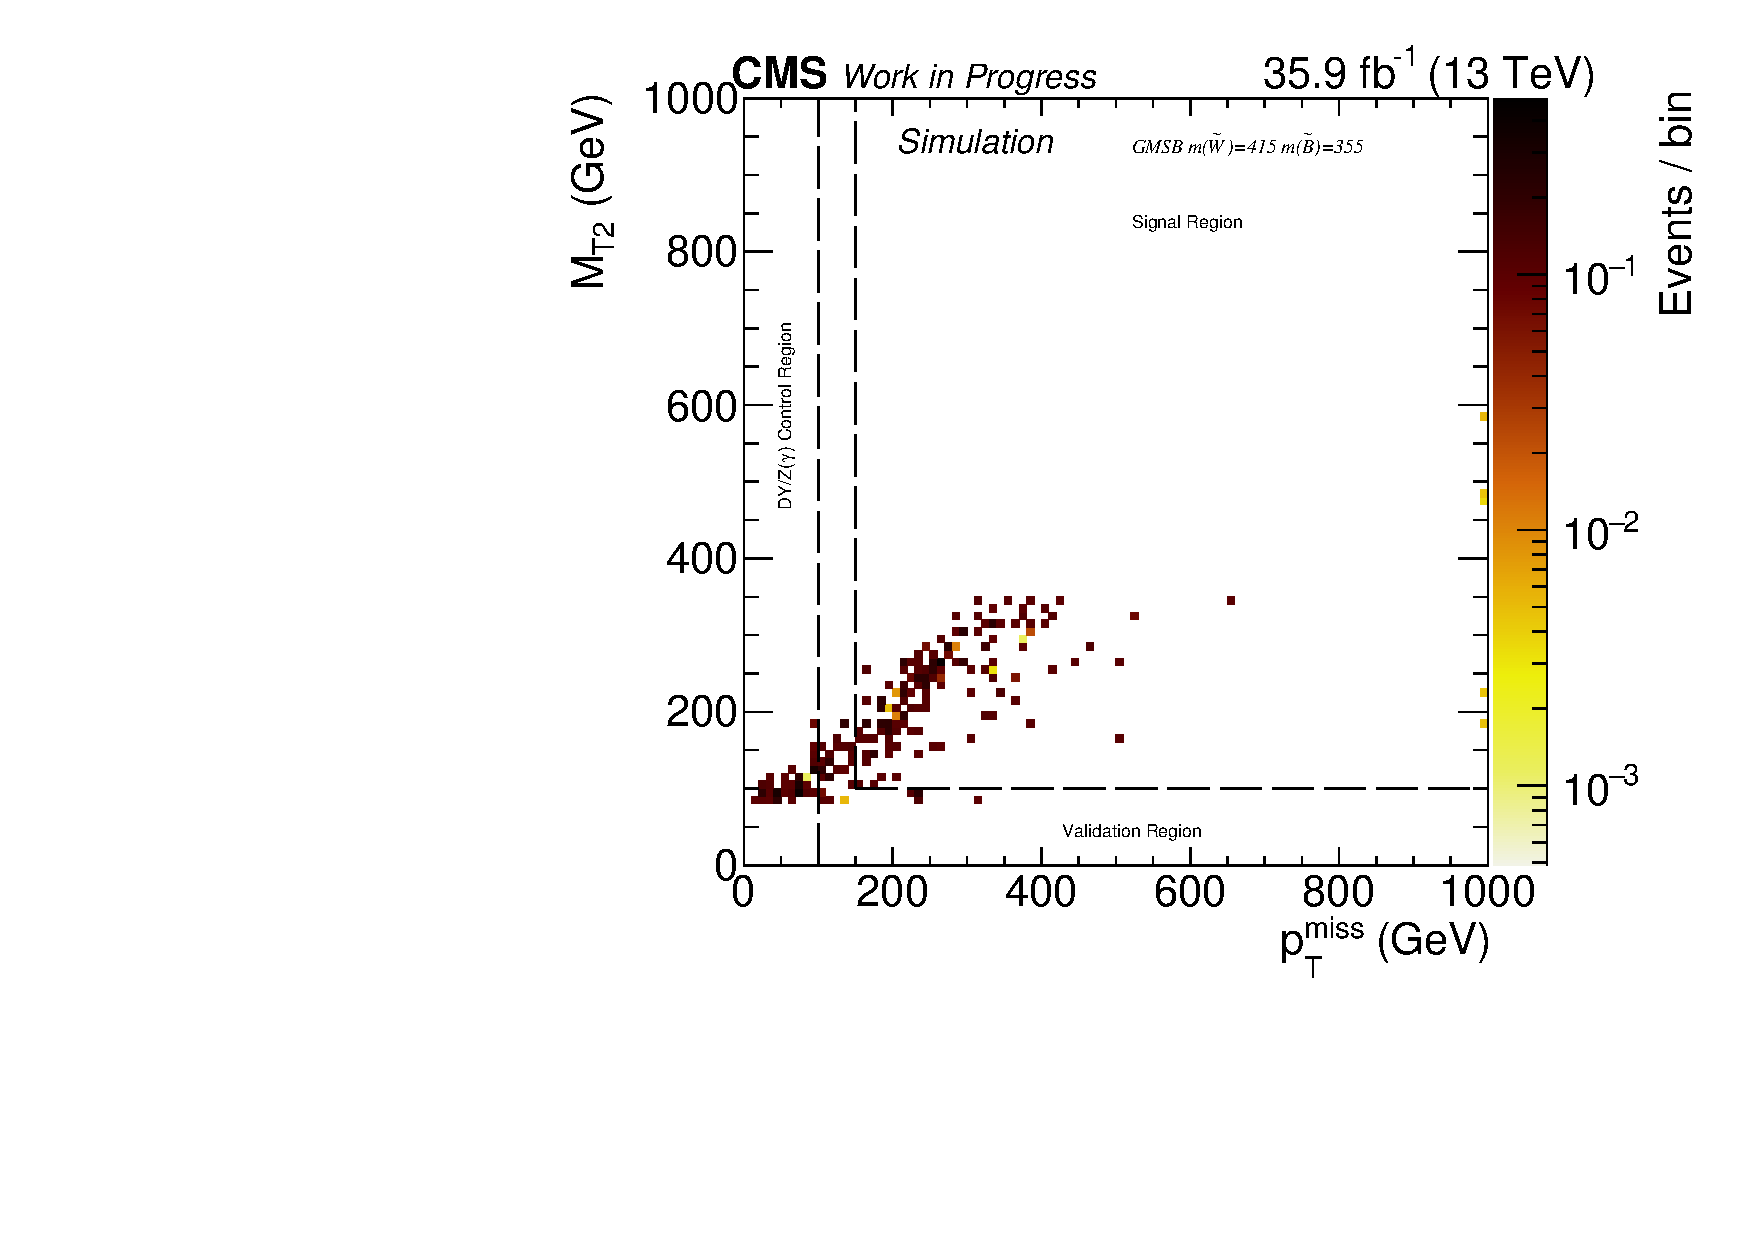
\includegraphics[width=\pairwidth]{figures/plots_2d/DataMC_sameHistograms_LL+signal_onZ__LL__MetMt2_SIG_gmsb_415_355_}
 \caption{Distribution of the total number of expected background events in the $\mtTwo$ - $\ptmiss$ plane (upper left). Distributions for the number of expected signal events for the \texttt{TChiZG} SMS with an NLSP mass of $600\GeV$ (upper right), the \texttt{T5bbbbZG} SMS with a gluino mass of $1.5\TeV$ and a neutralino mass of $400\GeV$ (bottom left), and the GMSB model with $m(\widetilde{W})=455\GeV$ and $m(\widetilde{B})=355\GeV$ (bottom right).}
 \label{fig:Regions2}
\end{figure}



\section{Background estimation}\label{sec:BKG}
In this section, the used background estimation methods are discussed, including the study of systematic effects. The total background is composed of $\ttbar(\PGg)$ production, Drell-Yan and $\PZ(\PGg)$ events, $\PW\PZ$ and $\PZ\PZ$ diboson production, and a remaining group of backgrounds ("other"), composed of, \eg, single top and triboson production (See \refSec{sec:Simulation} and \refSec{sec:CR}). The relative contributions for all background processes in the two SR bins are depicted in \refFig{fig:PieCharts}. The most dominant background is $\ttbar(\PGg)$, followed by $\PW\PZ$, $\PZ\PZ$, and Drell-Yan/$\PZ(\PGg)$.\\
The leptonic decays of the top pairs generated in association with a photon significantly contribute to the SR, because the final state signatures appear very similar to those of the SUSY models and the production cross section is very high. If both $\PW$ bosons decay leptonically, a SFOC lepton pair in connection with neutrinos can be produced, creating a large amount of $\ptmiss$ in the detector. Prompt photons can be produced in the hard interaction, or can be radiated off in the initial or the final state by participating charged particles. Since the two selected leptons of the $\ttbar$ system decay originate from different mother particles, the reconstructed invariant mass distribution shows is broad and shows no resonance. Due to the high cross section of the $\ttbar(\PGg)$ production, see \refTab{tab:MCsamples}, there is a sufficient probability to measure an invariant dilepton mass close to the Z boson mass although the two leptons do not emerge from it.\\
In the Drell-Yan process and in $\PZ\PGg$ production, an on-shell Z boson is produced, thus the $\m_{\ell\ell}$ requirement for the dileptons in the SR is fulfilled. Although a photon can be produced additionally, this background does not contribute significantly to the SR, because only nongenuine $\ptmiss$ is generated in the process due to mismeasurements and therefore the $\ptmiss$ distribution is steeply falling.\\
$\PW\PZ$ production is also an important background for this search, since the $\PW$ boson can decay leptonically and therefore creates a sufficient amount of genuine $\ptmiss$ to pass the SR requirements, but is also suppressed by the $\mtTwo$ requirement. While a photon can be generated in all possible radiation processes, an additional electron or jet originating from the $\PW$ boson can fake a photon signature in the detector. In cases of appearance of photons, events can contribute, where the additional lepton does not pass the acceptance, reconstruction, and identification criteria.\\
Lastly, the $\PZ\PZ$ event signature can be very similar to the one expected from the considered SUSY signals. One boson can decay to a pair of charged leptons, while the other decays to neutrinos leading to a large amount of $\ptmiss$ in the event. Together with FSR or ISR of a photon, $\PZ\PZ$ background events show a signature very similar to the signal topology.\\
If the different background processes are compared, the diboson processes have more similar event kinematics than the $\ttbar(\PGg)$ process compared to the signal processes, but due to the lower diboson production cross sections the $\ttbar(\PGg)$ background dominates the other contributions.
\begin{figure}[tbp]
 \centering
 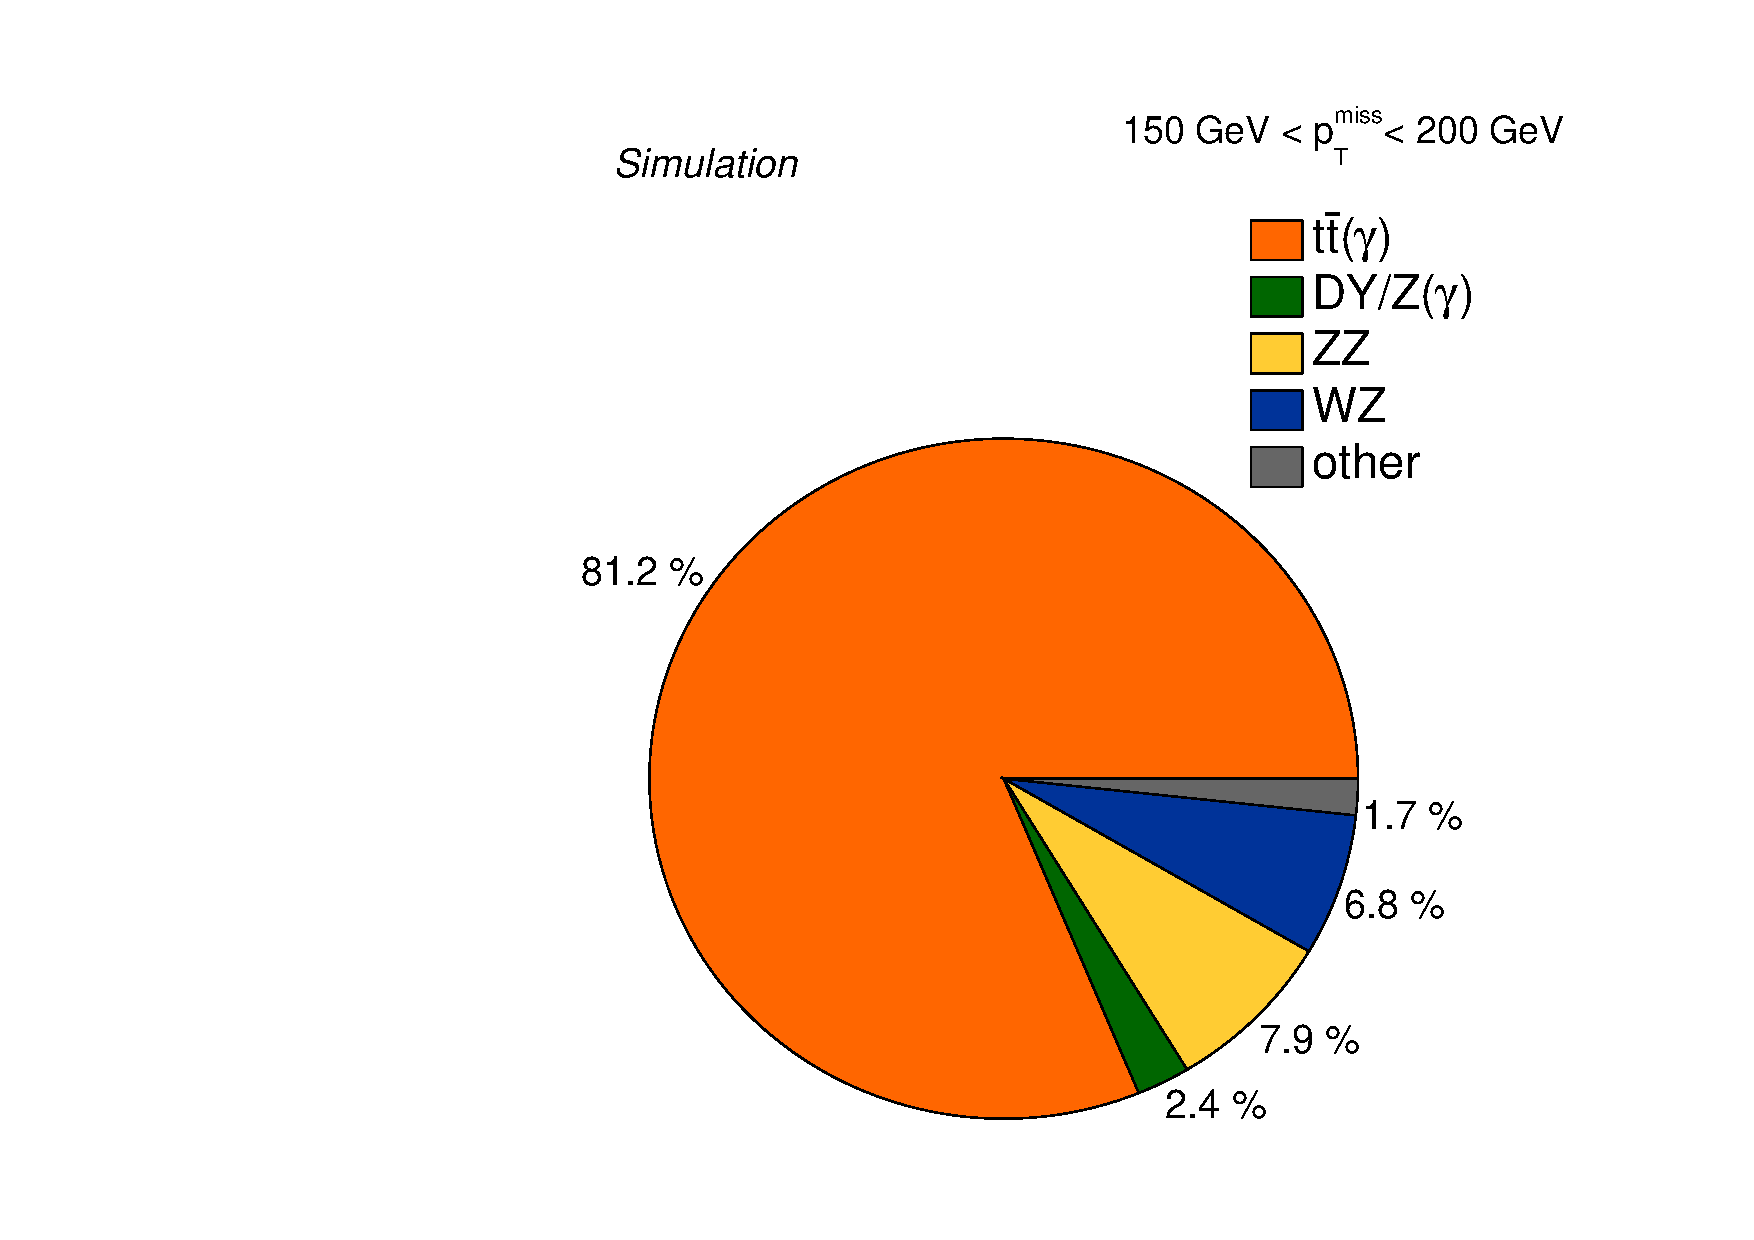
\includegraphics[width=\pairwidth]{figures/figures/pie1}
 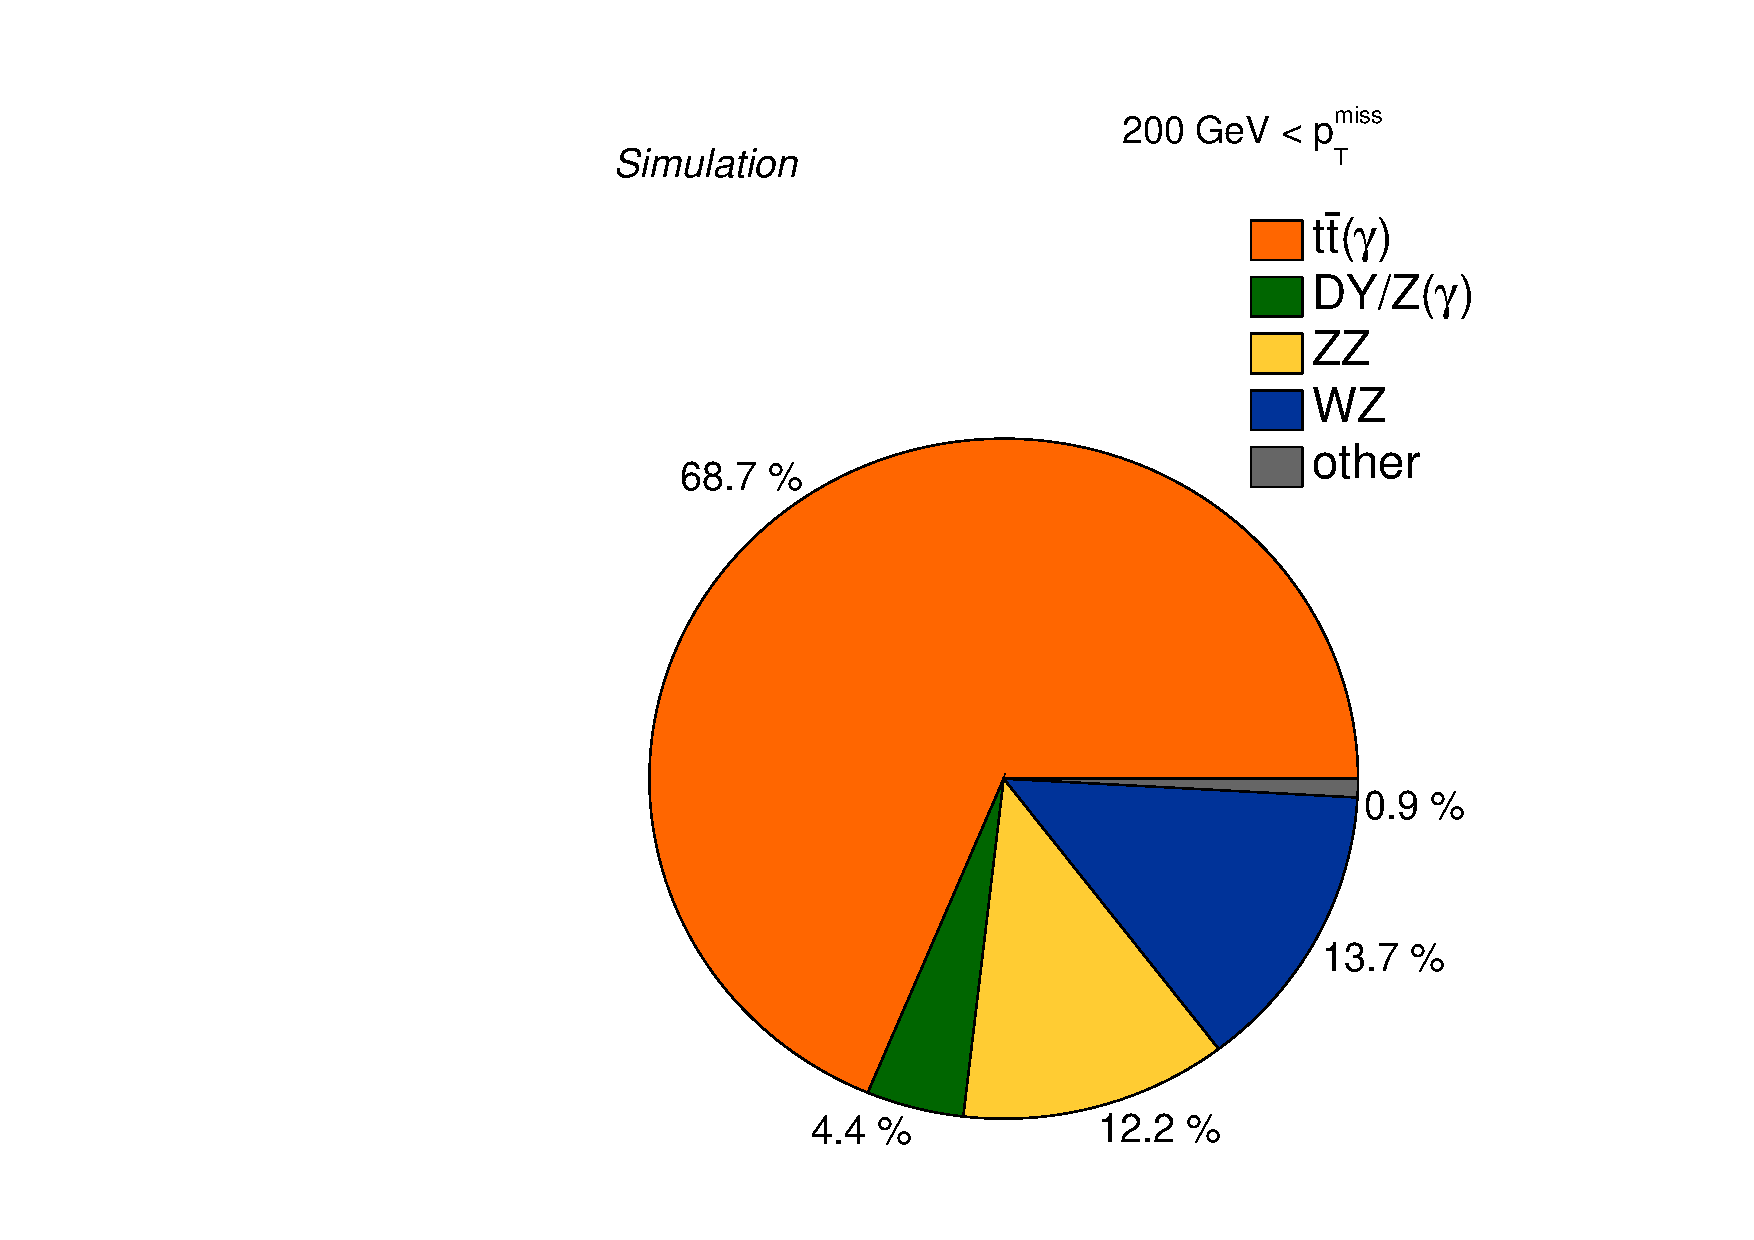
\includegraphics[width=\pairwidth]{figures/figures/pie2}
 \caption{Relative amounts for all groups of considered backgrounds for the two search bins in the SR.}
 \label{fig:PieCharts}
\end{figure}
The background prediction is based on simulation for all backgrounds. As mentioned in \refSec{sec:CR}, different CRs are developed, that are enriched with corresponding background events. In those CRs, scale factors (SF) $\alpha_i$ are calculated by scaling the simulation to the measured data yield. Contributions of other backgrounds in the CR are considered in the calculation by fixing their contribution. The SFs are calculated via the following formula:
\begin{align}
 1                        & = \frac{D}{F+\alpha_i\cdot B} \\
 \Longrightarrow \alpha_i & = \frac{D-F}{B},              
\end{align}
where $B$ is the number of background events that are to be scaled, $F$ the number of fixed background events, and $D$ the number of measured data events.
Due to the used method, which is performed similarly in each CR, possible uncertainties on the normalization of the predicted distributions cancel, and only uncertainties in the shape need to be considered, see~\refSec{sec:Syst}. The uncertainty arising from the SF calculation is purely of statistical origin, and is calculated via error propagation
\begin{equation}
 \sigma_{\alpha_i}^2 = \sigma_{D}^2 \cdot \left(\frac{D}{B}\right)^2 + \sigma_{F}^2 \cdot \left(\frac{F}{B}\right)^2 + \sigma_{B}^2 \cdot \left(\frac{D-F}{B^2}\right)^2,
\end{equation}
where $\sigma_i$ are the corresponding statistical uncertainties to $D$, $F$, and $B$. These are assumed to be uncorrelated Poissonian uncertainties, and can be calculated via $\sigma_i=\sqrt{N_i}$, where $N$ is the associated integral of events in the selection. In the case of simulation, for the calculation of the SF the normalized event yield is used, whereas in the error calculation the pure MC event count is considered to reflect the underlying statistical precision of the simulation. This method is referred to as the "integral method" in the following.\\
In each CR, all other background contributions have an influence, since their contributions are not negligible. Therefore, the order of SF determination can introduce a bias. To minimize this effect, the SFs are calculated in descending order of the purity of the background sample. At first, the $\PZ\PZ$ SF is determined, followed by DY/$\PZ(\PGg)$, $\ttbar(\PGg)$, and $\PW\PZ$. However, the background estimations are discussed in a different order, starting with the most important background, $\ttbar(\PGg)$. The systematic uncertainty arising from the choice of order is discussed in \refSec{sec:Syst}.\\
To strengthen the confidence in the outcome, Kolmogorov-Smirnov (KS)~\cite{KS} tests are performed to study the agreement of measured and predicted shape, which are based on the largest deviation between the two compared distributions. Resulting KS-values from the tests results are quoted on the corresponding plots for each individual distribution in the related sections. KS-values $\ll1$ indicate disagreement between the input distributions, otherwise the distributions are considered to match.\\\\
In order to study a possible bias of observables not well modeled within the simulation, additional cross checks are performed. Similar to the SF calculation in the integral method, SFs are determined via $\chi^2$-minimization in the same CRs. Albeit this method is somewhat correlated to the method explained above, it enables the possibility to study influences of different distributions in different binnings. Therefore, for the final SF determination the integral method is preferred over the $\chi^2$-method, since it is independent of the choice of any observable or binning and the resulting values for $\alpha_i$ agree between both methods. Thus, the $\chi^2$-fits serve only as additional cross-checks. In order to obtain the SF via $\chi^2$-minimization, the $\alpha_{i}$ is varied in a range in small steps for each binning and distribution, and for every iteration the simulation is scaled and the $\chi^2$ is calculated, which is defined as:
\begin{equation}
 \chi^2=\sum_i^{N_{bins}} \frac{\left(N_{i}^{obs}-N_{i}^{pred}\right)^2}{N_{i}^{pred}}.
\end{equation}
The best fit value is determined to be at the minimum of the $\chi^2$-distribution, which is obtained by fitting a polynomial of fourth grade to the $\chi^2$-distribution. Ideally the measured $\chi^2$-distribution would be described by a parobola, but in order to account for asymmetries in the determined distribution, a higher order polynomial is chosen as the fit function. In addition, the fits do not have a statistical influence, but are only needed to extract the best fit value and its uncertainty, which is also of statistical origin. It is calculated by taking the difference between the best fit value and the values, corresponding to $\chi^2=\chi^2_{BestFit}+1$. An example fit in the $\ptmiss$ distribution is shown in \refSec{sec:ttbar} in the discussion of the $\ttbar(\PGg)$ background estimation. The number of degrees of freedom ($ndf$) is given by the number of bins used to obtain the $\chi^2$-distribution reduced by the number of parameters that are being optimized. The only free parameter is $\alpha_{i}$, so $ndf$ equals the number of bins subtracted by unity.\\
After determining all SFs, the background prediction is tested in the VR. Therefore, the simulated backgrounds in the VR are scaled accordingly, and the result is investigated, see \refSec{sec:Validation}.



\subsection{Top pair production}\label{sec:ttbar}
As shown in \refFig{fig:PieCharts}, the main background contribution is $\ttbar(\PGg)$, which is composed of standard top pair production with and without photon radiation, and top-pair production in association with a photon, while the latter dominates. Both compositions are determined together by rescaling the simulation, such that the integral of events of the simulation in the CR matches the integral of events in data as explained in \refSec{sec:BKG}. The overall purity of the selection is of the order of $85\%$.
% For the scaled event yields, only weights to account for the trigger efficiency correction and a global weight as mentioned in \refSec{sec:Simulation} to normalize the simulation to the physical expectation are made use of.
% \begin{table}[tbp]
%  \centering
%  \caption{Yields in the $\ttbar(\PGg)$ CR for the pure simulation and measured data.}
%  \label{tab:CRTT}
%  \begin{tabular}{llll}
%
%   process      & raw simulation & simulation & data                  \\\hline
%   $\ttbar$     & 12077          & 416.93     &                       \\
%   $\ttbar\PGg$ & 128396         & 1420.19    &                       \\\hline\hline
%   sum          & 140473         & 1837.12    & \multirow{2}{*}{1750} \\
%   other        & 14631          & 275.25     &
%  \end{tabular}
% \end{table}
With the integral method applied, the SF is obtained and given by
\begin{equation}\label{eq:AlphaTT}
 \alpha_{\ttbar(\PGg)}=0.80 \pm 0.03 (stat.) [\hat{=}4.0\%].
\end{equation}
After application of $\alpha_{\ttbar(\PGg)}$, the numbers of events in data and simulation match per definition.\\
Since the analyzed final state in this CR is very sensitive to higher order effects such as jet and photon radiation, and complex matrix elements are needed to describe the hard interaction, a SF differing from unity meets the expectation. NNLO electroweak effects can cause negative corrections for example due to destructive terms in higher order corrections.
The uncertainty of the order of $4\%$ indicates, that a sufficient number of events is present in the corresponding CR.\\
The resulting prediction shows a good agreement with data, as can be seen from the $\ptmiss$ and $\mtTwo$ distributions in the CR after rescaling in \refFig{fig:CRTT}. The uncertainty of the fit method is of statistical origin, and is treated as a systematic uncertainty in the following. The agreement of additional important observables, such as the transverse momentum of the photon and both leptons, is also investigated, and no systematic deviation was found.
\begin{figure}[tbp]
 \centering
 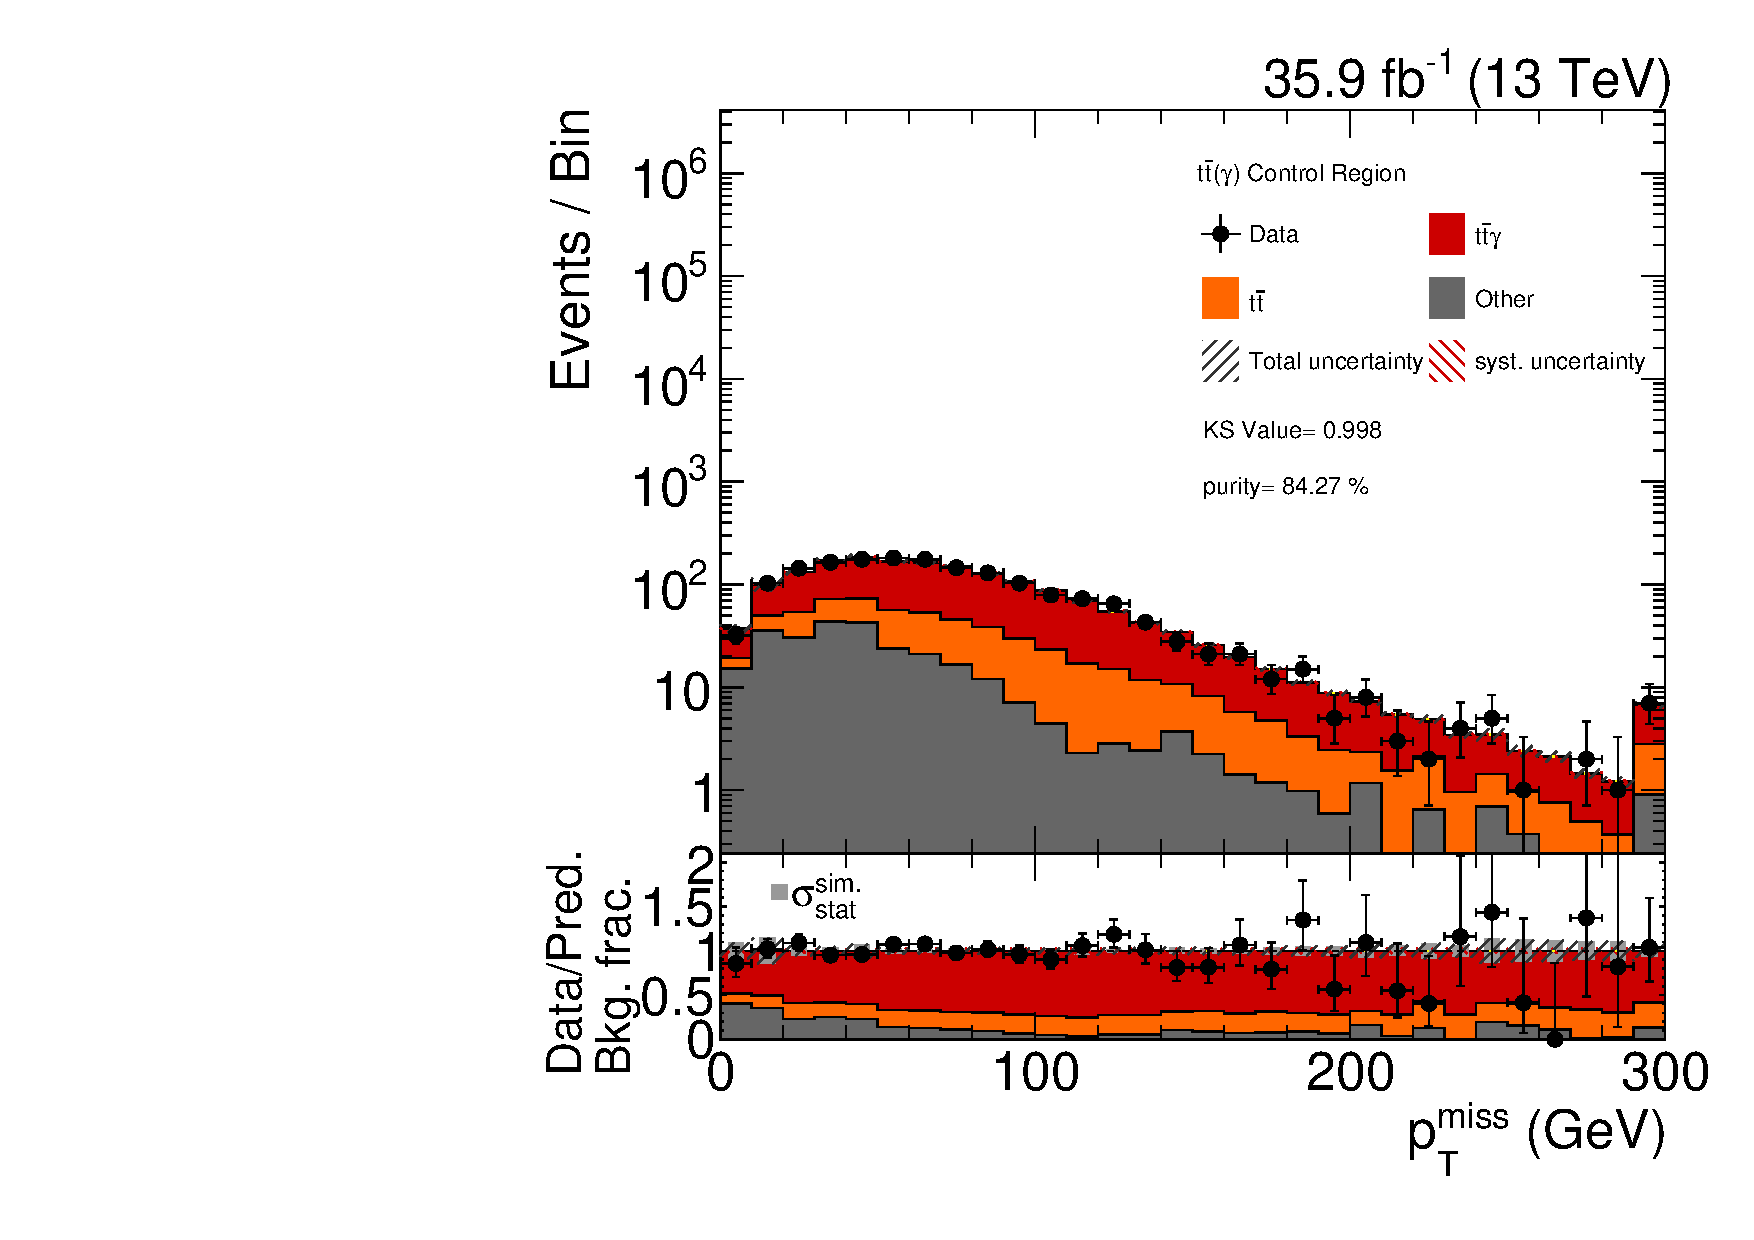
\includegraphics[width=\pairwidth]{figures/plots_CR_tt/CRTT_EM_nom_met_log}
 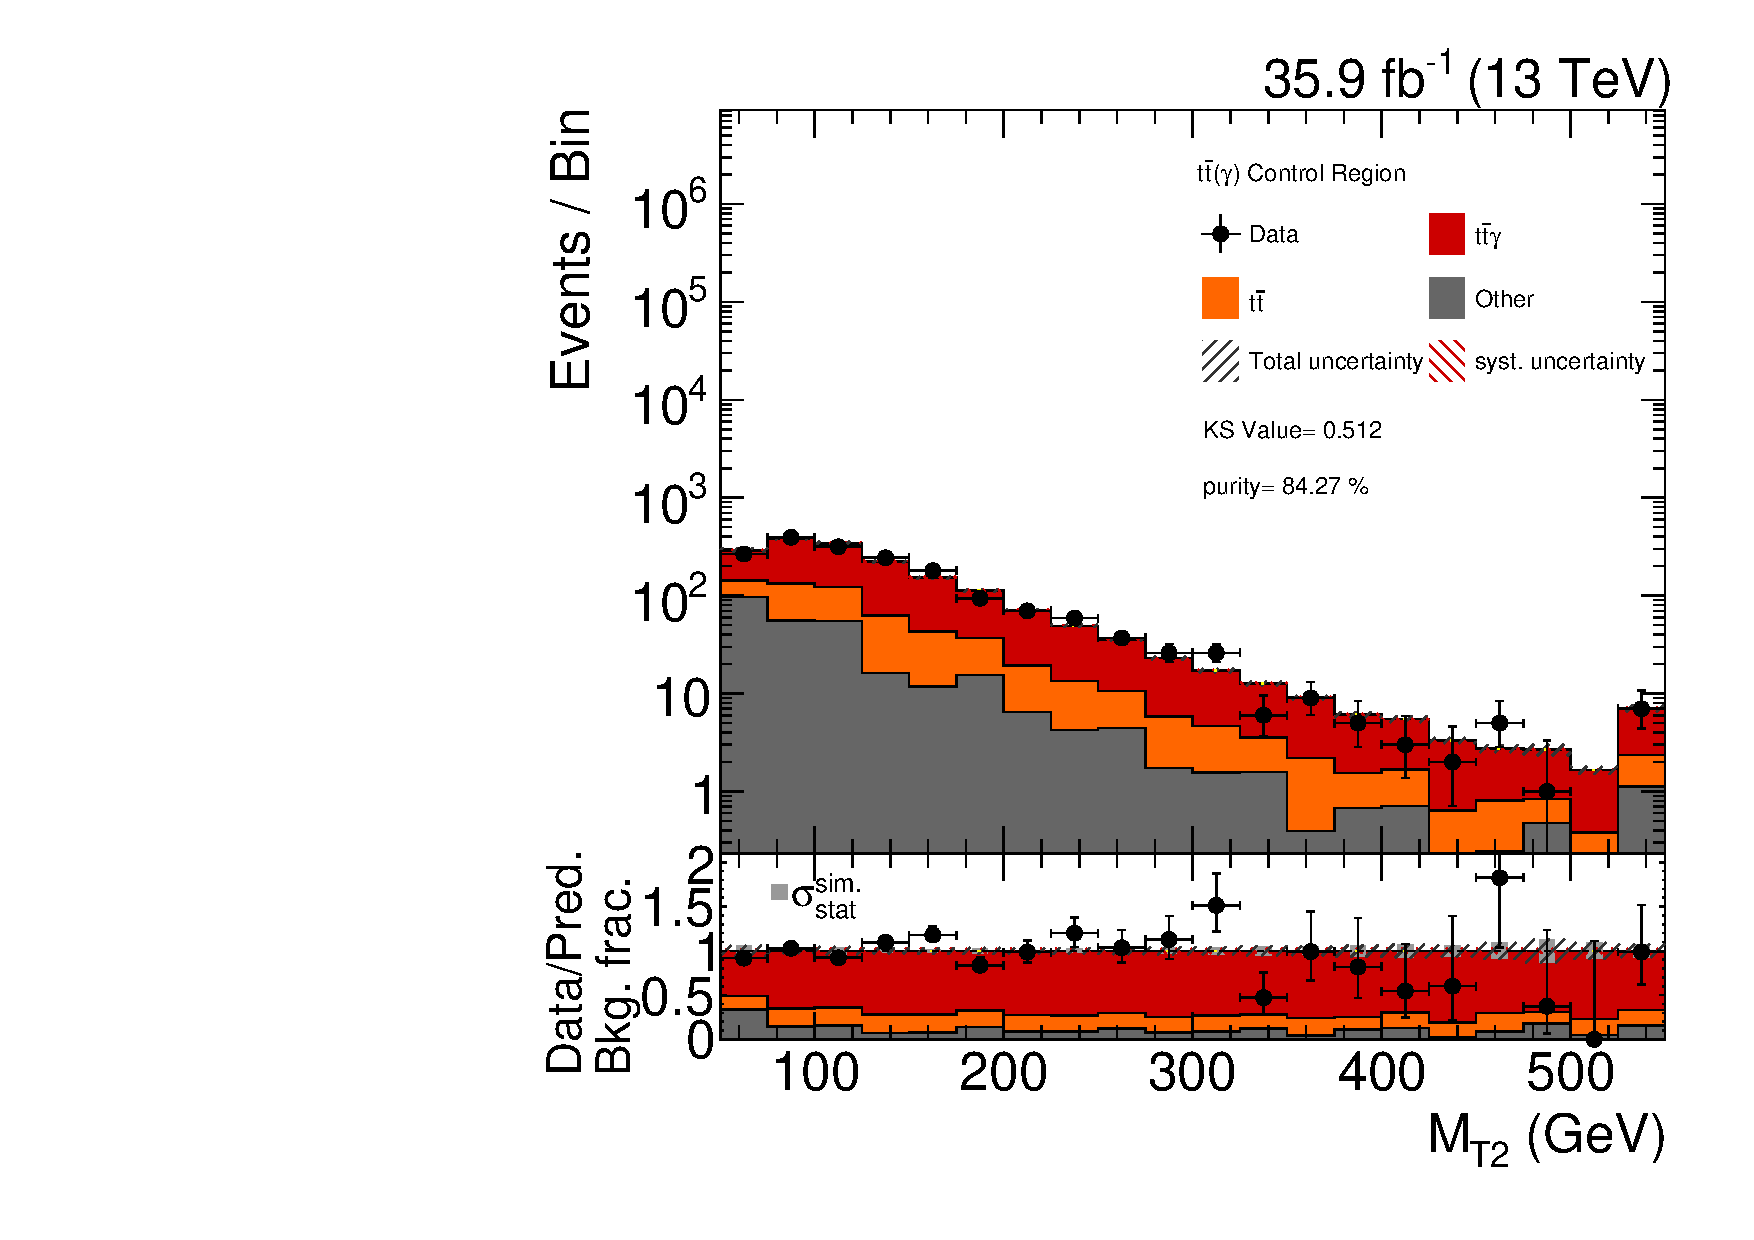
\includegraphics[width=\pairwidth]{figures/plots_CR_tt/CRTT_EM_nom_mt2_log}
 \caption{Comparisons between data and rescaled simulation in the $\ttbar(\PGg)$ CR in the $\ptmiss$ and $\mtTwo$ distribution. Below each plot, a ratio between data and prediction is shown. The uncertainty bands correspond to the systematic (red) and total uncertainty (gray). In addition, in the ratio plot the relative composition of the backgrounds is visualized. KS-values for the performed Kolmogorov-Smirnov test and the selection purity are also quoted.}
 \label{fig:CRTT}
\end{figure}
Additional statistical checks, such as Kolmogorov-Smirnov tests and $\chi^2$-fits, as explained above are also performed. The resulting KS-values of the Kolmogorov-Smirnov tests quoted in each plot indicate a good shape agreement.\\
The resulting curves of the $\chi^2$-fit distributions, see \refFig{fig:chiTT} left for an example fit in the $\ptmiss$ distribution, are smooth, indicating a proper performance of the fit. A comparison of all obtained SFs for the different setups and the SF obtained by the integral method is shown in \refFig{fig:chiTT} right. No significant deviation is observed, and all SFs are in agreement with each other. Hence, the scaling of the $\ttbar(\PGg)$ background seems stable and well described in the CR.
\begin{figure}[tbp]
 \centering
 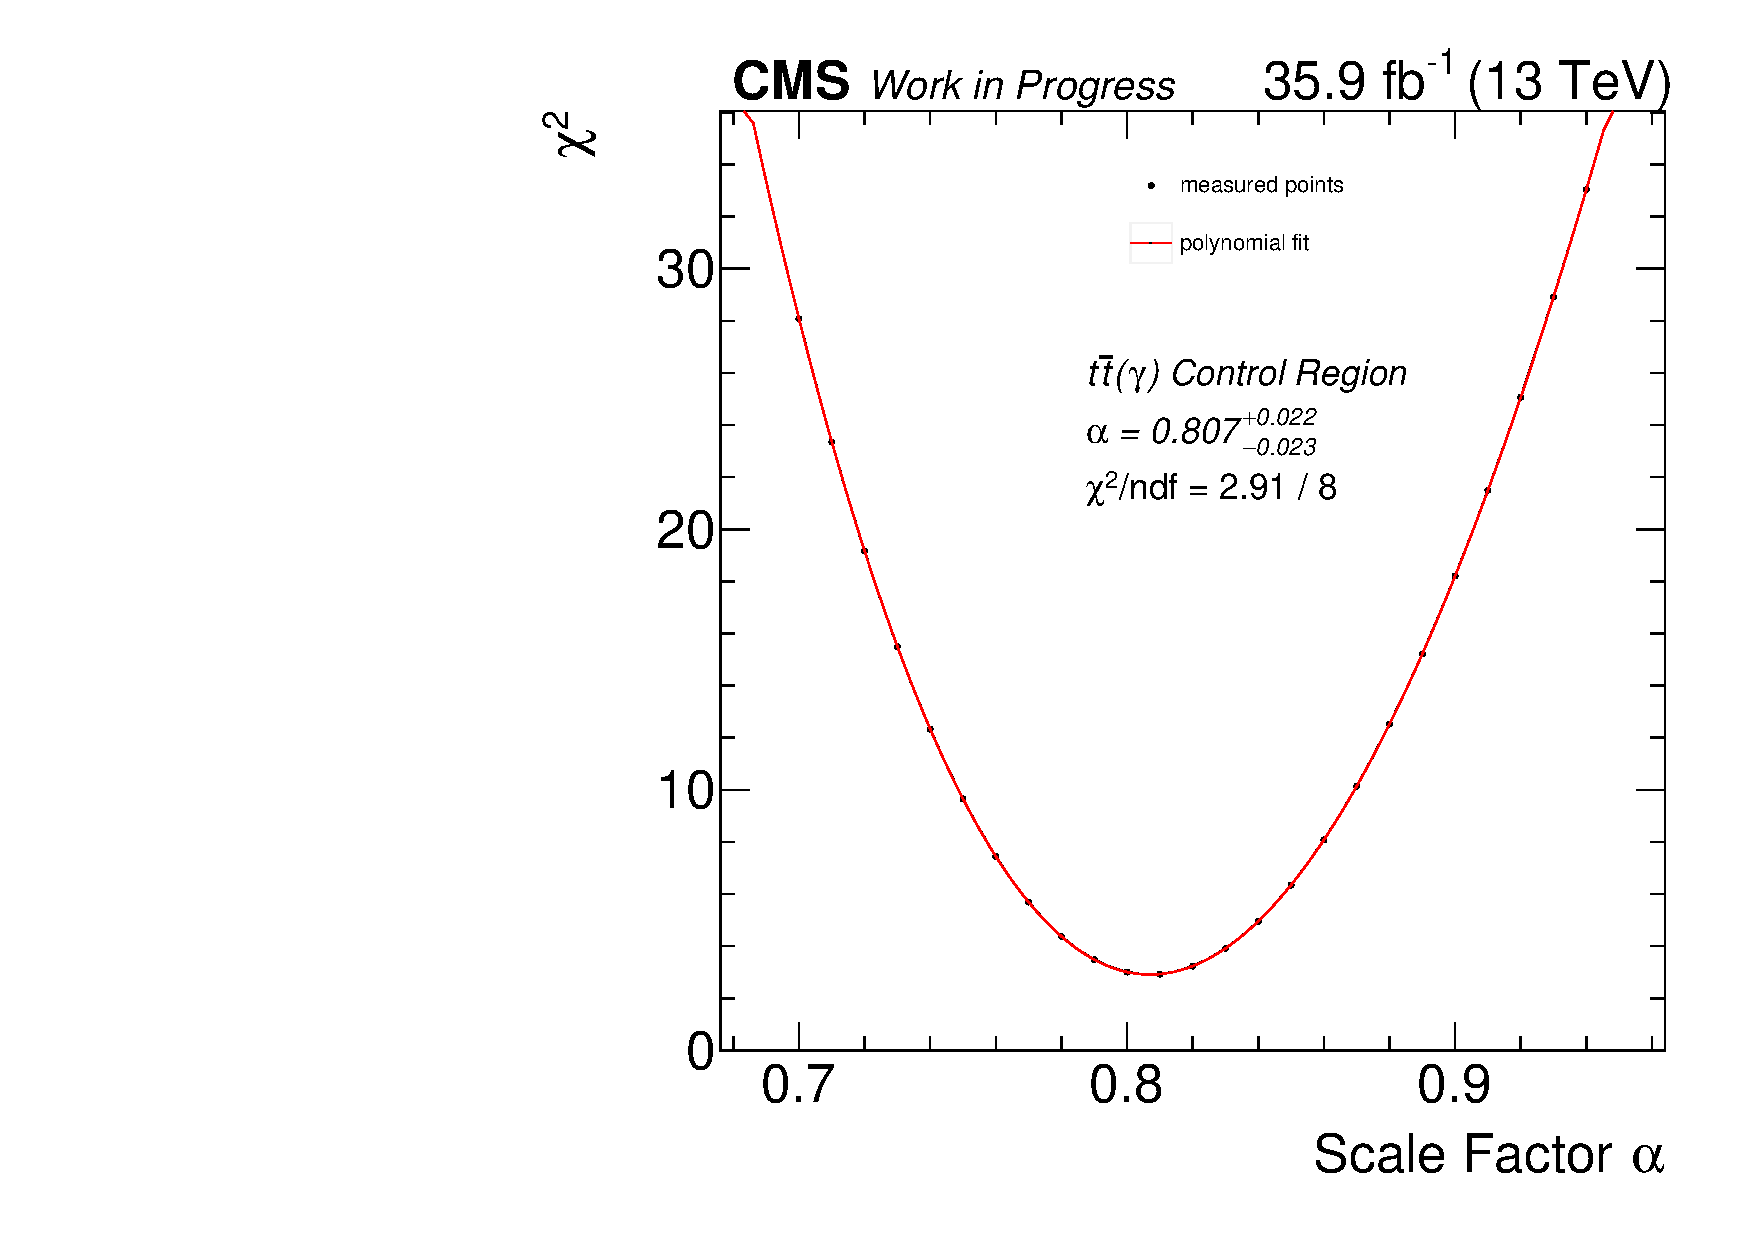
\includegraphics[width=\pairwidth]{figures/plots_CR/chi/TT_met}
 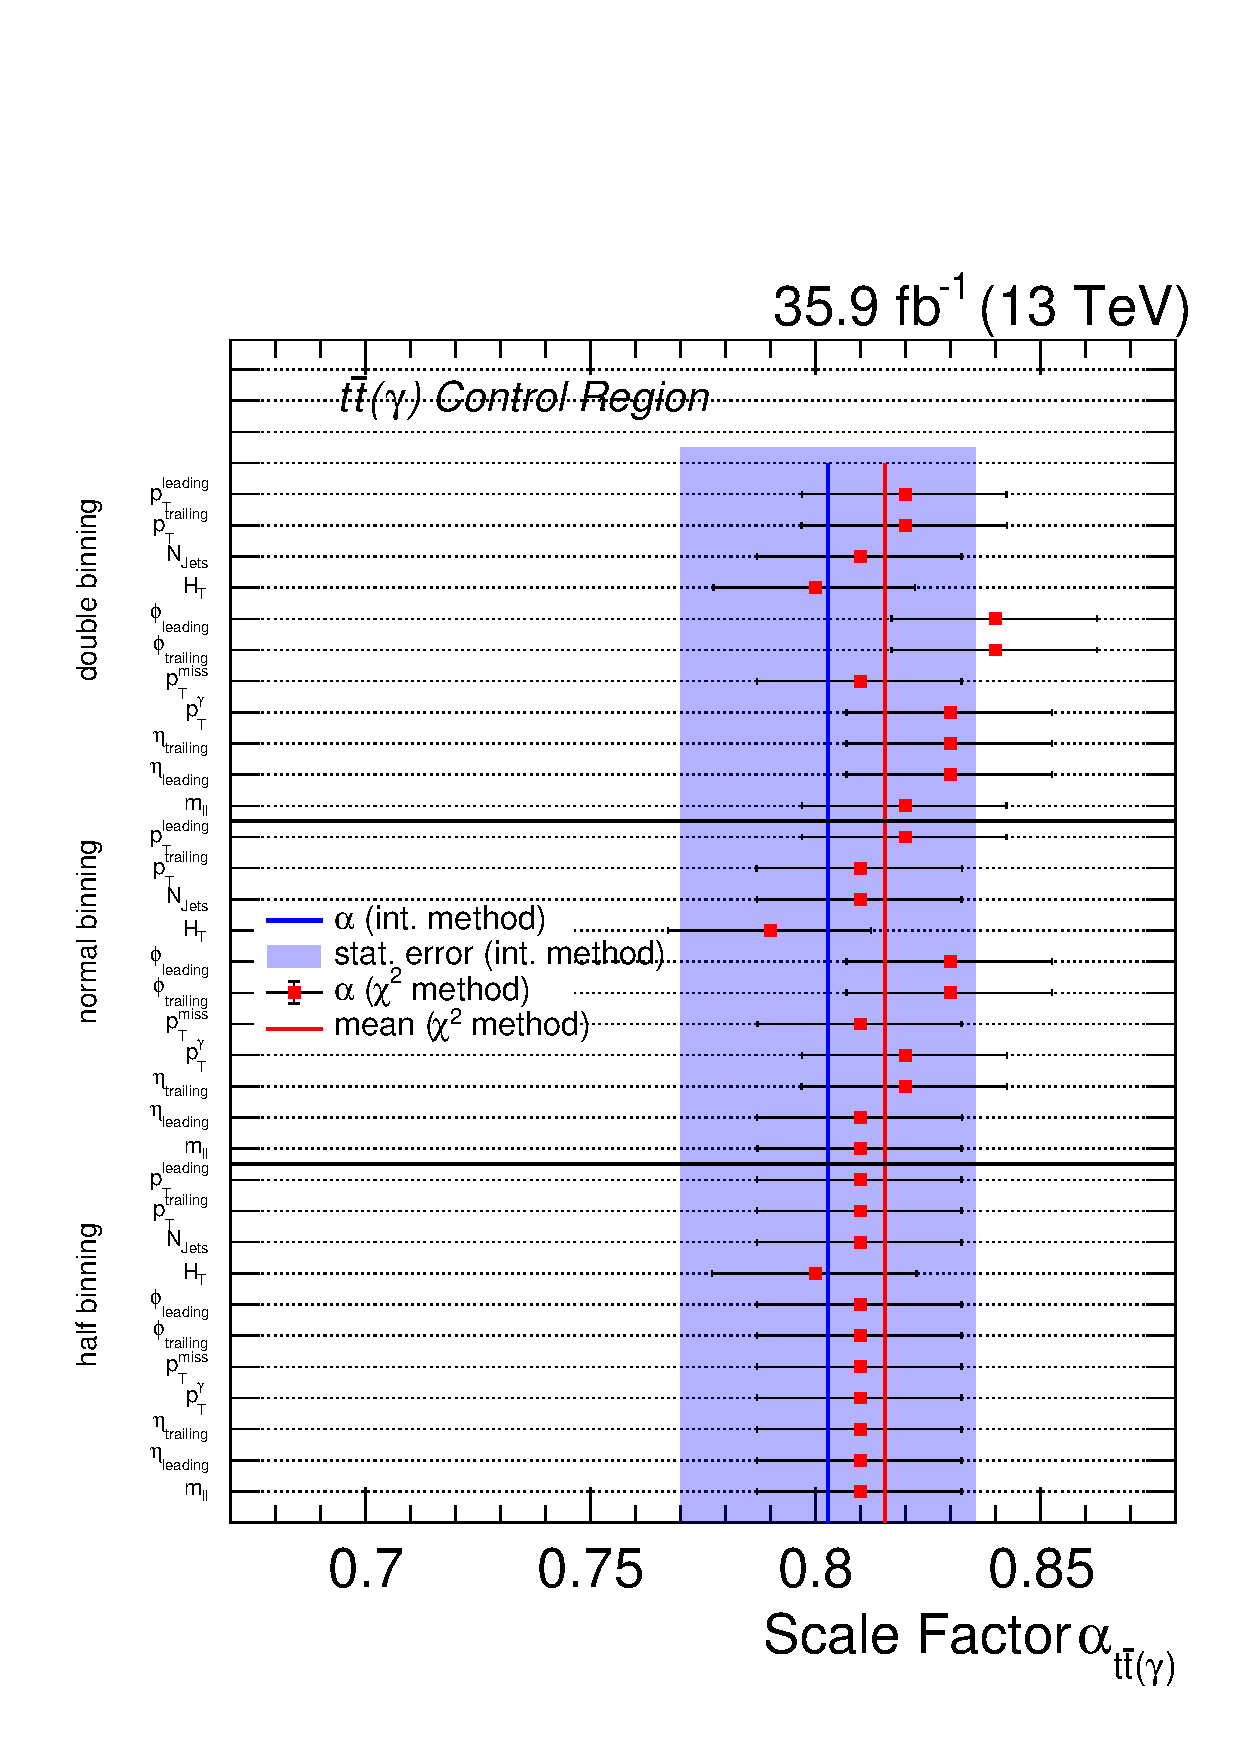
\includegraphics[width=\pairwidth]{figures/plots_CR/chi/TT_Compare}
 \caption{Example $\chi^2$-fit in the $\ttbar(\PGg)$ CR in the $\ptmiss$ distribution (left) with the polynomial fit. All fit results compared with the SF obtained from the integral method in different binnings and variables (right).}
 \label{fig:chiTT}
\end{figure}

\subsubsection*{Further studies}
Since the $\ttbar(\PGg)$ background is the most dominating one, further studies are performed in which the underlying MC simulation samples and their combination are examined. Different overlap removal procedures, see \refSec{sec:overlap}, and different available cross sections are used, while the fit procedure itself is varied. In addition, available corrections to improve the modeling of jet radiation in the initial state, and corrections to enhance the description of the top quark $\pt$ distribution, that are used both to correct the LO samples and the samples that are generated with \POWHEG (see~\refSec{sec:Simulation}), are applied in different combinations. The used fit methods include a $\chi^2$-template fit, where the ratio between the fractions of the $\ttbar$ and $\ttbar\PGg$ simulation is left free as an additional parameter, and a fit where only the $\ttbar\PGg$ simulation is made use of. The additional corrections to improve the modeling of the top quark $\pt$ distribution and the initial state jet radiation are observed to be unnecessary, because the modeling of the related distributions, \ie the jet multiplicity and the lepton $\pt$ distributions, is already in agreement with data in the standalone simulation. Using only the $\ttbar\PGg$ simulation yields the best agreement between simulated and observed shape, but is unphysical due to the missing $\ttbar$ process. For this reason, also the template fit method gives rise to similar results, since in the fit the $\ttbar\PGg$ sample has the highest impact due to the good shape agreement. Therefore, this approach is discarded, too. Eventually, no substantial differences are observed, and the best performance and stability is provided by the approach explained above.

\subsection{$\PW\PZ$ diboson production}
The diboson production of $\PW\PZ$ pairs is the second important background contribution for this analysis. It is also tuned to agree with the measurement in the $\PW\PZ$ CR, while the SF $\alpha_{\PW\PZ}$ is calculated with the integral method. The expected purity of selected $\PW\PZ$ events in this CR is about $84\%$.
% \begin{table}[tbp]
%  \centering
%  \caption{Yields in the $\PW\PZ$ CR for the pure simulation and measured data.}
%  \label{tab:CRWZ}
%  \begin{tabular}{llll}
%   process  & raw simulation & simulation & data                  \\\hline
%   $\PW\PZ$ & 113744         & 895.74     &                       \\\hline\hline
%   sum      & 113744         & 895.74     & \multirow{2}{*}{1193} \\
%   other    & 93914          & 173.47     &
%  \end{tabular}
% \end{table}
% The agreement beforehand is also very good, considering this background is a higher order process and is therefore simulated at NLO, see \refSec{sec:Simulation}, which includes several complicated effects the event generator needs to handle properly.
The SF $\alpha_{\PW\PZ}$ is determined to be
\begin{equation}\label{eq:AlphaWZ}
 \alpha_{\PW\PZ}=1.14 \pm 0.04 (stat.) [\hat{=}3.2\%].
\end{equation}
Higher order effects can lead to larger cross sections as calculated within the NLO simulation, thus it is not unexpected to obtain a SF varying $\approx12\%$ from unity. Resulting distributions of the description of the $\ptmiss$ and $\mtTwo$ variables are shown in \refFig{fig:CRWZ}. As can be seen, the predicted shape is in consistency over the whole range with the observed data, also in the high $\ptmiss$ and $\mtTwo$ regime. This is further confirmed by the additional cross checks, that are also realized in the $\ttbar(\PGg)$ CR described above. The KS-values close to one strengthen the trust in the background estimation method.
% The comparison plots for other distributions can be found in the appendix in \refFig{fig:app_}.
\begin{figure}[tbp]
 \centering
 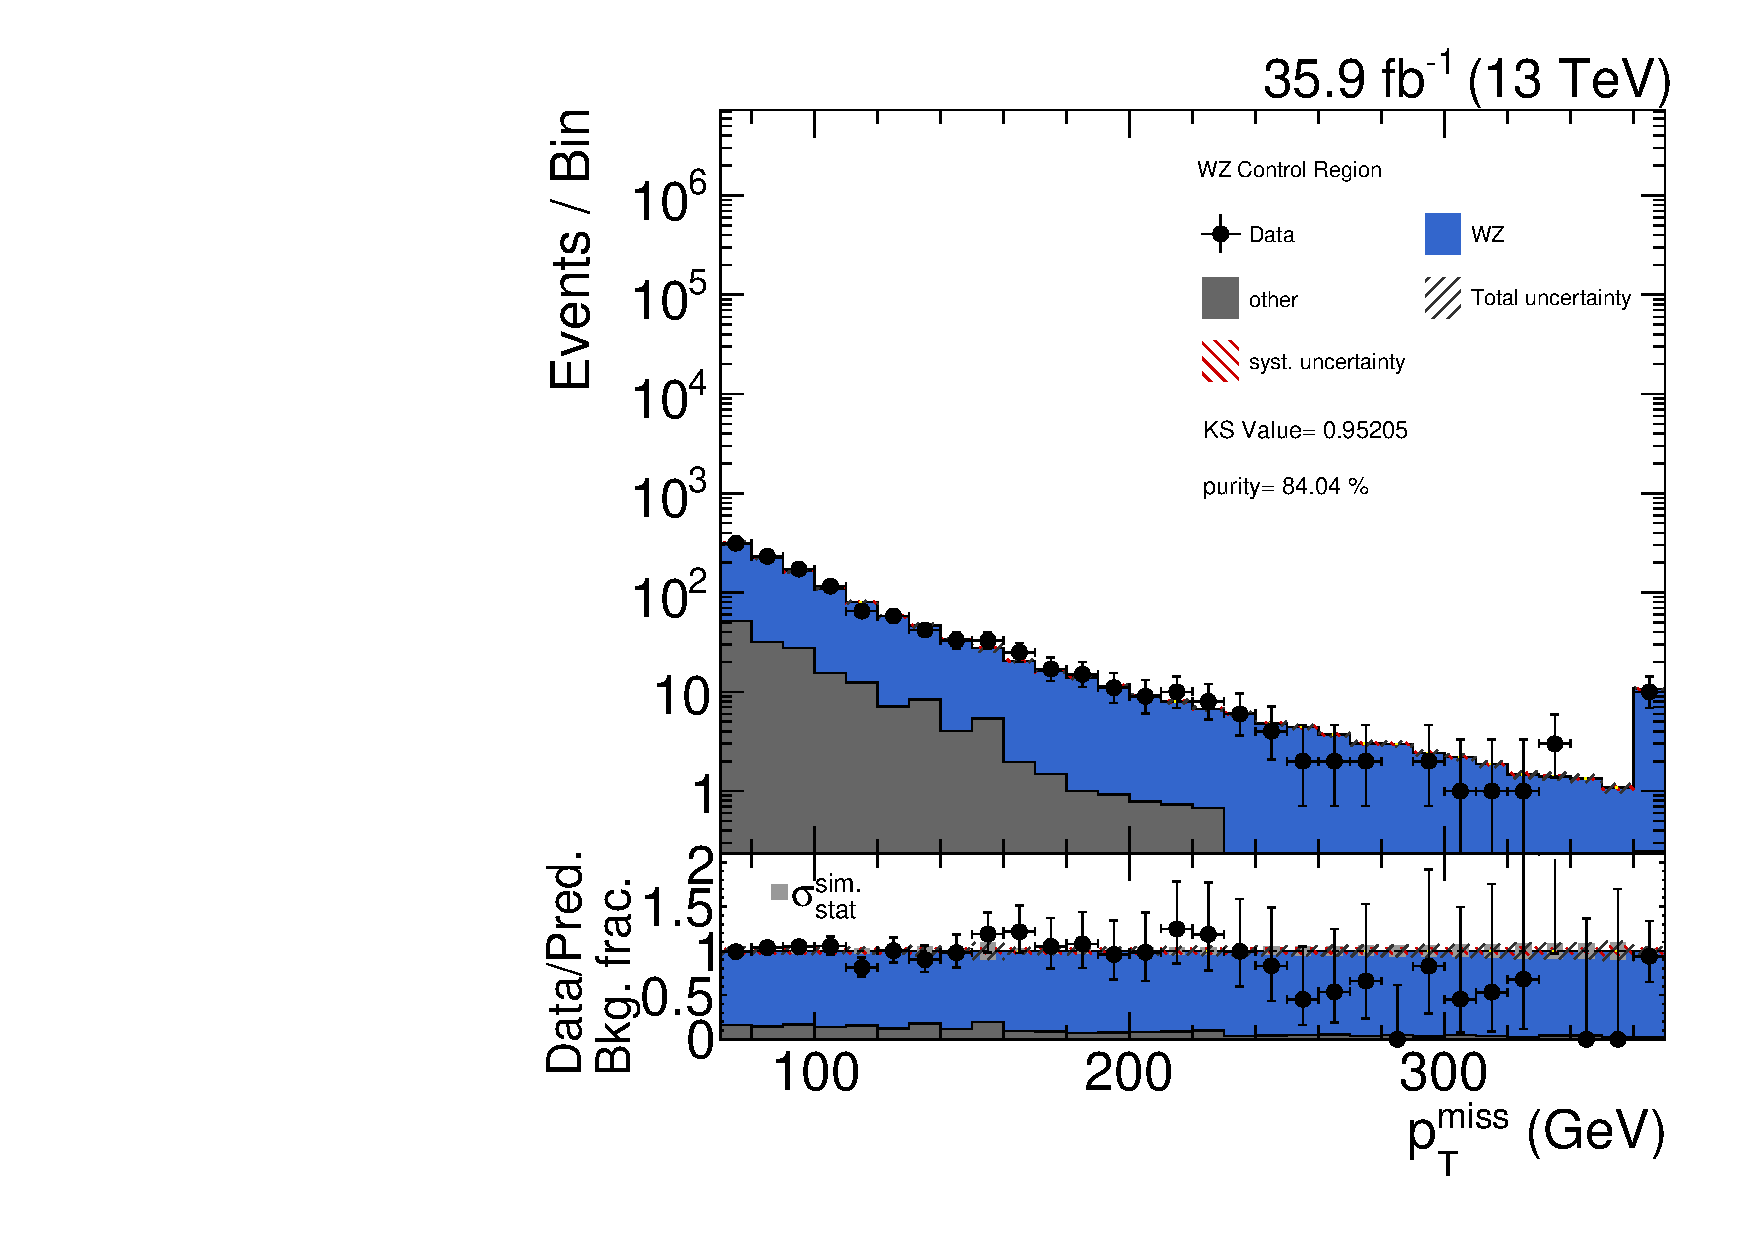
\includegraphics[width=\pairwidth]{figures/plots_CR_wz/CRWZ_LL_nom_met_log}
 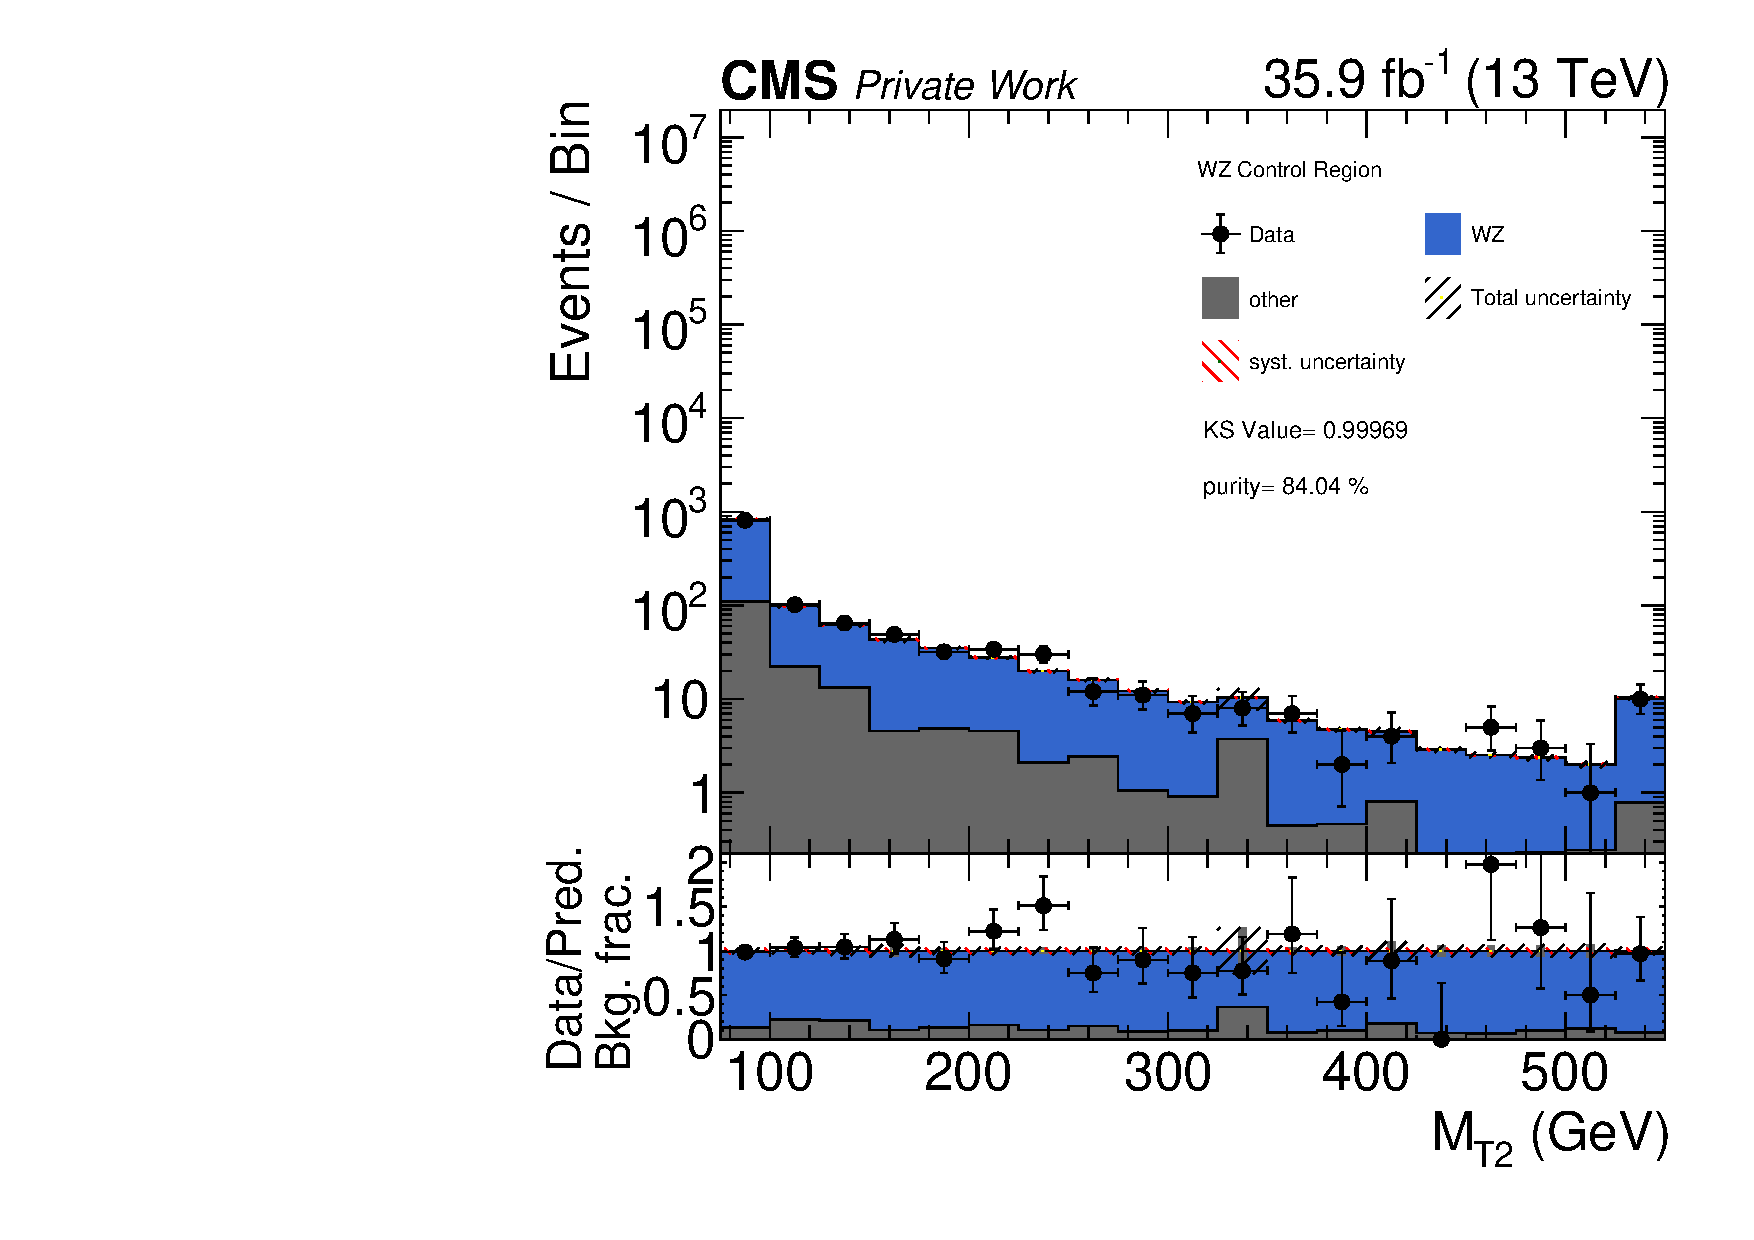
\includegraphics[width=\pairwidth]{figures/plots_CR_wz/CRWZ_LL_nom_mt2_log}
 \caption{Comparisons between data and rescaled simulation in the $\PW\PZ$ CR in the $\ptmiss$ and $\mtTwo$ distribution. Below each plot, a ratio between data and prediction is shown. The uncertainty bands correspond to the systematic (rand) and total uncertainty (gray). In addition, in the ratio plot the relative composition of the backgrounds is visualized. KS-values for the performed Kolmogorov-Smirnov test and the selection purity are also quoted.}
 \label{fig:CRWZ}
\end{figure}
The $\chi^2$-fit studies lead to the same outcome as can be seen in \refFig{fig:chiWZ} right. Each individual $\chi^2$-fit seems to behave properly, see \refFig{fig:chiWZ} (left) for an example in the $\ptmiss$ distribution.

\begin{figure}[tbp]
 \centering
 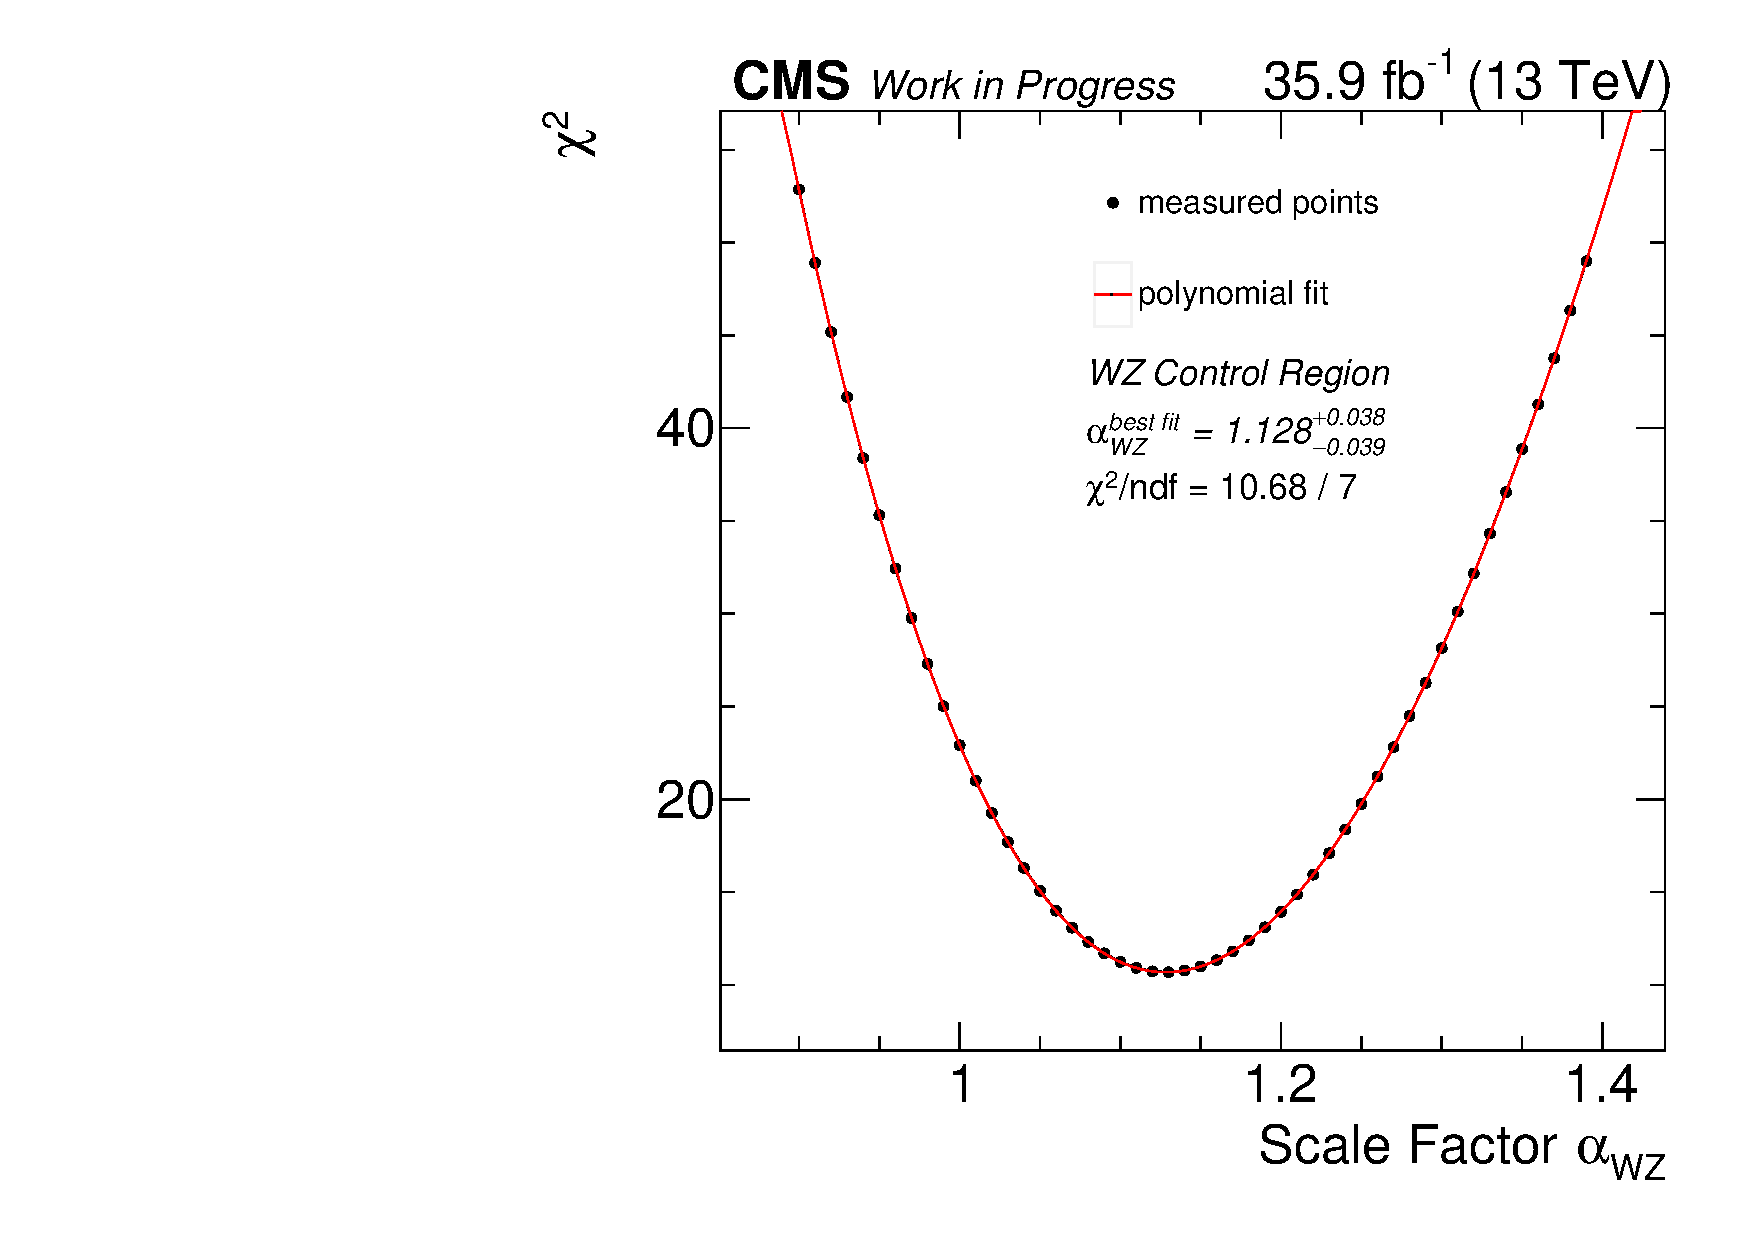
\includegraphics[width=\pairwidth]{figures/plots_CR/chi/WZ_met}
 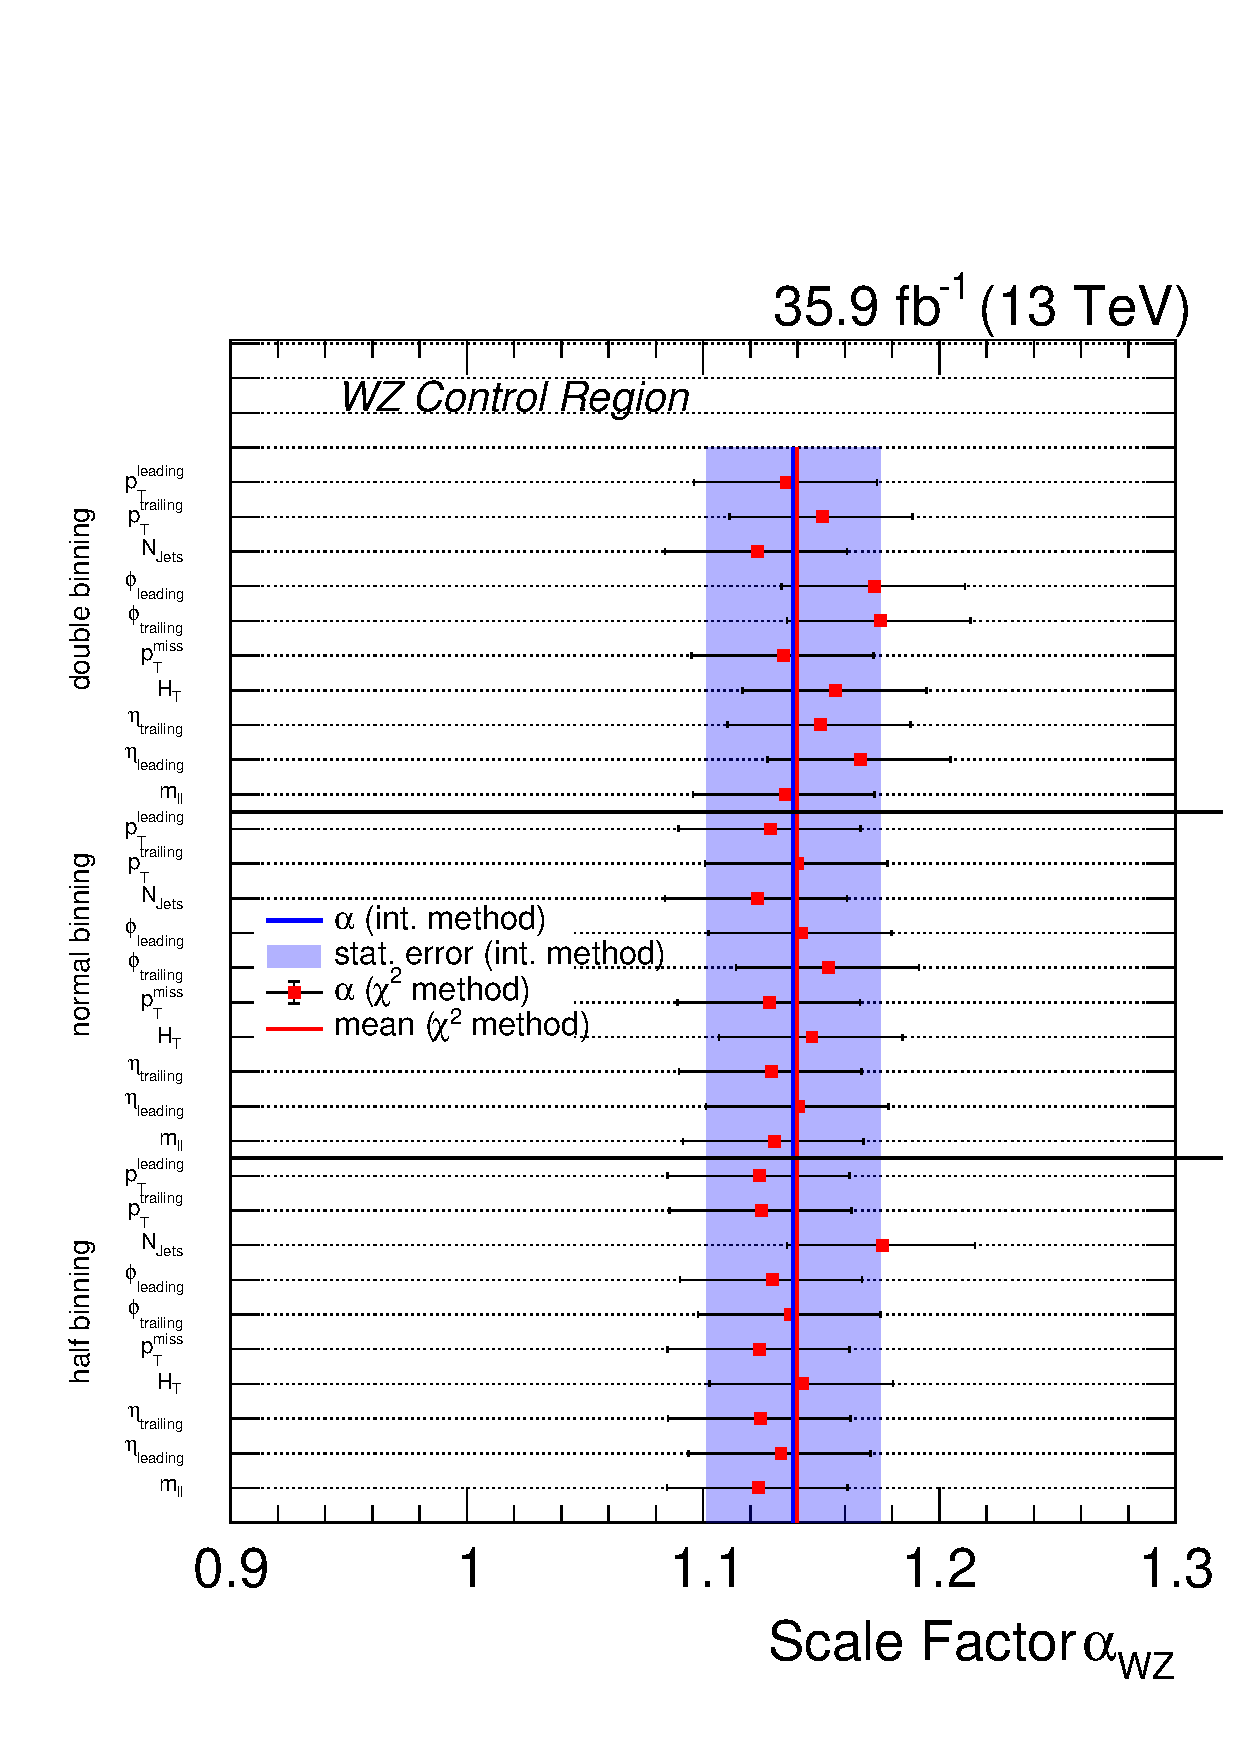
\includegraphics[width=\pairwidth]{figures/plots_CR/chi/WZ_Compare}
 \caption{Example $\chi^2$-fit in the $\PW\PZ$ CR in the $\ptmiss$ distribution (left) with the polynomial fit. All fit results compared with the SF obtained from the integral method in different binnings and variables (right).}
 \label{fig:chiWZ}
\end{figure}




\subsection{$\PZ\PZ$ diboson production}
The third biggest background contribution is $\PZ\PZ$ diboson production, where both Z bosons decay leptonically, one to charged leptons such as electrons or muons, and the other one to neutrinos. To simplify the construction of a dedicated CR, as explained in \refSec{sec:CR}, the simulation procedure is exploitet. Since the simulation of the events is the same for both charged leptons and neutrinos for the Z boson decays due to the identical generator, only the detector response differs. Therefore, $\PZ\PZ$ can be well estimated in a four lepton CR. A pure selection of $\PZ\PZ$ events can be established, although the statistics in data is quite low due to small cross section and the low branching fraction for the $\Z\to\ell\ell$ decay. The selection purity is nearly $100\%$.
% Event counts are quoted in \refTab{tab:CRZZ}, with a selection purity of nearly $100\%$.
% \begin{table}[tbp]
%  \centering
%  \caption{Yields in the $\PZ\PZ$ CR for the pure simulation and measured data.}
%  \label{tab:CRZZ}
%  \begin{tabular}{llll}
%
%   process                 & raw simulation & simulation & data                 \\\hline
%   $\PZ\PZ(\to2\ell2\Pgn)$ & 5              & 0.0005     &                      \\
%   $\PZ\PZ(\to4\ell)$      & 459221         & 226.94     &                      \\\hline\hline
%   sum                     & 459226         & 226.94     & \multirow{2}{*}{251} \\
%   other                   & 74             & 1.48       &
%  \end{tabular}
% \end{table}
With the integral method applied, the SF $\alpha_{\PZ\PZ}$ is given by
\begin{equation}\label{eq:AlphaZZ}
 \alpha_{\PZ\PZ}=1.109 \pm 0.064 (stat.) [\hat{=}5.74\%].
\end{equation}
Post-fit distributions in the $\ptmiss$ distribution and invariant dilepton mass distribution of the second Z boson can be found in \refFig{fig:CRZZ}. As mentioned, the precision is limited by the low statistics of the selected sample, but nevertheless is sufficient enough to establish a stable background prediction. The shapes agree well, as it is additionally indicated by the KS-values printed on the plots. The properties of the $\PZ\PZ\to4\ell$ process does not allow to study the prediction in the high $\ptmiss$ regime, since only nongenuine $\ptmiss$ is produced. However, based on the agreement of distributions of the third and fourth leptons, such as $m_{\ell_3\ell_4}$, and the agreement of the description of nongenuine $\ptmiss$, the agreement of $\ptmiss$ in the $\PZ\PZ\to2\ell2\PGn$ background can be assumed.
\begin{figure}[tbp]
 \centering
 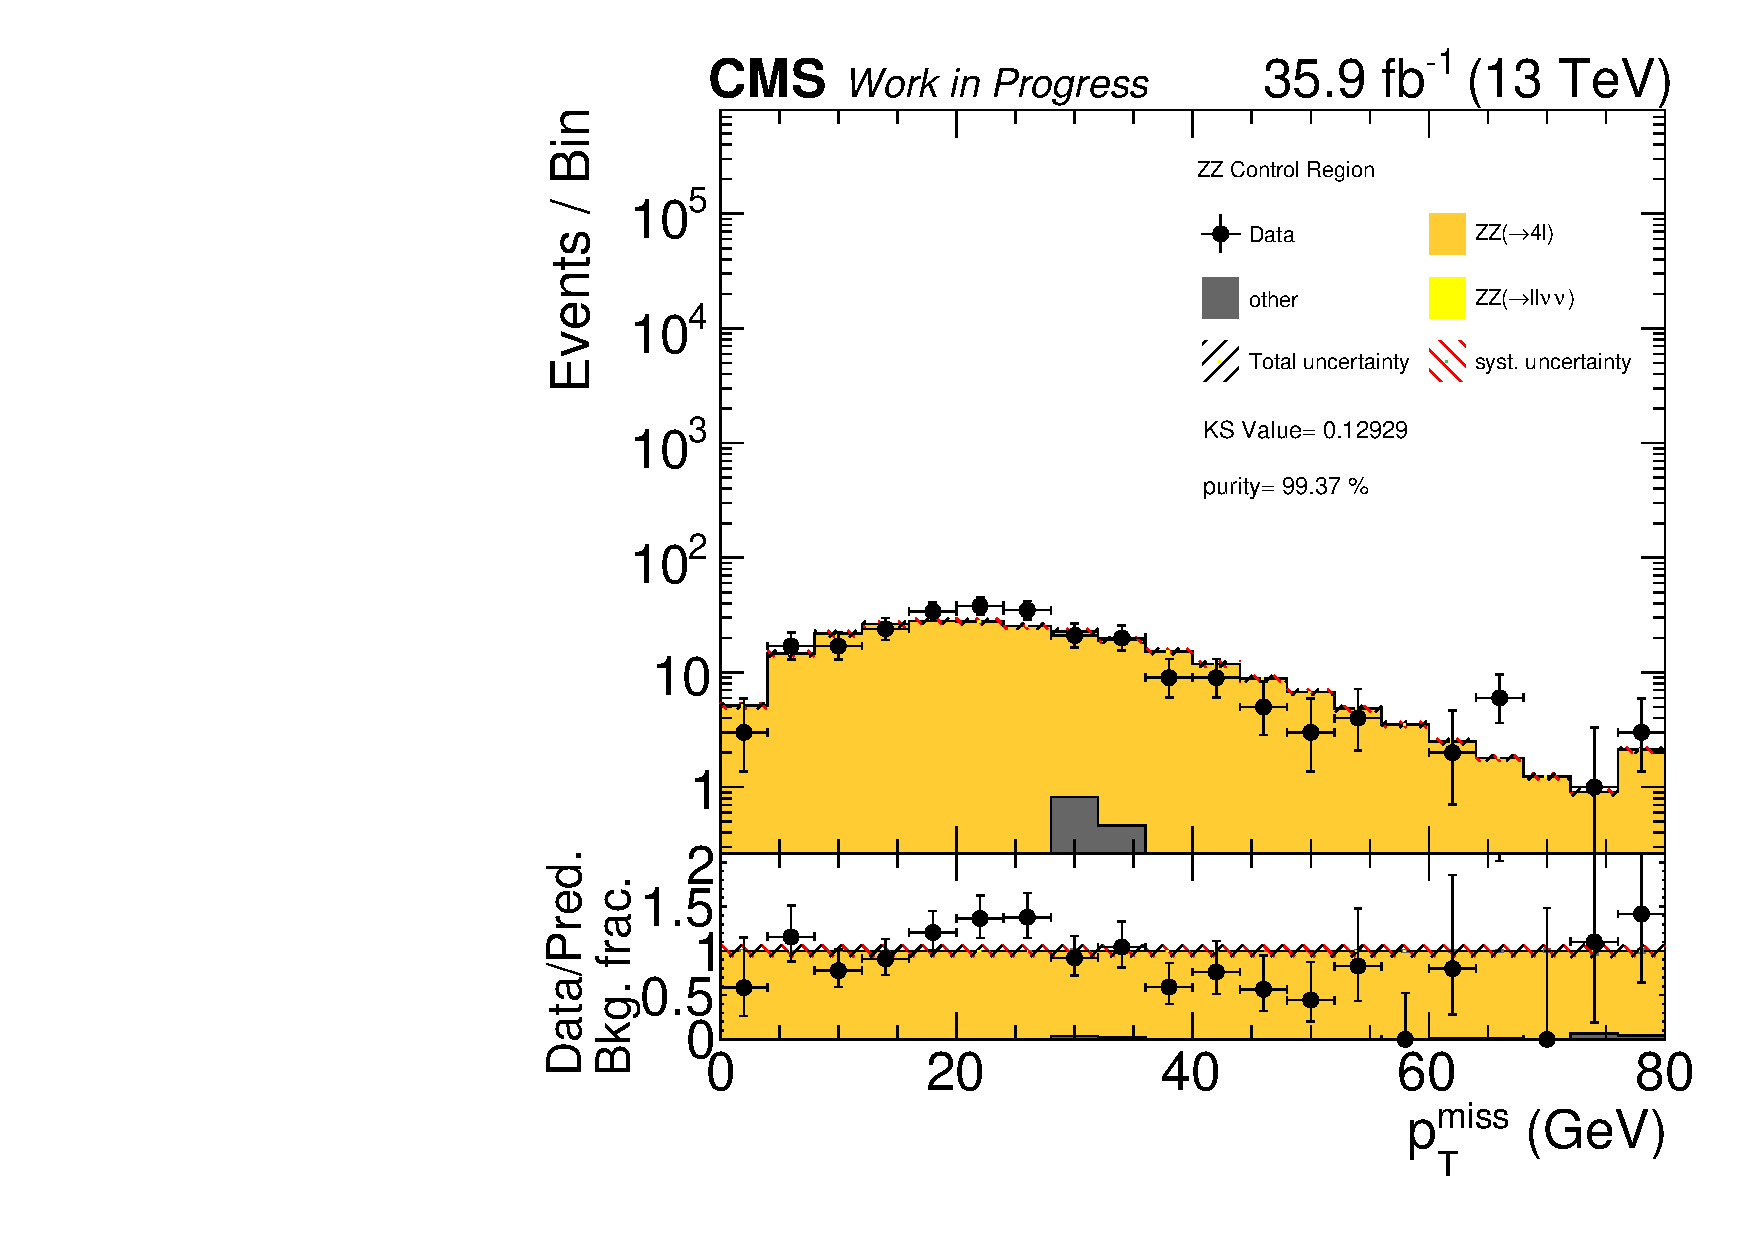
\includegraphics[width=\pairwidth]{figures/plots_CR_zz/CRZZ_LL_nom_met_log}
 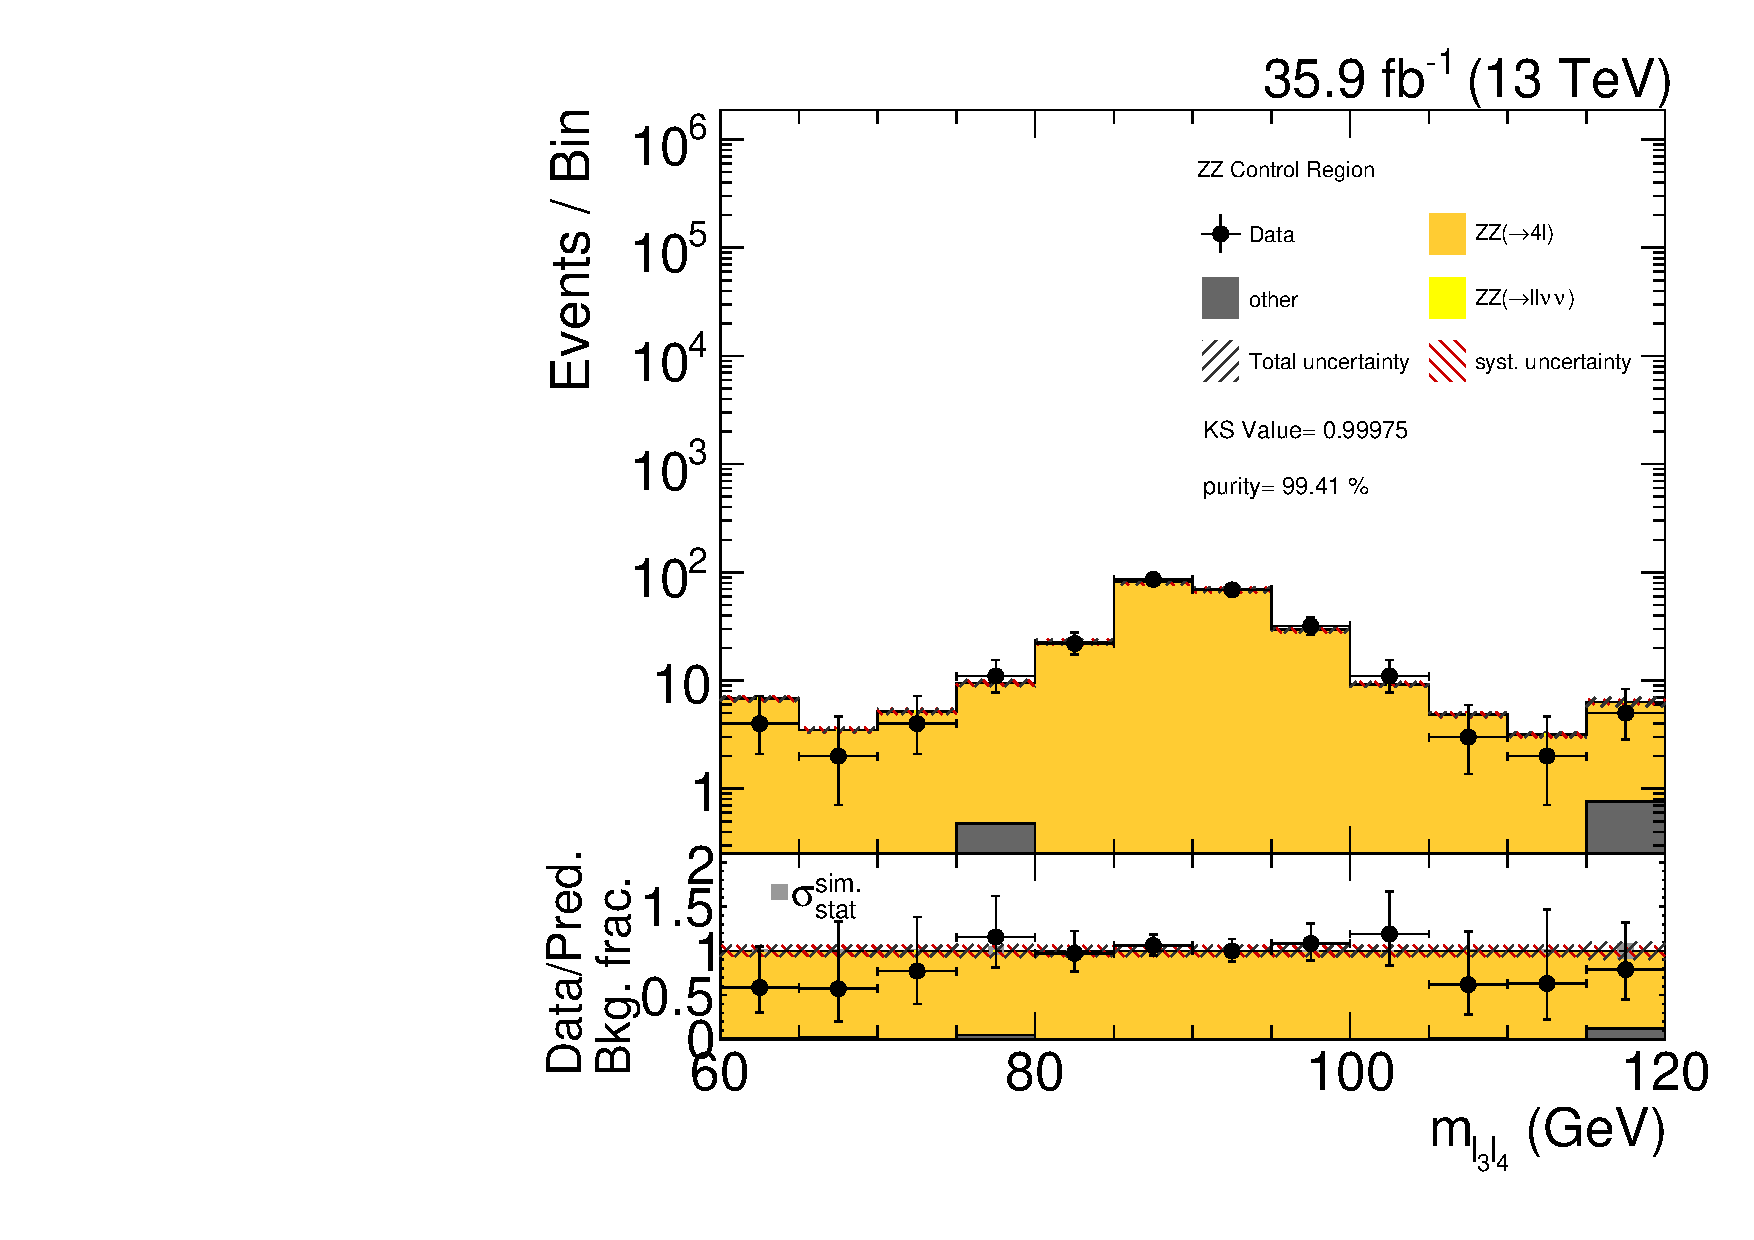
\includegraphics[width=\pairwidth]{figures/plots_CR_zz/CRZZ_LL_nom_m_ll2_log}
 \caption{Comparisons between data and rescaled simulation in the $\PZ\PZ$ CR in the $\ptmiss$ and $m_{\ell_3\ell_4}$ distribution. Below each plot, a ratio between data and prediction is shown. The uncertainty bands correspond to the systematic (red) and total uncertainty (gray). In addition, in the ratio plot the relative composition of the backgrounds is visualized. KS-values for the performed Kolmogorov-Smirnov test and the selection purity are also quoted.}
 \label{fig:CRZZ}
\end{figure}
The $\chi^2$-fit studies, see \refFig{fig:chiZZ}, are performed as for the other three background estimations discussed above, and yield the same conclusion, although some fluctuations in the choice of the variable or binning are present due to the lower total event count in the observed data. All in all also this background estimation method is stable.
\begin{figure}[tbp]
 \centering
 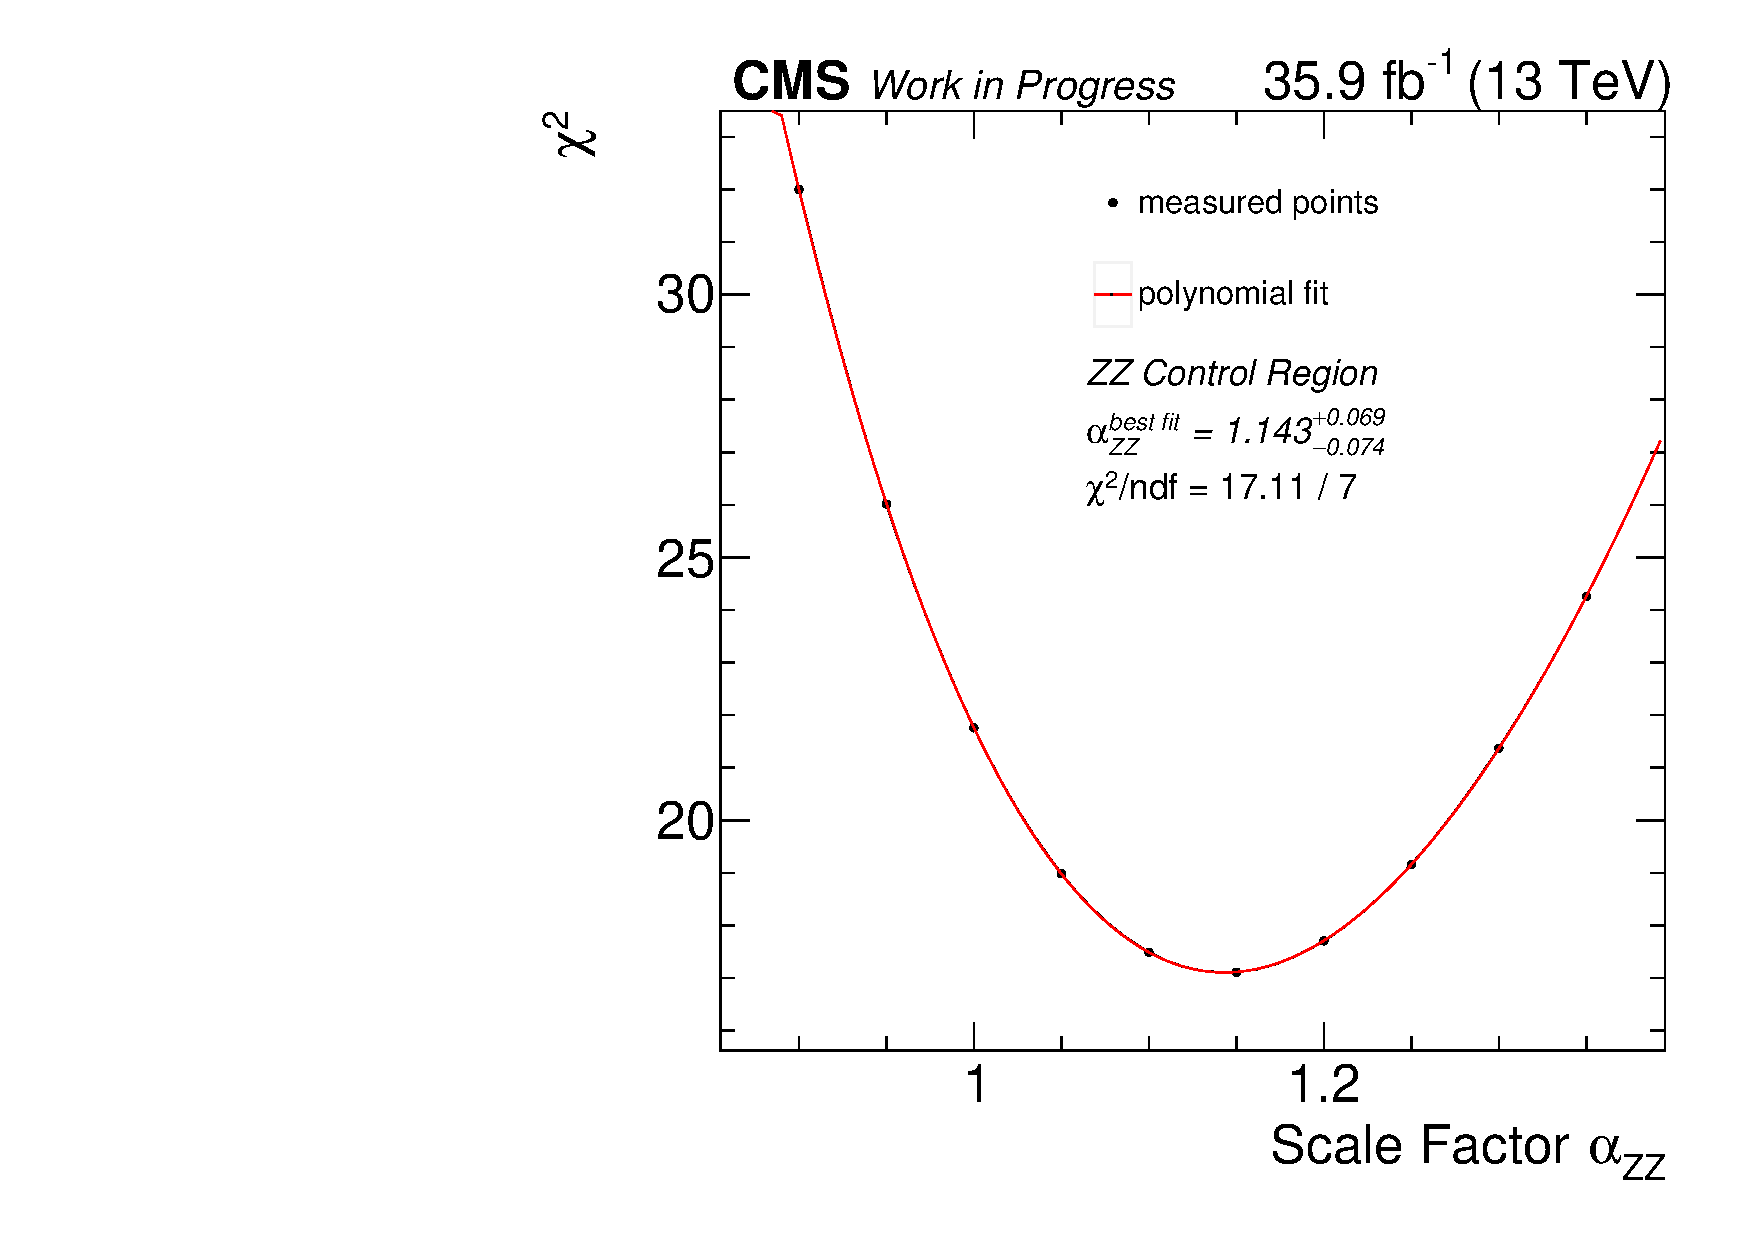
\includegraphics[width=\pairwidth]{figures/plots_CR/chi/ZZ_met}
 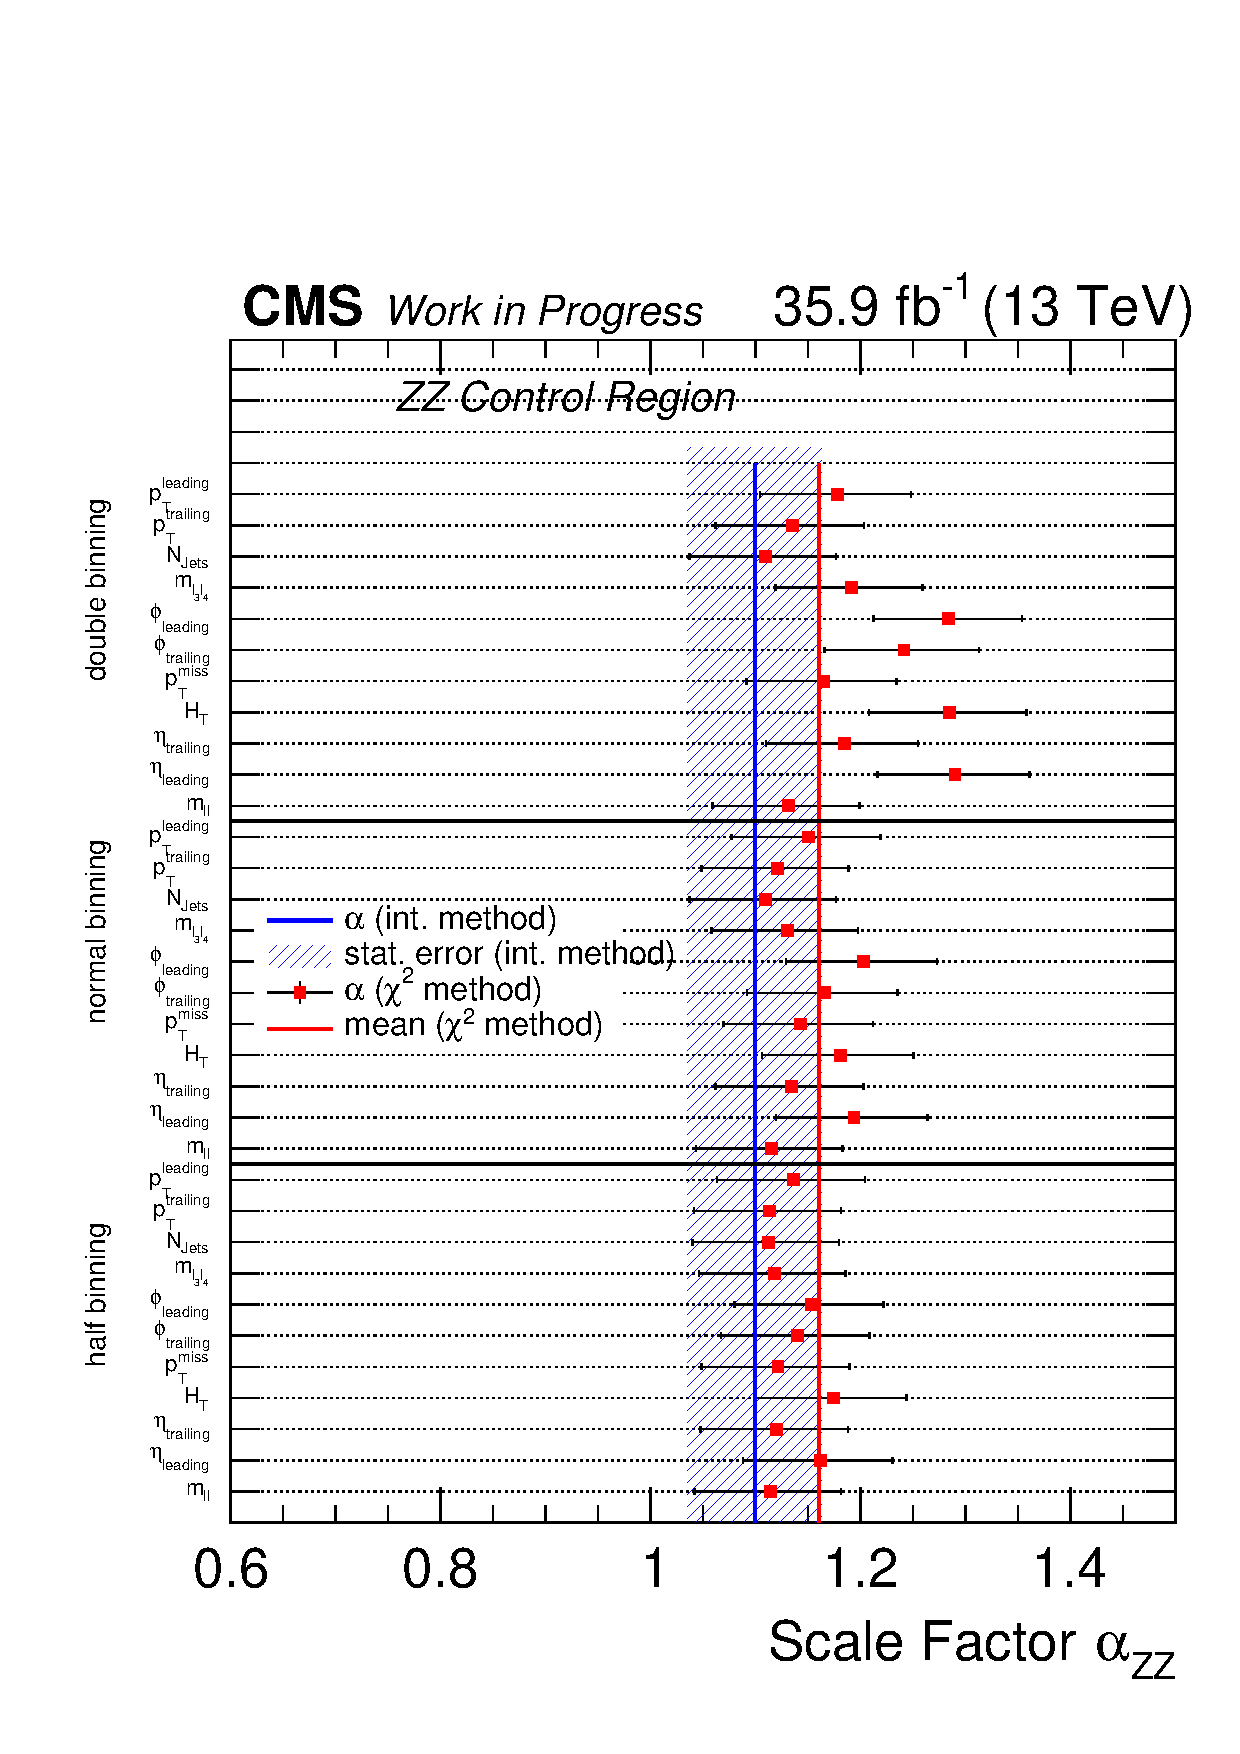
\includegraphics[width=\pairwidth]{figures/plots_CR/chi/ZZ_Compare}
 \caption{Example $\chi^2$-fit in the $\PZ\PZ$ CR in the $\ptmiss$ distribution (left) with the polynomial fit. All fit results compared with the SF obtained from the integral method in different binnings and variables (right).}
 \label{fig:chiZZ}
\end{figure}

\subsection{Drell-Yan and $\PZ\PGg$ production}
Although contribution from the Drell-Yan and $\PZ\PGg$ backgrounds is small in the two SR bins, its contribution is the fourth largest. As in the case of the $\ttbar(\PGg)$ background, it is composed of two major parts, the Drell-Yan process, where quarks annihilate to off-shell photons or Z bosons and generate leptons in their decays, and the diboson production of $\PZ\PGg$. The integral method as explained above is used to determine the SF $\alpha_{DY/\PZ(\PGg)}$ in the dedicated CR defined in \refSec{sec:CR}.
% The relevant event yields are quoted in \refTab{tab:CRDY}, and t
The resulting SF is stated in \refEq{eq:AlphaDY}. With a purity of about $99\%$, and a large total event count, a precise SF determination is feasible, as can be concluded also from the small statistical uncertainty of around $1\%$. The agreement between simulation and data is very good even before application of $\alpha_{DY/\PZ(\PGg)}$, since the SF equals nearly unity. The post-scaling distributions of $\ptmiss$ and $\mtTwo$ are shown in \refFig{fig:CRDY}. They show overall a good agreement, only in the high $\mtTwo$ region there are some fluctuations due to the limited statistics being present both in data and simulation.
% Further distributions are investigated, that can be found in the appendix in \refFig{fig_app}.
Most of the KS-values indicate a very good matching between predicted and observed shape, albeit the Kolmogorov-Smirnov test provides a very small KS value for the consistency between the $\ptmiss$ distributions. This is mainly due to the high statistics in data and therefore a higher absolute discrepancy, in contradiction to the lower statistics in simulation, leading to larger fluctuations. These discrepancy is also visible in the ratio in the bottom panel of the plot, but is consistent with the shown total uncertainty.\\
% \begin{table}[tbp]
%  \centering
%  \caption{Yields in the DY/$\PZ(\PGg)$ CR for the pure simulation and measured data.}
%  \label{tab:CRDY}
%  \begin{tabular}{llll}
%
%   process   & raw simulation & simulation & data                   \\\hline
%   Drell-Yan & 11710          & 13008.53   &                        \\
%   $\PZ\PGg$ & 170161         & 22692.88   &                        \\\hline\hline
%   sum       & 181871         & 35701.41   & \multirow{2}{*}{38419} \\
%   other     & 87337          & 377.02     &
%  \end{tabular}
% \end{table}
\begin{equation}\label{eq:AlphaDY}
 \alpha_{DY/\PZ(\PGg)}=1.066 \pm 0.001 (stat.) [\hat{=}0.87\%].
\end{equation}

\begin{figure}[tbp]
 \centering
 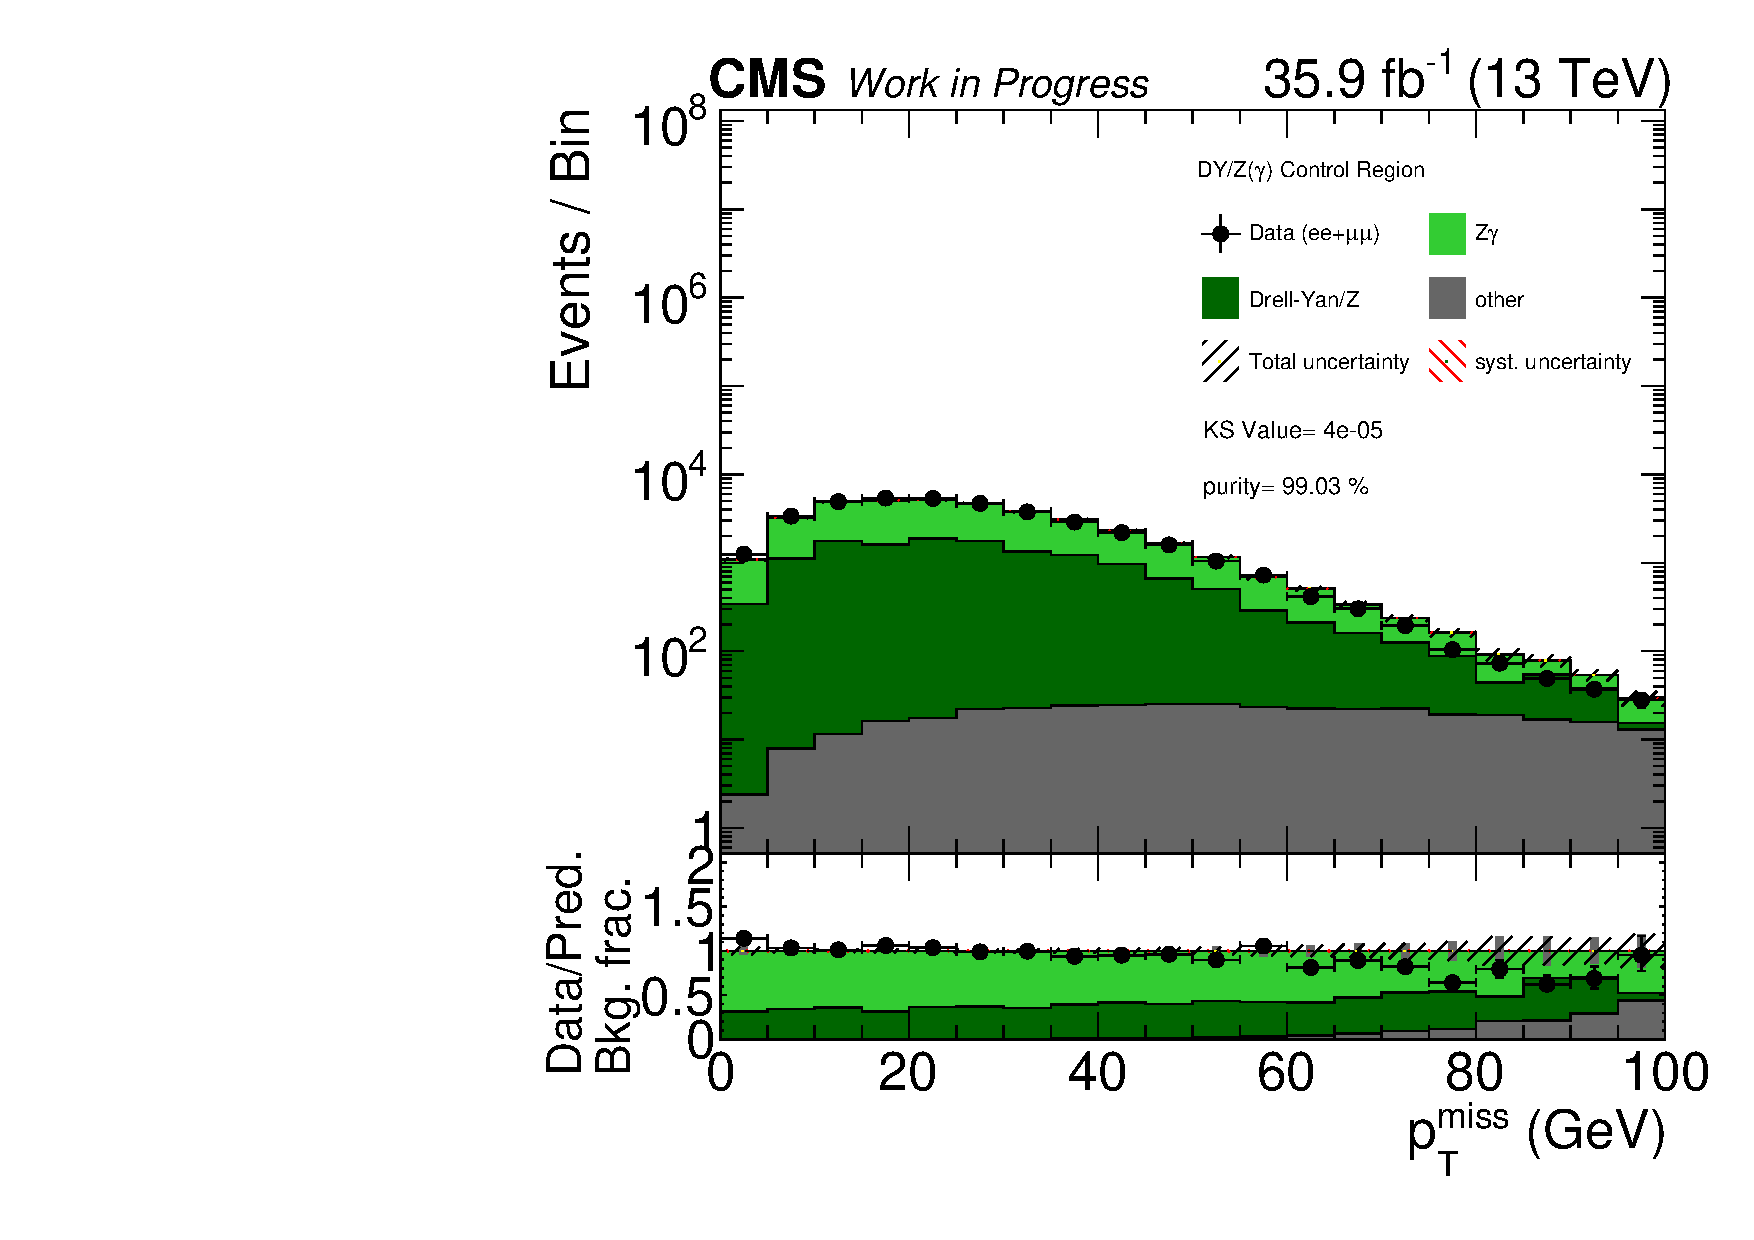
\includegraphics[width=\pairwidth]{figures/plots_CR_dy/CRDY_LL_nom_met_log}
 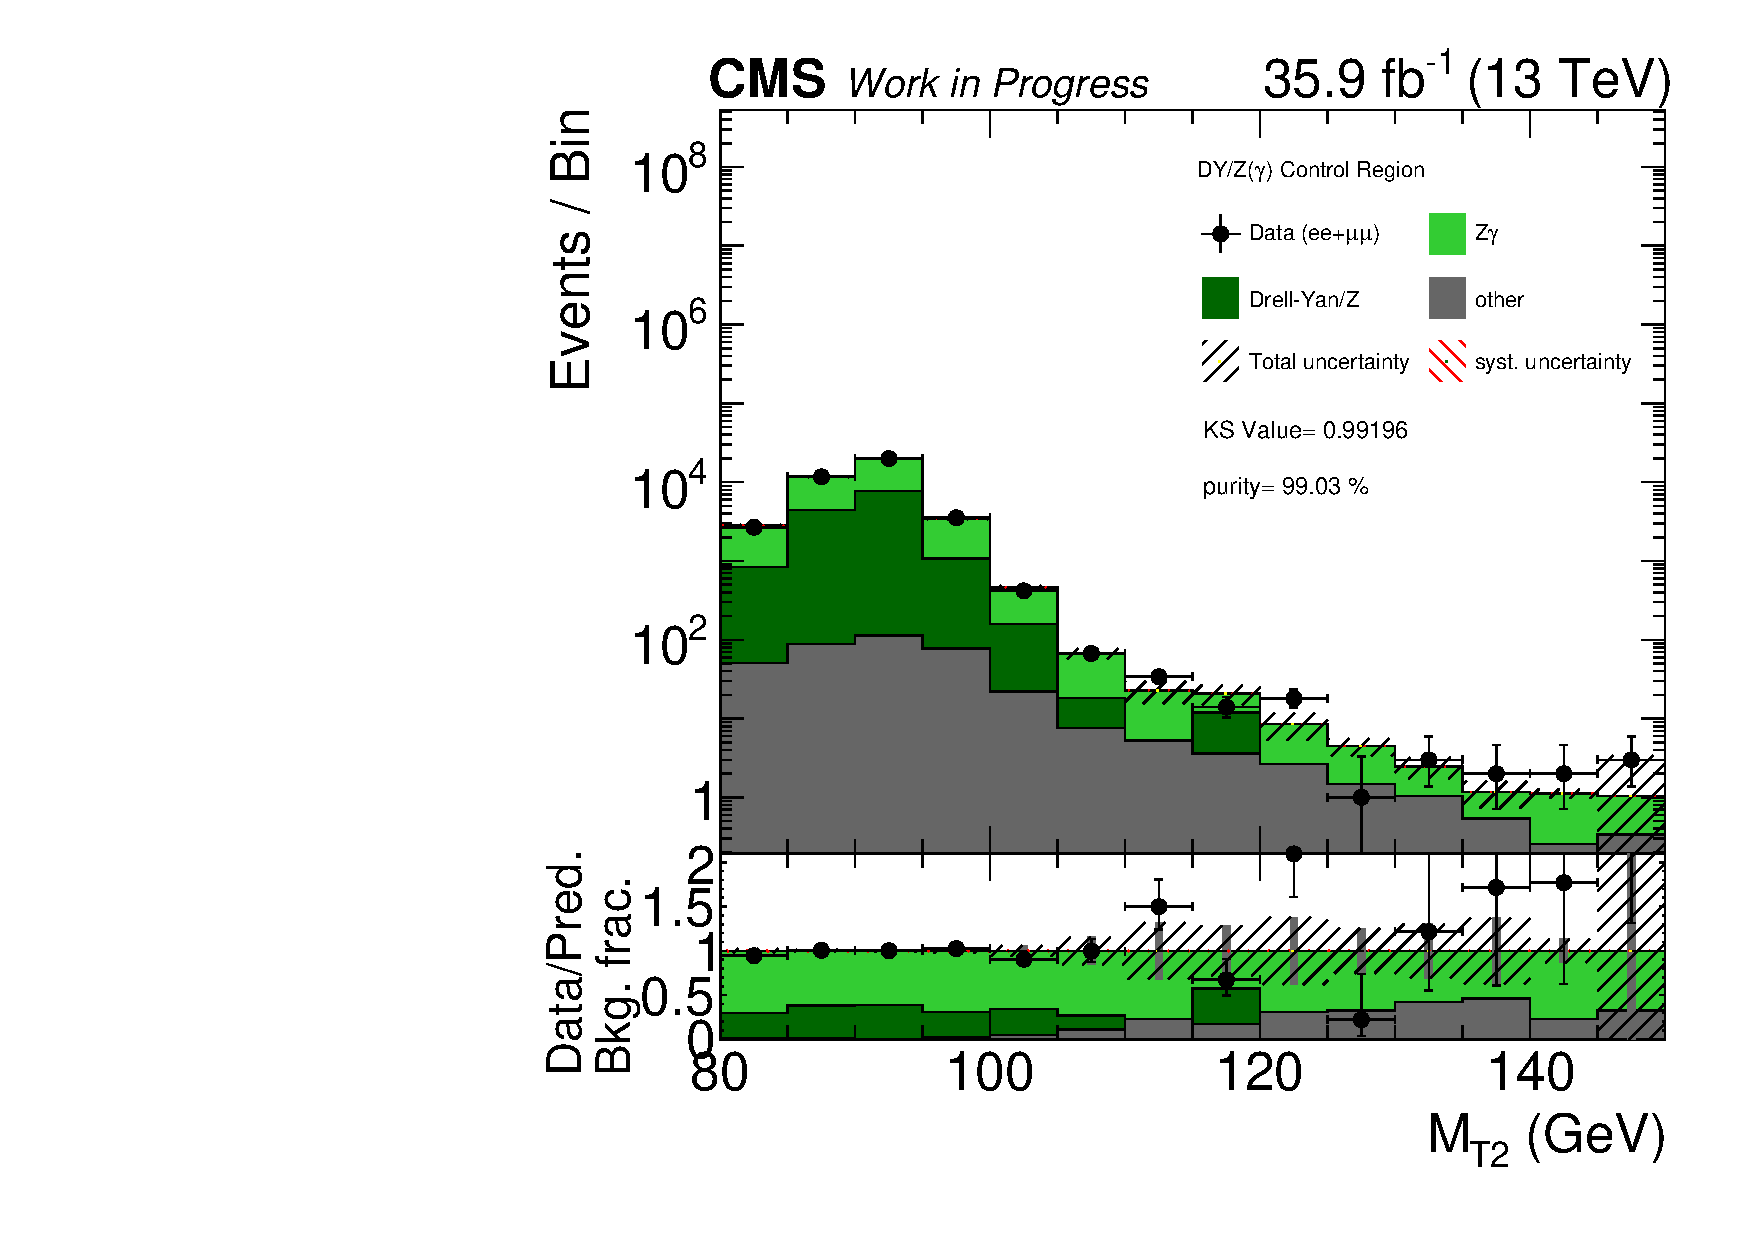
\includegraphics[width=\pairwidth]{figures/plots_CR_dy/CRDY_LL_nom_mt2_log}
 \caption{Comparisons between data and rescaled simulation in the DY/$\PZ(\PGg)$ CR in the $\ptmiss$ and $\mtTwo$ distribution. Below each plot, a ratio between data and prediction is shown. The uncertainty bands correspond to the systematic (red) and total uncertainty (gray). In addition, in the ratio plot the relative composition of the backgrounds is visualized. KS-values for the performed Kolmogorov-Smirnov test and the selection purity are also quoted.}
 \label{fig:CRDY}
\end{figure}
The $\chi^2$-fit studies, shown in \refFig{fig:chiDY} together with an example fit in the $\ptmiss$ distribution, show good agreement over all variations.

\begin{figure}[tbp]
 \centering
 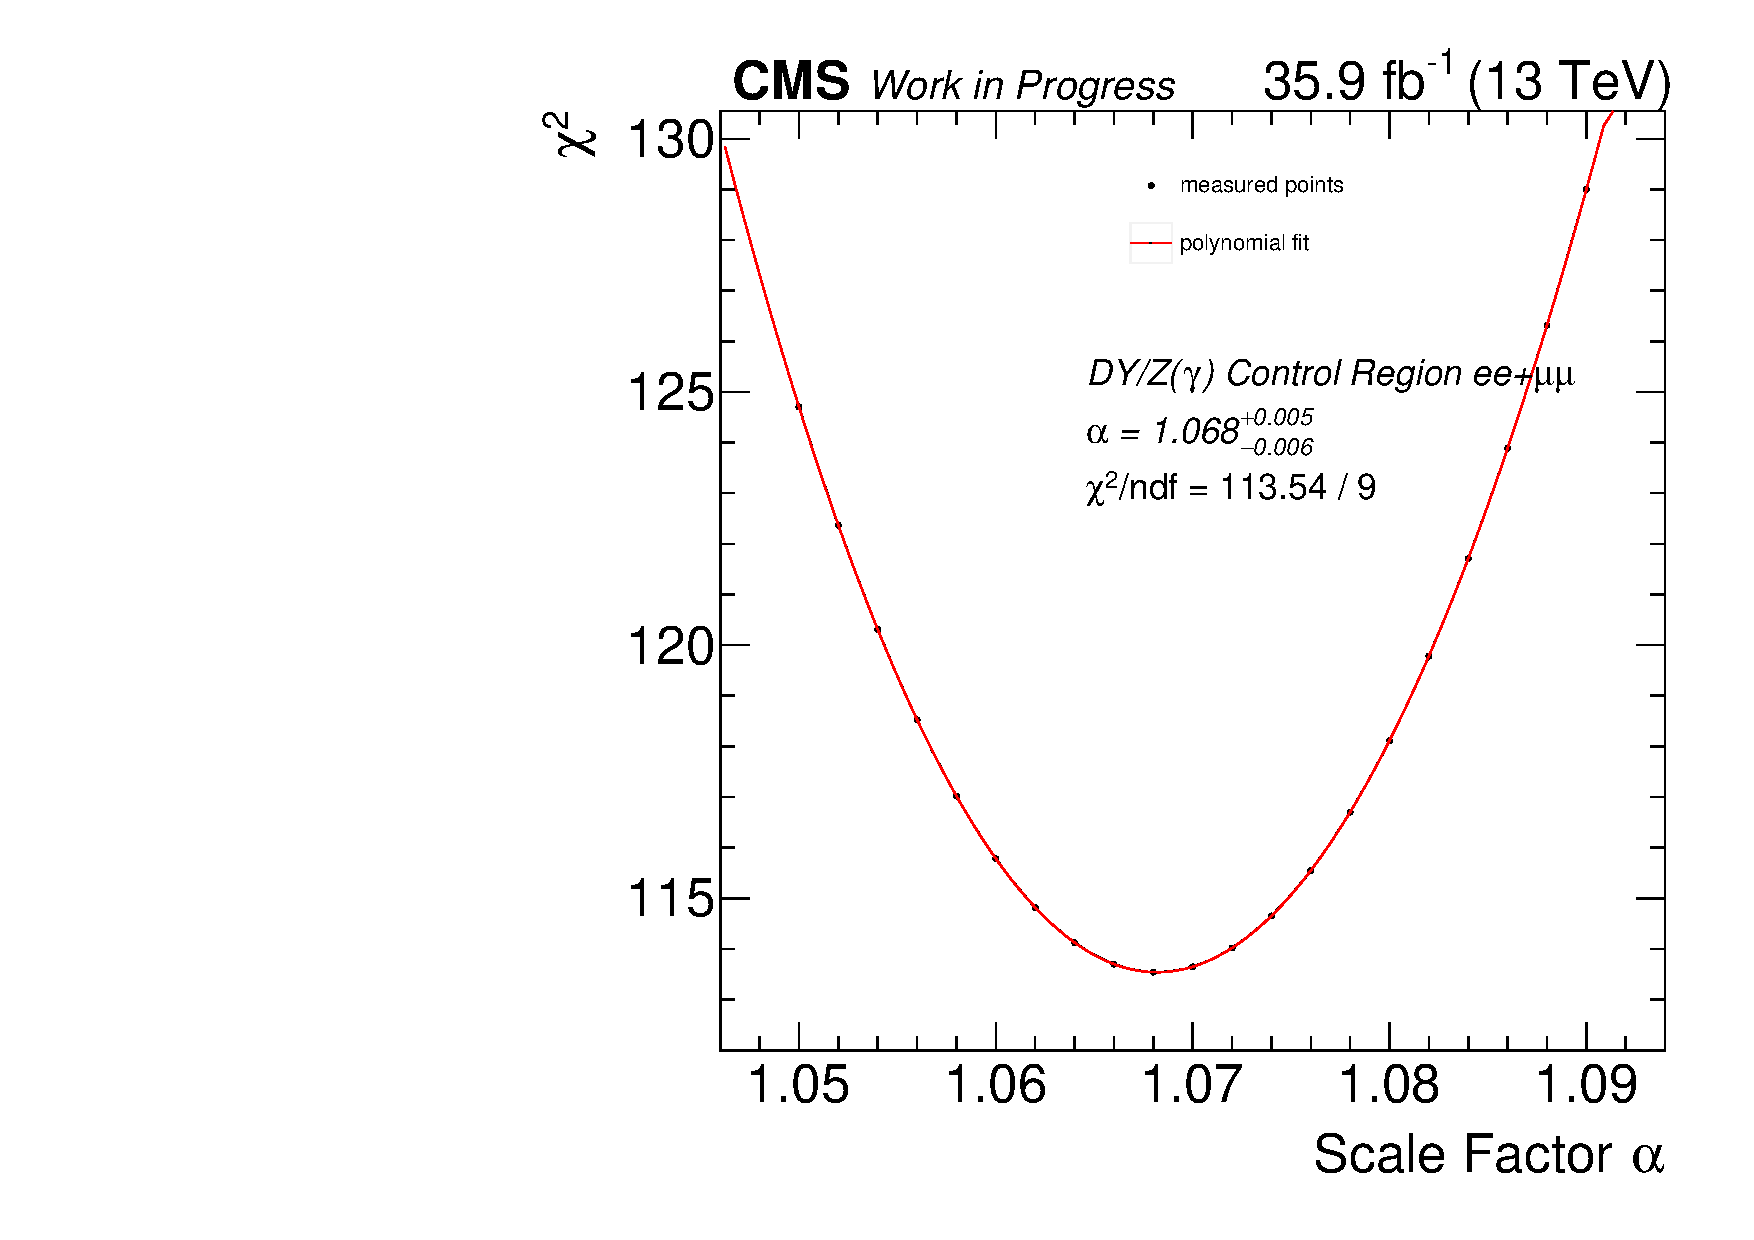
\includegraphics[width=\pairwidth]{figures/plots_CR/chi/DY_LL_met}
 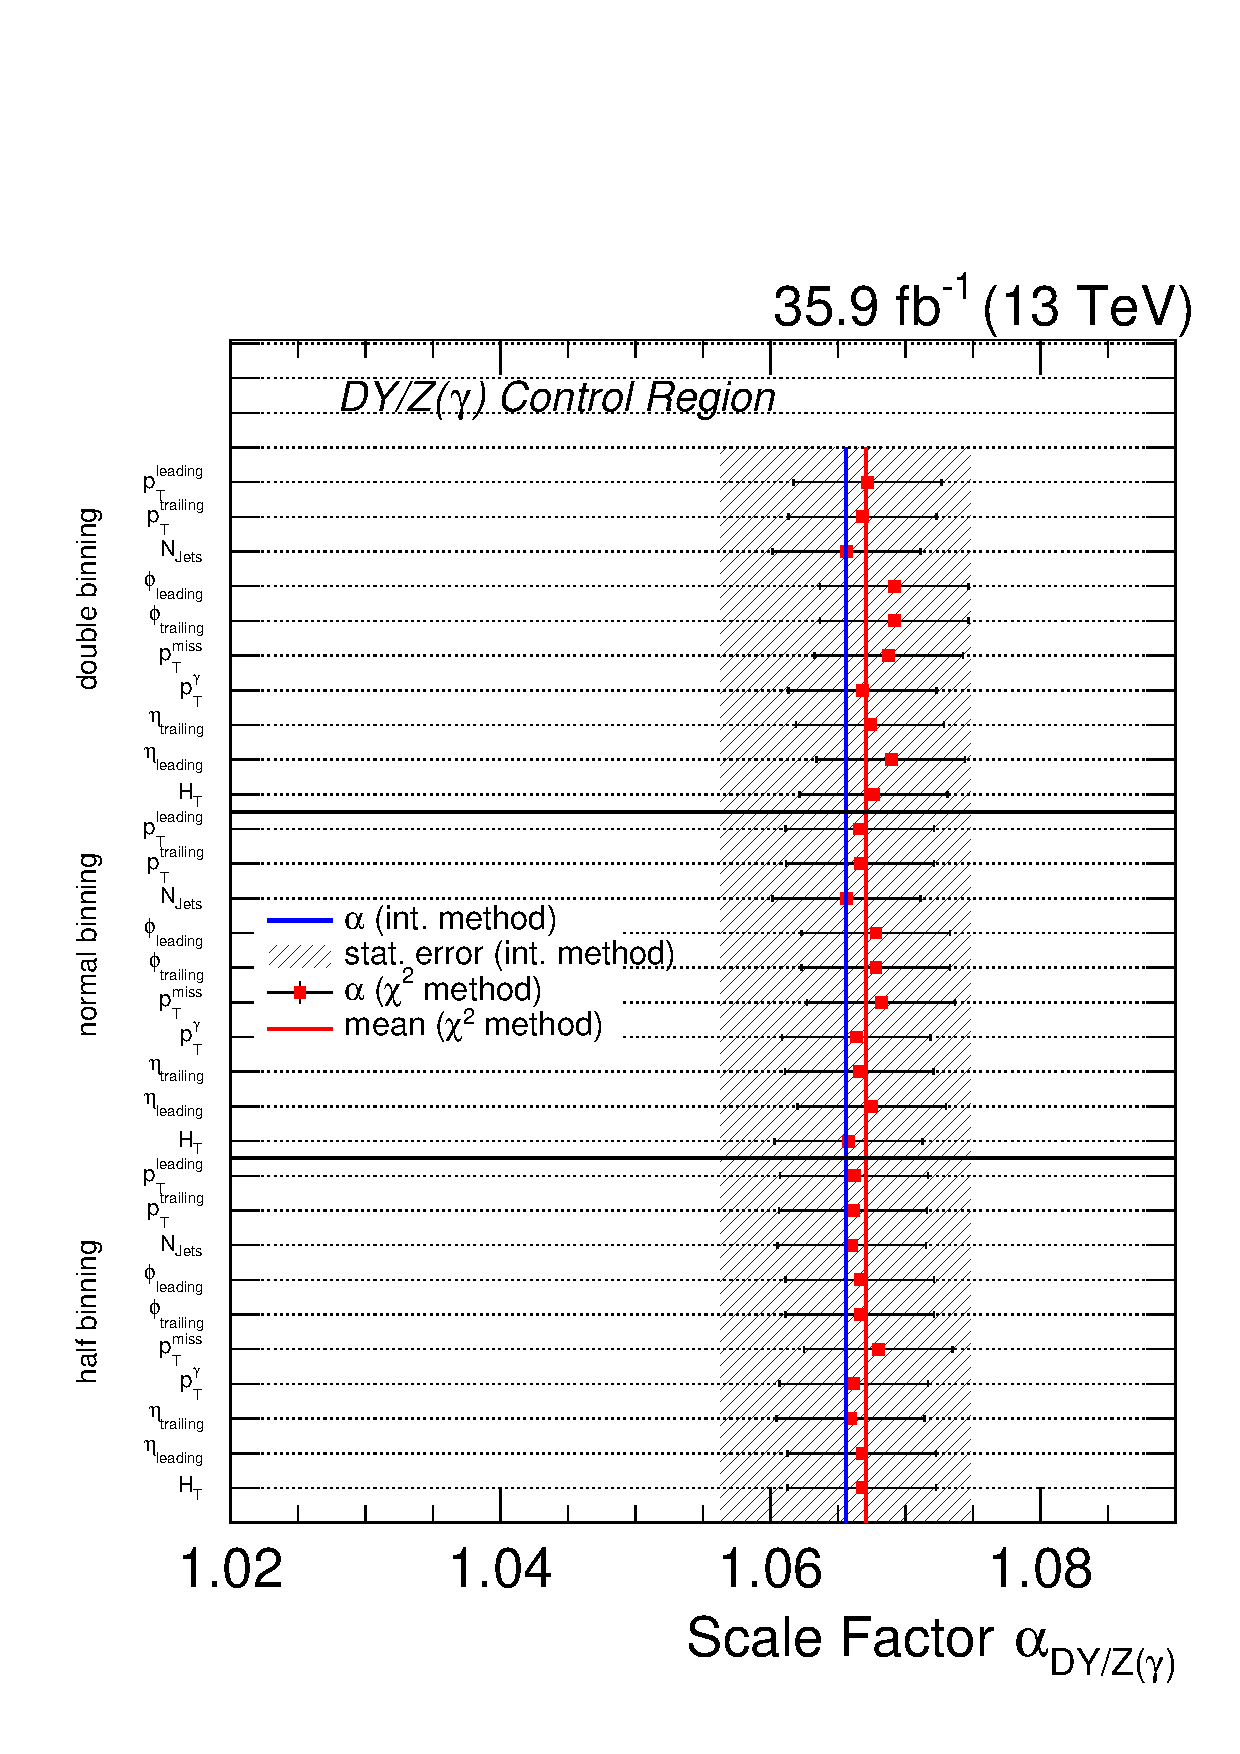
\includegraphics[width=\pairwidth]{figures/plots_CR/chi/DY_CompareLL}
 \caption{Example $\chi^2$-fit in the DY/$\PZ(\PGg)$ CR in the $\ptmiss$ distribution (left) with the polynomial fit. All fit results compared with the SF obtained from the integral method in different binnings and variables (right).}
 \label{fig:chiDY}
\end{figure}



\subsection{Other standard model backgrounds}
Additional minor backgrounds, such as $\PW\PZ\PGg$, $\PW\PW\PGg$, $\PW\PW$, and $\PW\PGg$ production, the production of $\PW$ bosons in association with jets, and single top processes as listed in \refTab{tab:MCsamples}, are taken from plain simulation after reweighting them as described in \refSec{sec:Simulation} to the measured luminosity and NLO and NNLO cross sections.

\FloatBarrier
\subsection{Validation of the background estimation}\label{sec:Validation}
After all main backgrounds are estimated using the corresponding CRs where the SFs are determined, the background prediction is validated in the VR defined in \refSec{sec:VR}. The VR is orthogonal to the SR while being not signal sensitive and kinematically similiar to the SR. Therefore, the VR is ideal to study the obtained background prediction.\\
Resulting comparisons between prediction and observed data in different distributions are shown in \refFig{fig:VR1} for the most important variables, such as $\ptmiss$ and $\mtTwo$, together with $\pt$ distributions of the leading and trailing lepton. Comparisons for the photon $\pt$ and the invariant dilepton mass $m_{\ell\ell}$ distributions are shown in \refFig{fig:VR2}.\\
Overall, the agreement is good in all distributions, although being limited by the low statistics in some kinematic regions. Kolmogorov-Smirnov tests are performed to gain more trust in the background prediction. As can be read from the resulting KS-values, each quoted on the corresponding plot, the predicted and observed shapes agree well considering statistical uncertainties and systematic uncertainties. Here, the shown systematic uncertainty originates merely from the statistical ones from the integral method. With $97$ data events measured and $93.9$ predicted, als the total number of events match between prediction and data.\\
Therefore, the background are assumed to be well predicted in the SR due to the similar kinematics in the VR based on the design as a kinematic sideband in $\ptmiss$ and $\mtTwo$.
\begin{figure}[tbp]
 \centering
 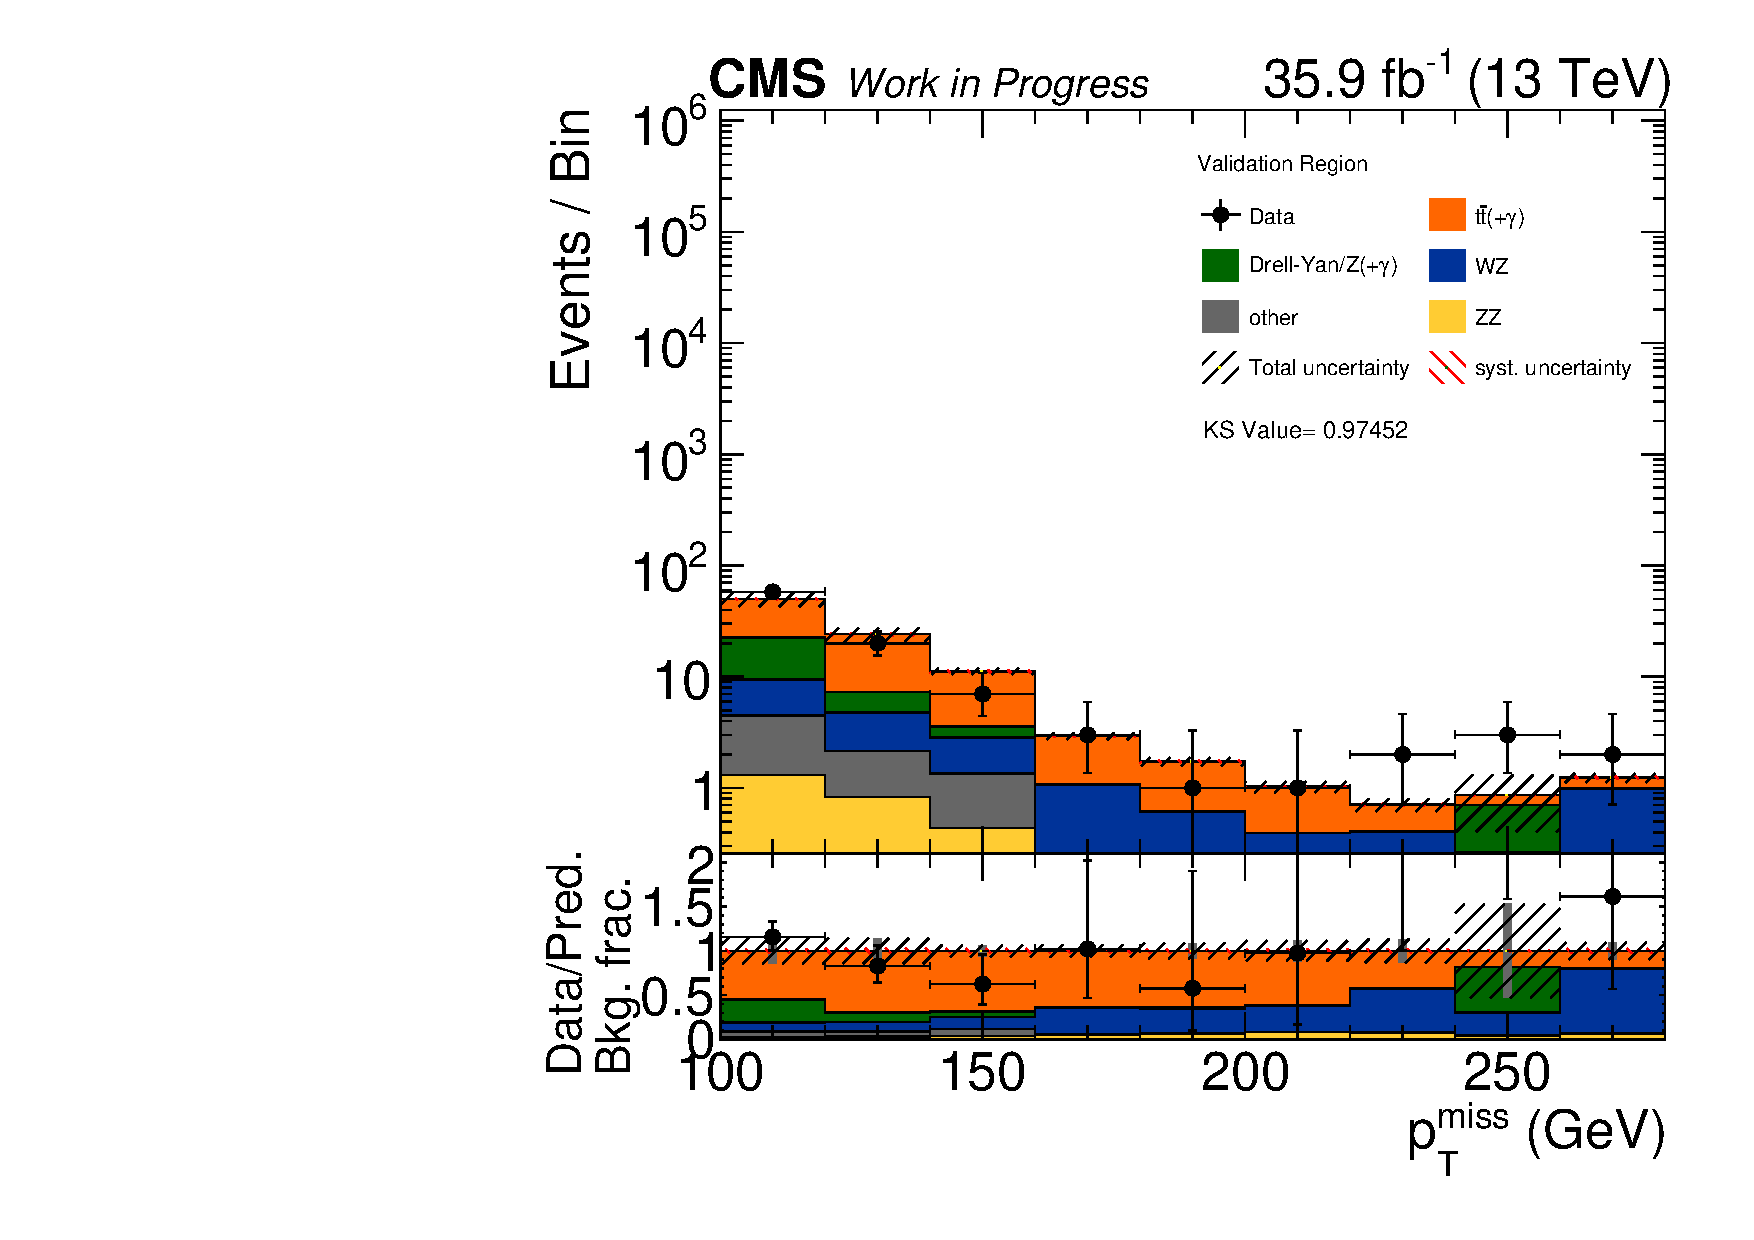
\includegraphics[width=\pairwidth]{figures/plots_VR/VR_LL_met_log}
 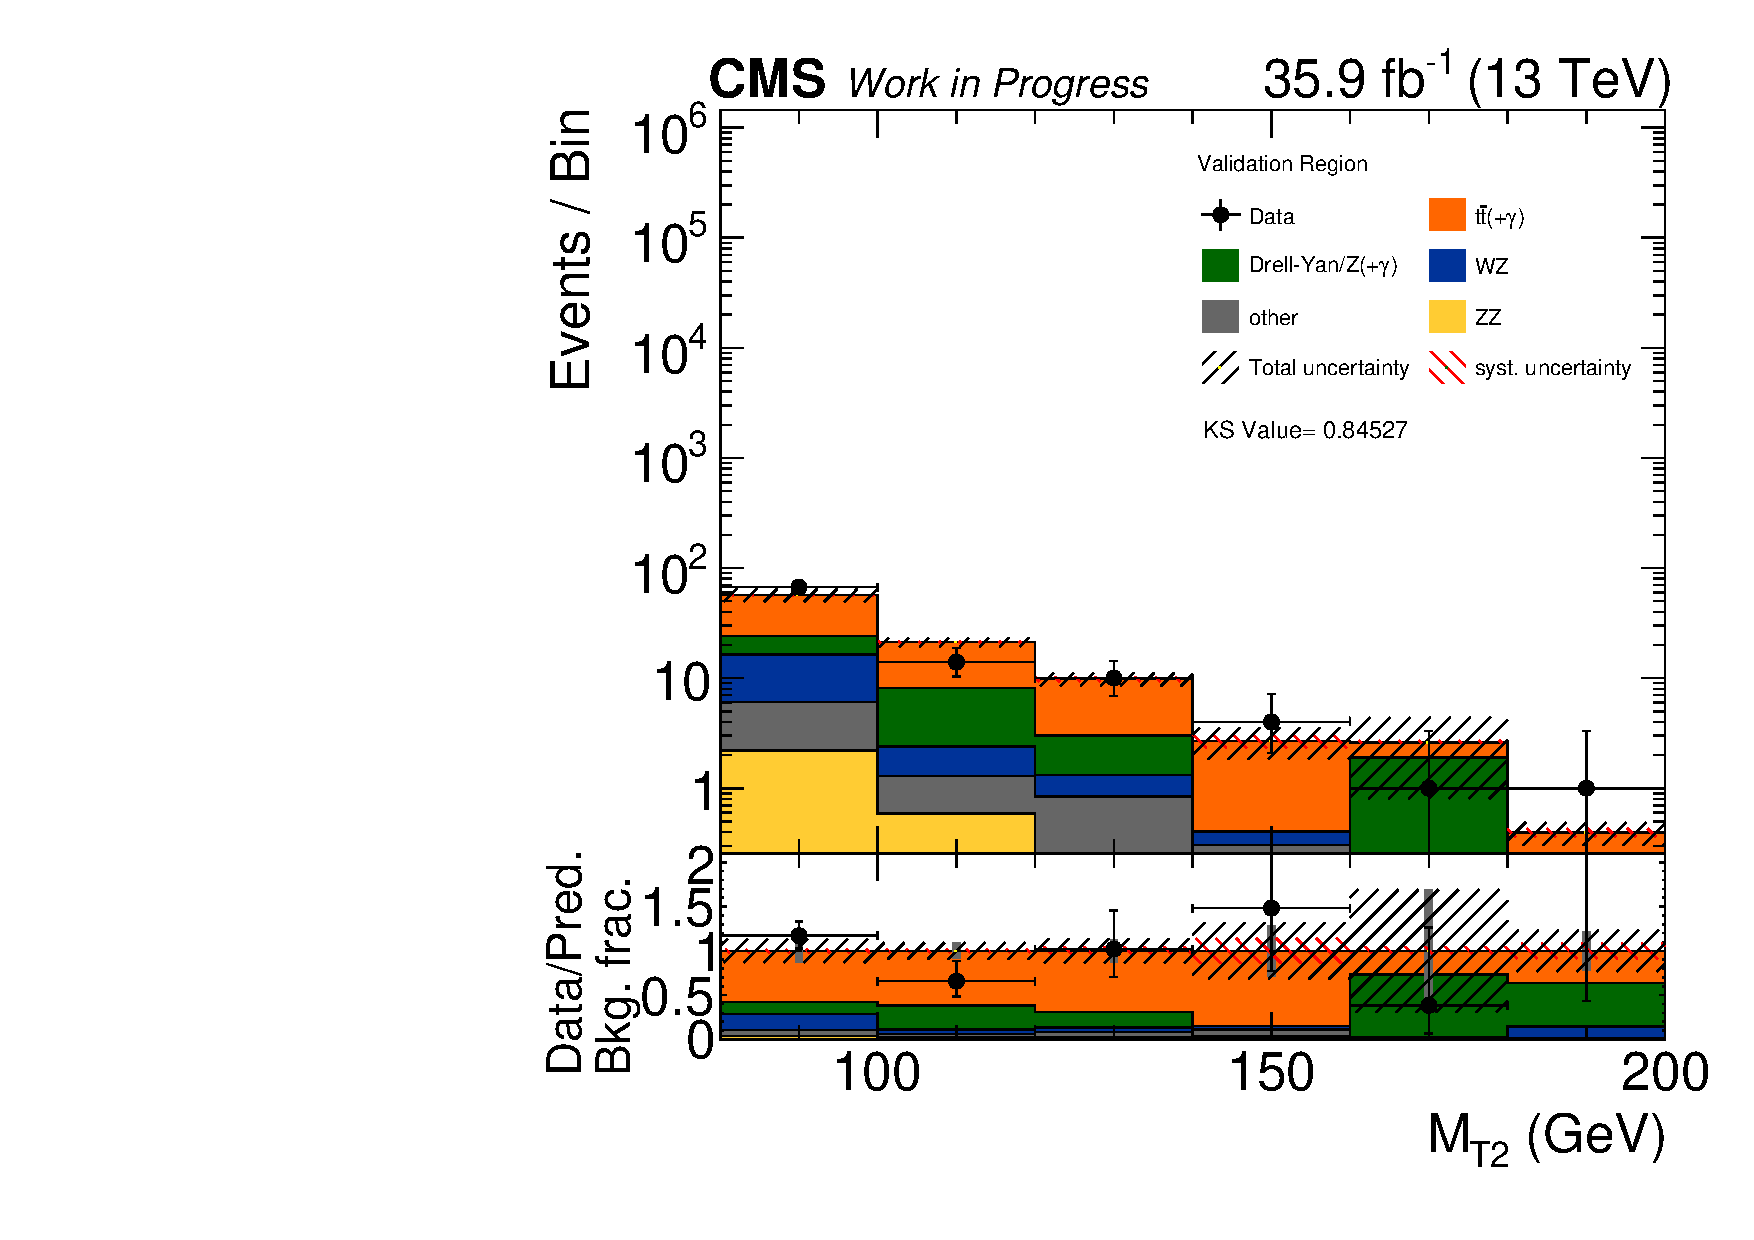
\includegraphics[width=\pairwidth]{figures/plots_VR/VR_LL_mt2_log}\\
 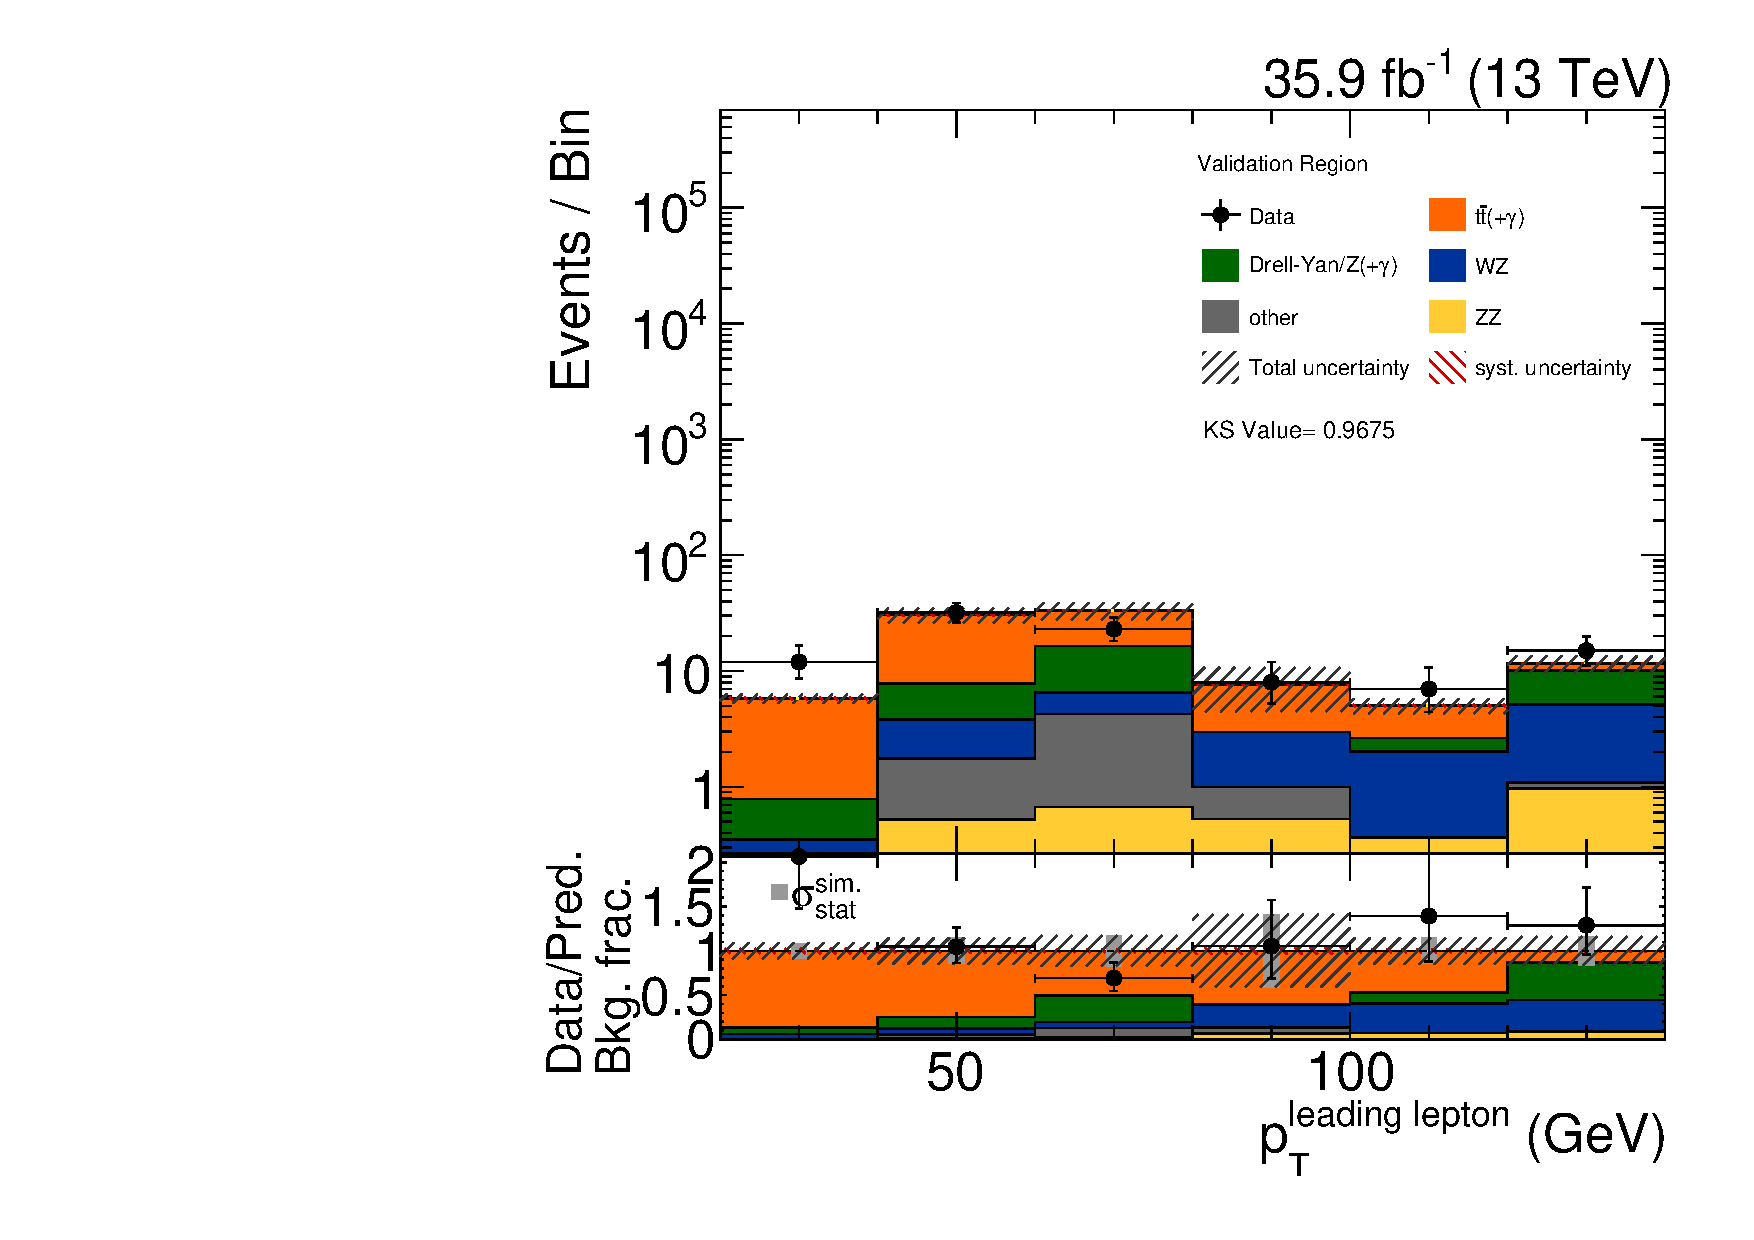
\includegraphics[width=\pairwidth]{figures/plots_VR/VR_LL_pt1_log}
 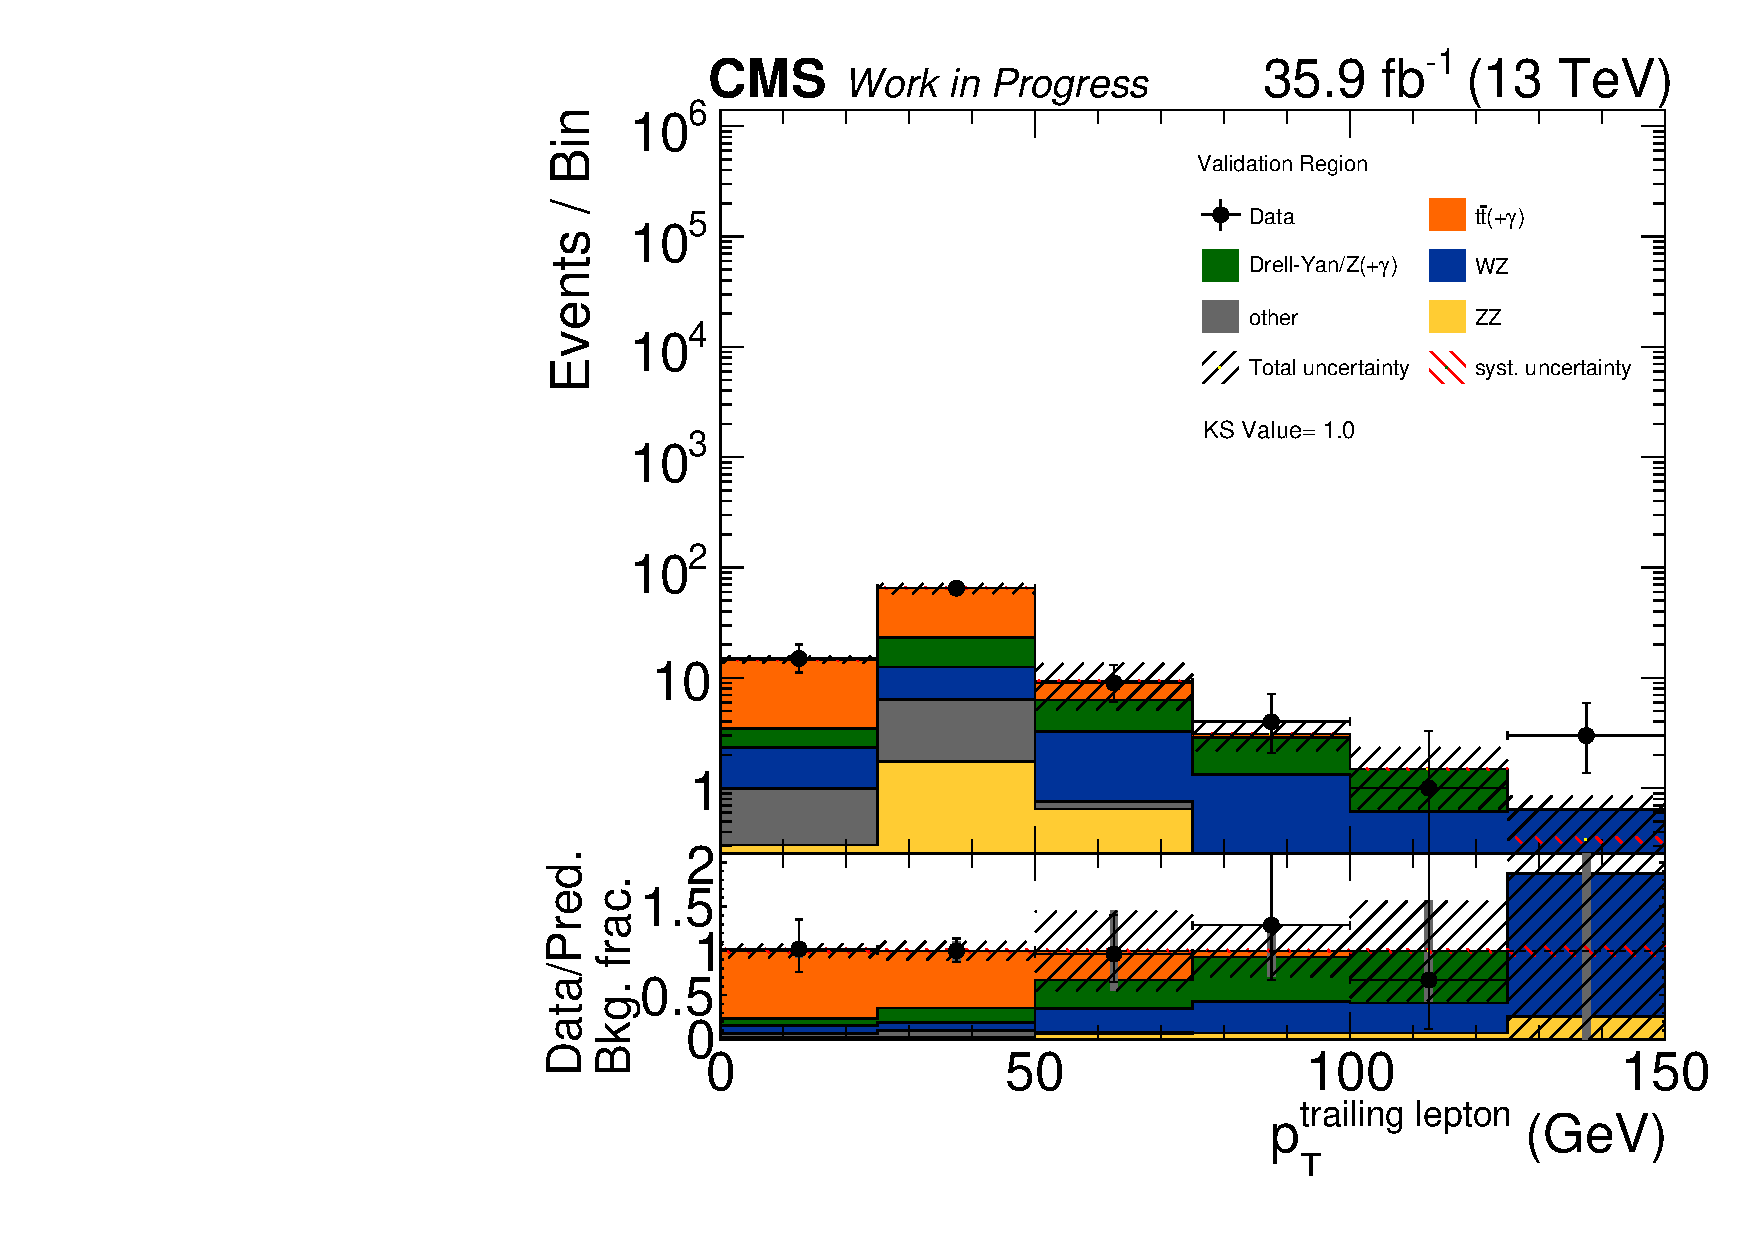
\includegraphics[width=\pairwidth]{figures/plots_VR/VR_LL_pt2_log}
 \caption{Comparisons between data and rescaled simulation in the VR in the $\ptmiss$, $\mtTwo$, and lepton $\pt$ distributions. Below each distribution, a ratio between data and prediction is shown. The uncertainty bands correspond to the systematic (red) and total uncertainty (gray). In addition, in the ratio plot the relative composition of the backgrounds is visualized. KS-values for the performed Kolmogorov-Smirnov test and the selection purity are also quoted.}
 \label{fig:VR1}
\end{figure}


\begin{figure}[tbp]
 \centering
 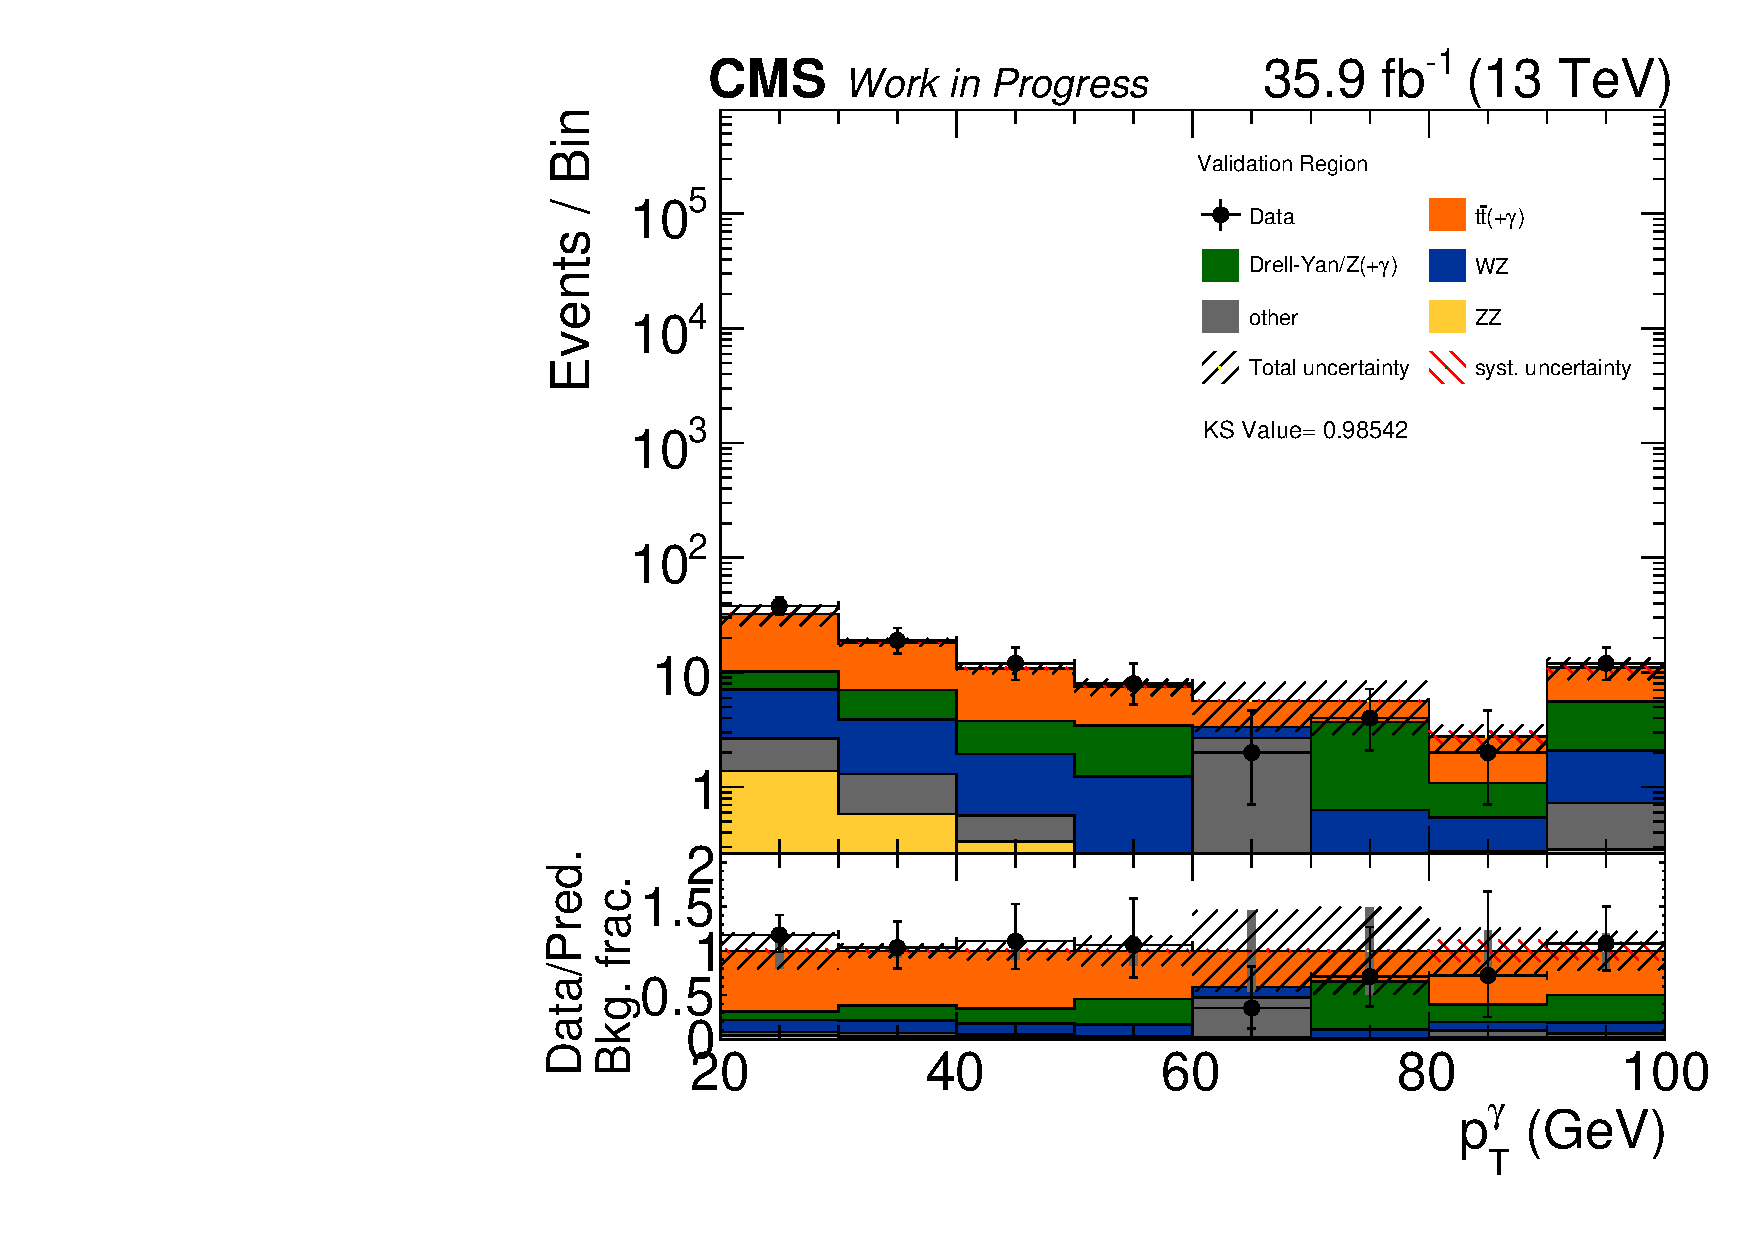
\includegraphics[width=\pairwidth]{figures/plots_VR/VR_LL_pt_g1_log}
 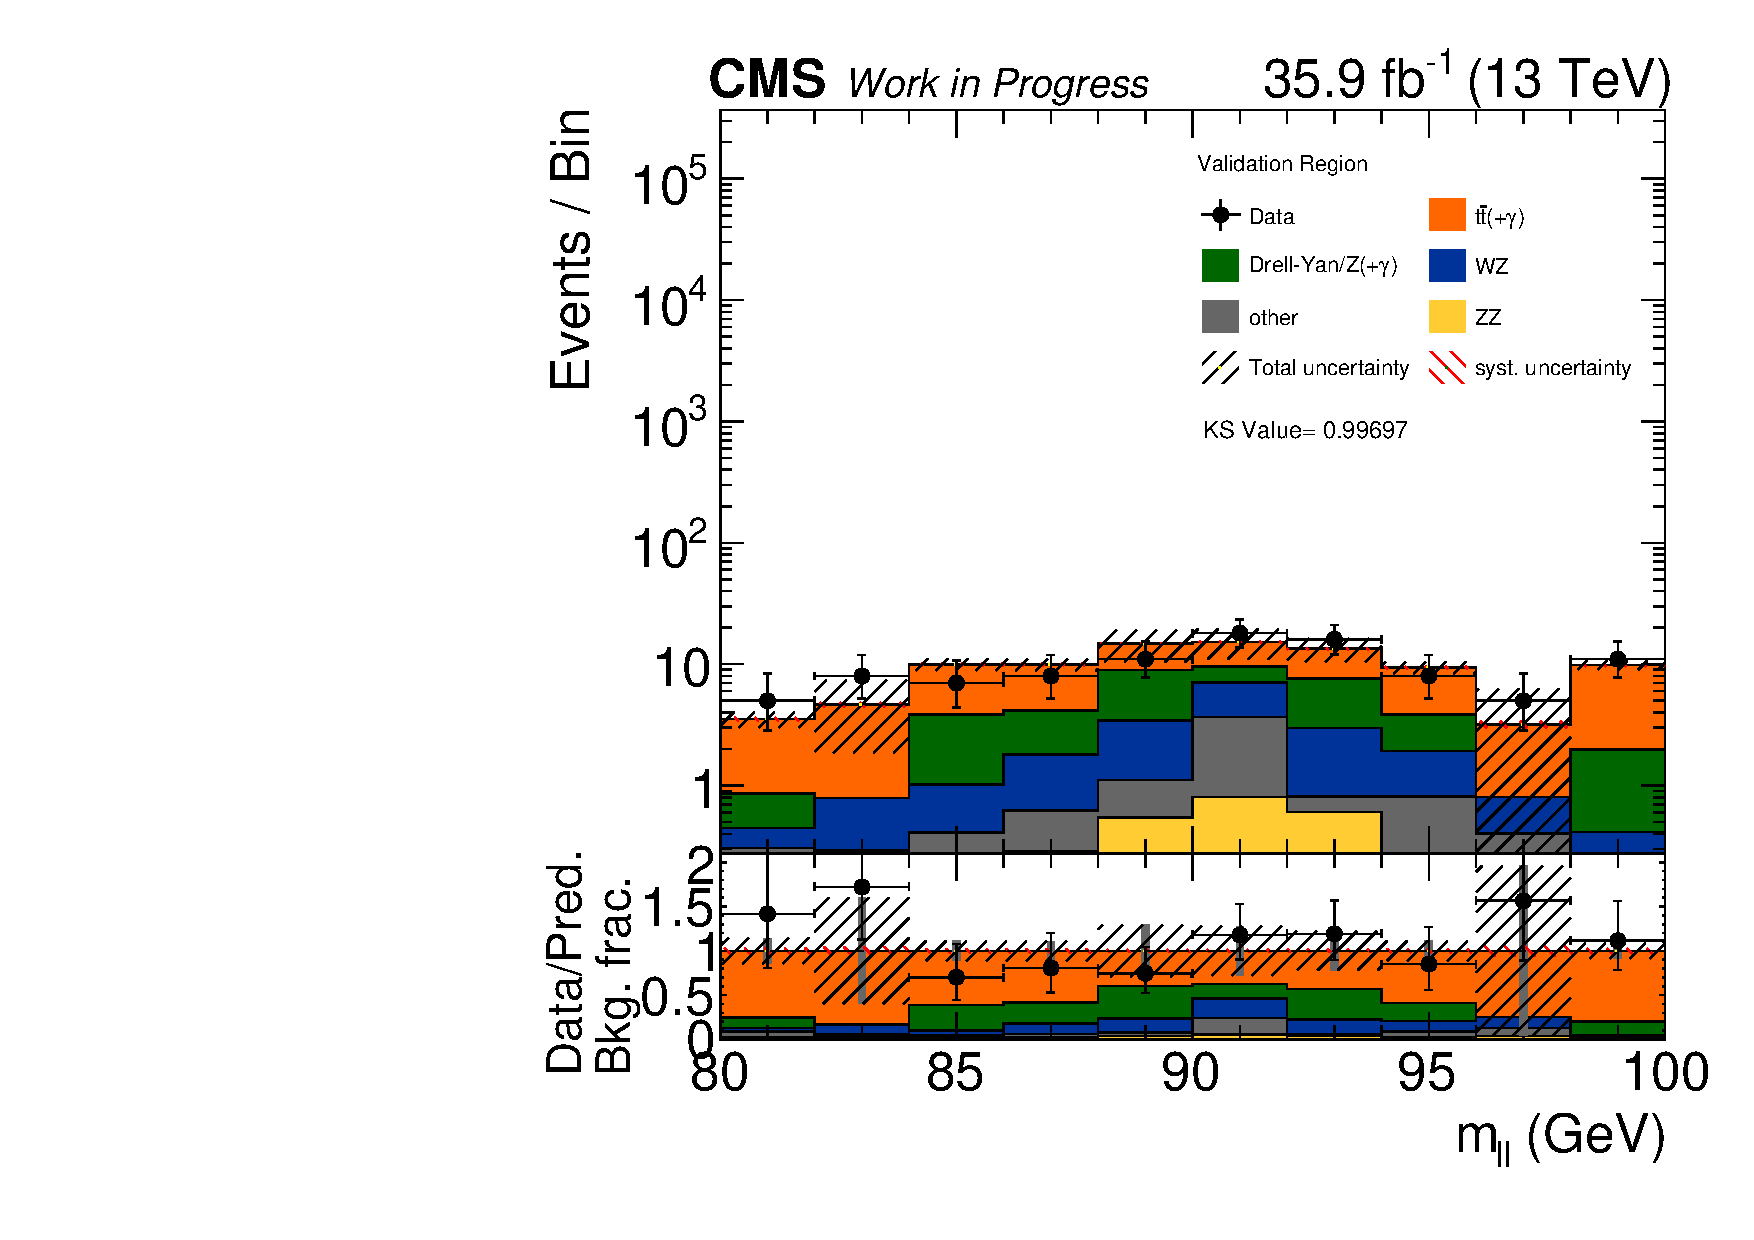
\includegraphics[width=\pairwidth]{figures/plots_VR/VR_LL_m_ll_log}
 \caption{Comparisons between data and rescaled simulation in the VR in the photon $\pt$ and invariant dilepton mass distribution. Below each distribution, a ratio between data and prediction is shown. The uncertainty bands correspond to the systematic (red) and total uncertainty (gray). In addition, in the ratio plot the relative composition of the backgrounds is visualized. KS-values for the performed Kolmogorov-Smirnov test are also quoted.}
 \label{fig:VR2}
\end{figure}


\subsection{Signal contamination}\label{sec:signalCont}
If SUSY was realized in nature, it would not only produce events in the SR, but also some of them may appear in the CRs that are used to determine a proper background prediction. To account for this effect, the so-called signal contamination of the background CRs is not considered in the background estimation itself, but is translated into a reduction of the predicted signal yield in the SR. Hence, the signal contamination needs to be measured for each signal point of all samples individually in all CRs.\\
Therefore, the fraction of expected signal events relative to the total number of background events in each CR is measured. Examples for the contamination of the \texttt{TChiZG} SMS in the DY/$\PZ(\PGg)$ CR and the GMSB model in the $\PW\PZ$ CR are shown in \refFig{fig:signalCont}, because they are the largest ones observed. As can be seen, the contributions of signal events are mainly negligible, although the signal contamination reaches around $3\%$ for very low bino and wino masses in the GMSB model.\\
To account for those effects, these relative fractions are used to lower the signal expectation in each SR bin individually. If $\rho$ is the fraction of signal events in the CR, in each SR bin the absolute signal event yield reduced with the following formula
\begin{equation}
 \#signal_{after} = \#signal_{before} - \rho\cdot\#background,
\end{equation}
where $\#signal_{before}$ and $\#signal_{after}$ are the total number of signal events per bin before and after the correction, and $\#background$ is the number of predicted background events in this bin.

\begin{figure}
 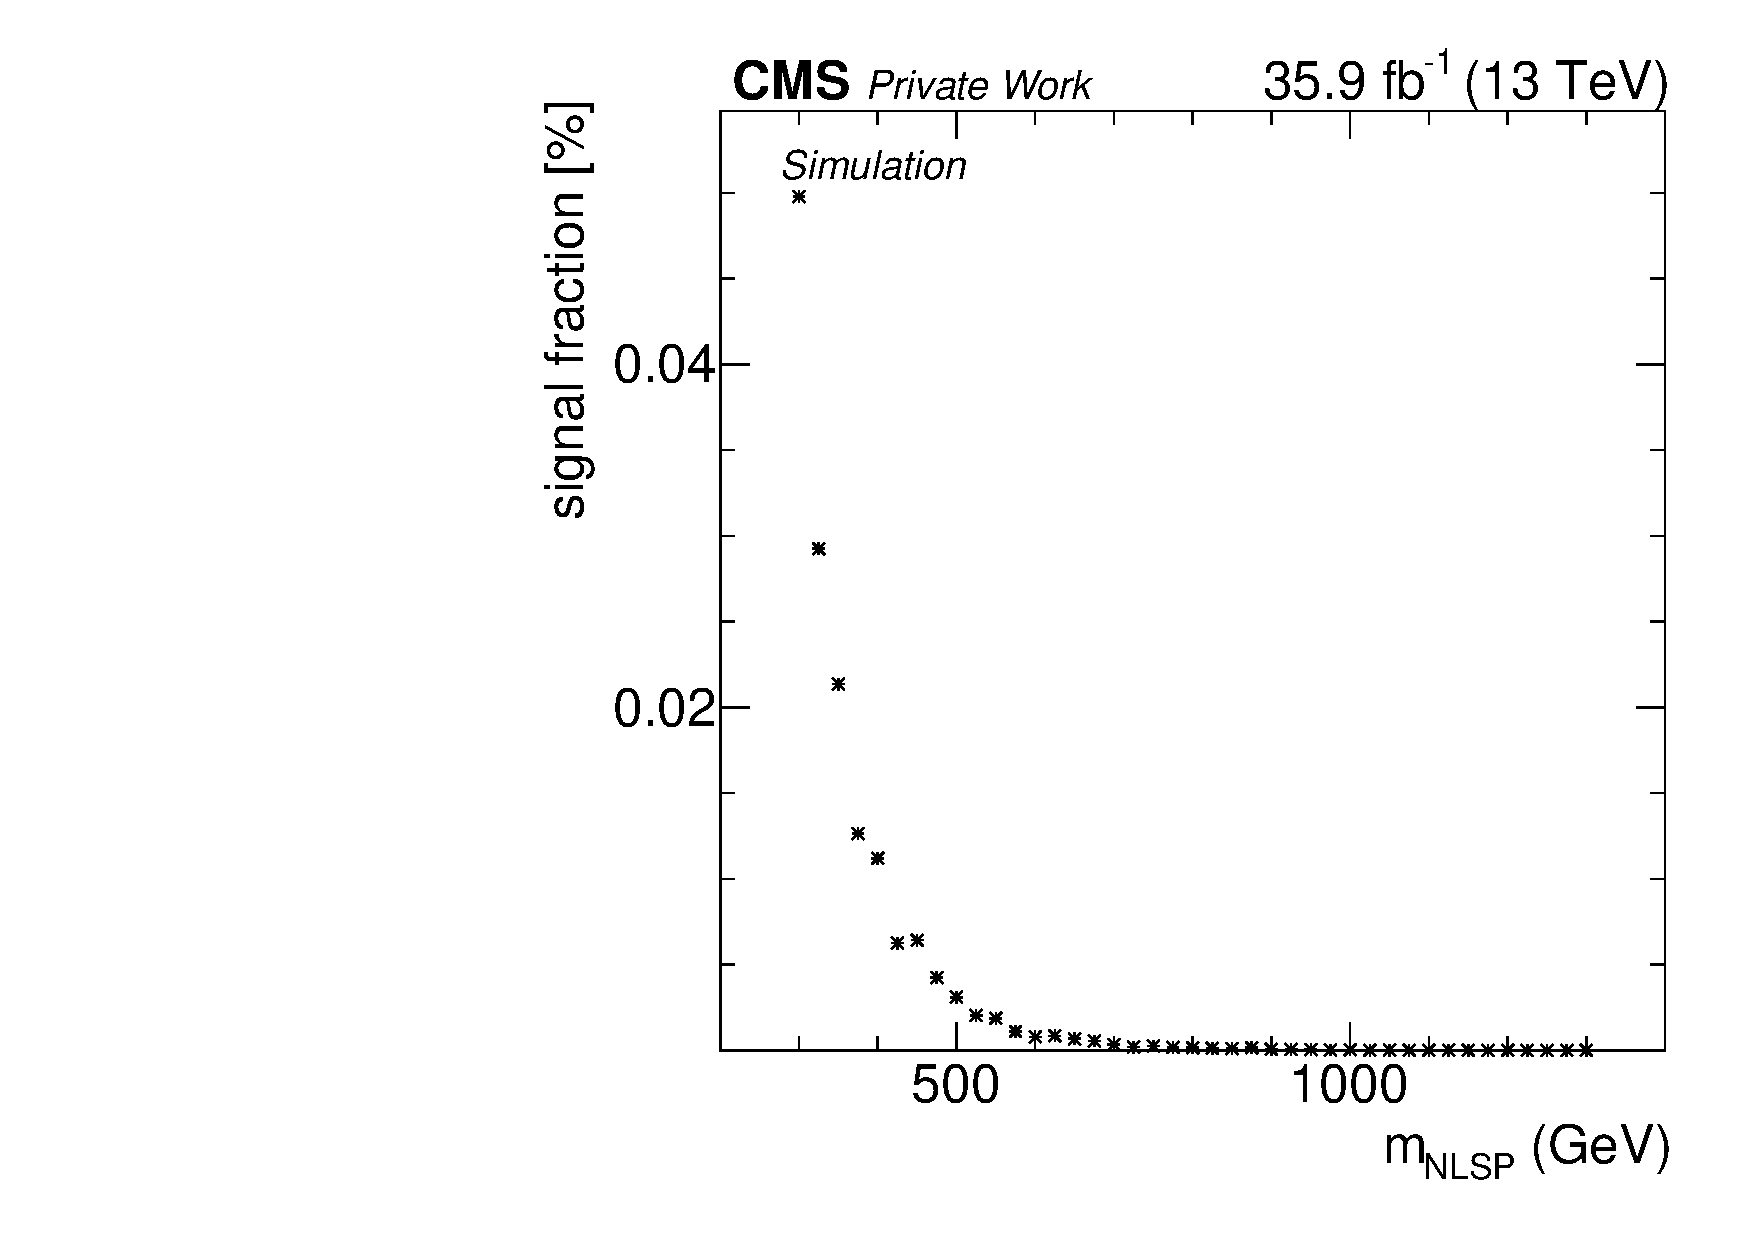
\includegraphics[width=\pairwidth]{figures/contamination/tching_DY}
 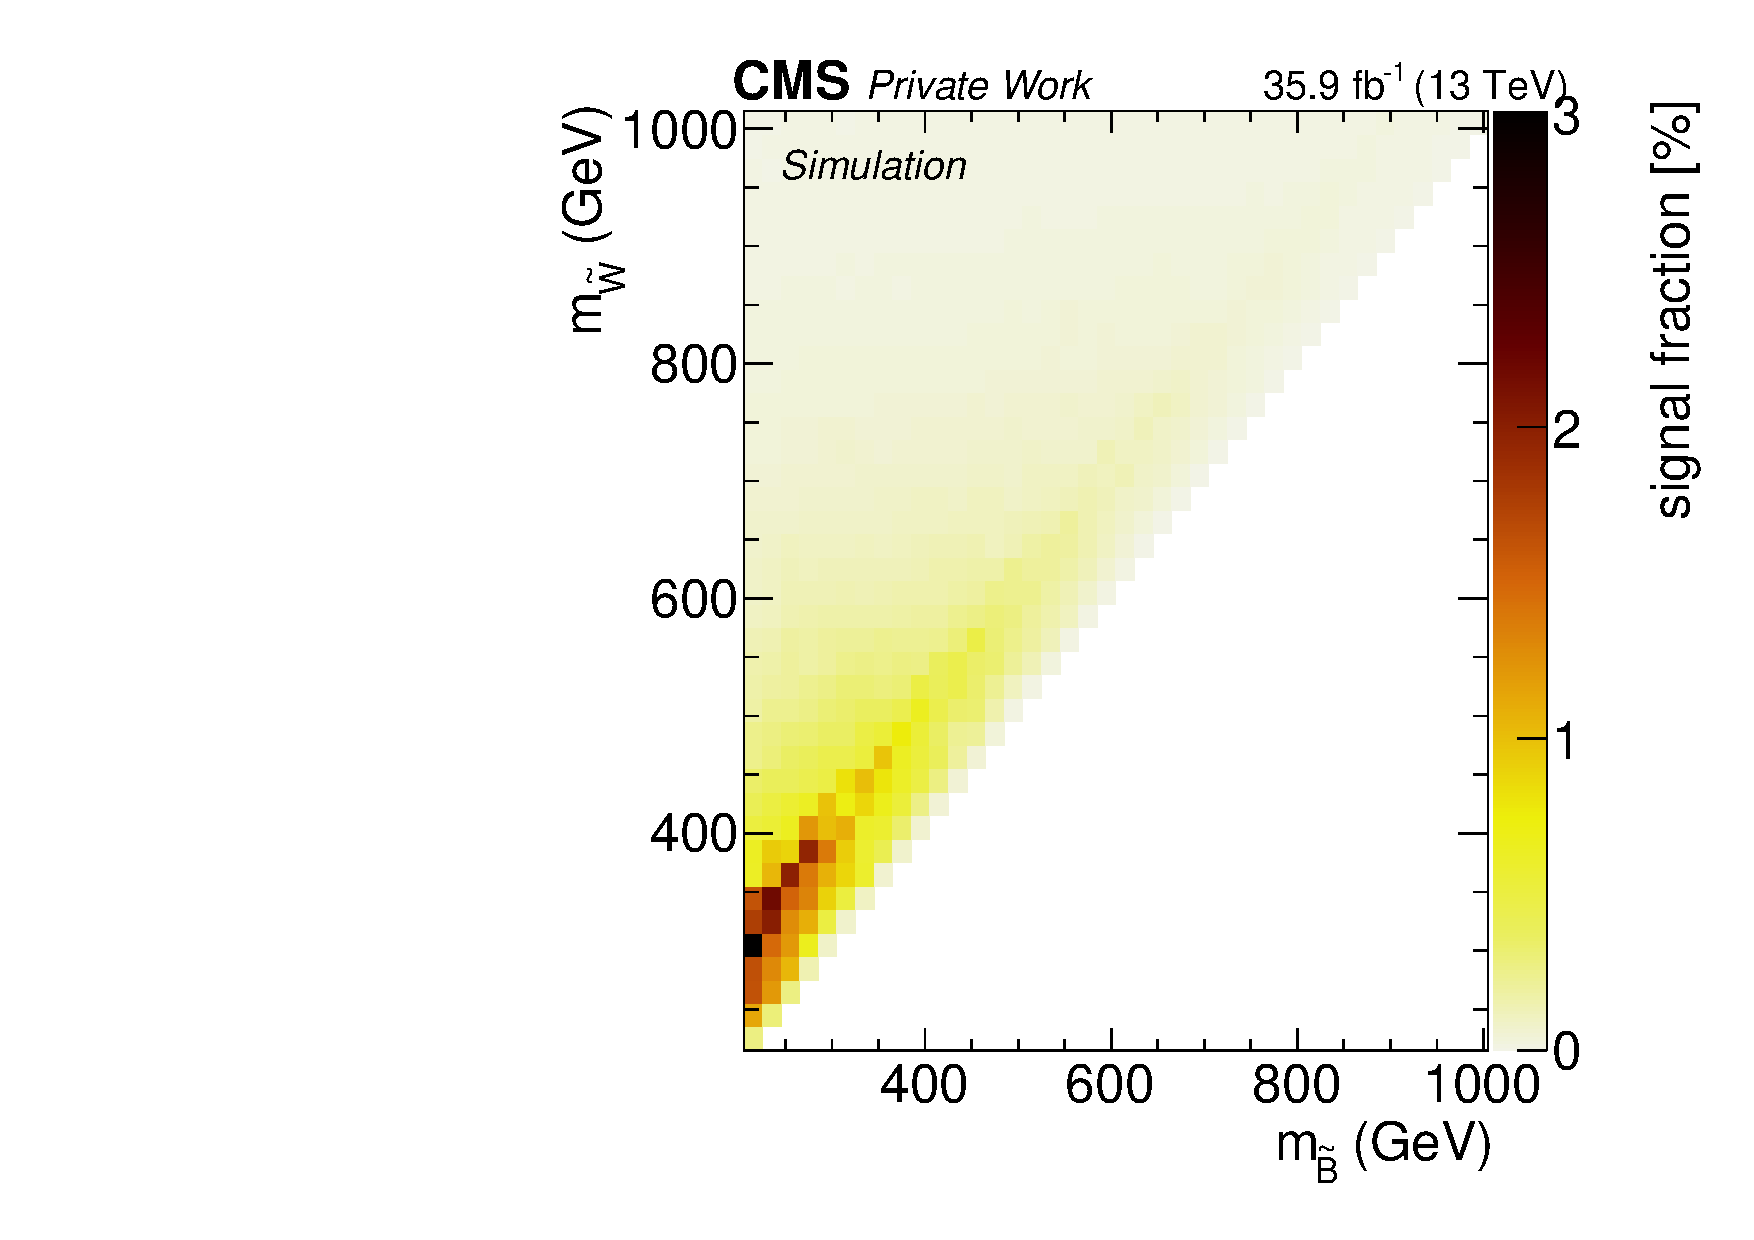
\includegraphics[width=\pairwidth]{figures/contamination/gmsb_WZ}
 \caption{Signal fraction compared to the total background event yield for different signal points of the \texttt{TChiZG} in the DY/$\PZ(\PGg)$ CR (left) and the GMSB model in the $\PW\PZ$ CR (right).}
 \label{fig:signalCont}
\end{figure}
In total, the influence of signal contamination to the final result is rather negligible, because for most of the signal points the contributions to all CRs are very low. In cases where they exceed the level of a few percent, their influence will not matter in the final interpretation, since for those low SUSY mass signal points, the expectation for the signal yield in the SR is sufficiently high.


\section{Study of systematic uncertainties}\label{sec:Syst}
In addition to the statistical uncertainties arising from the background prediction method itself, various systematic effects and their impact on the final prediction need to be evaluated.

\subsection{Background uncertainties}
Systematic uncertainties arise from the data pileup distribution, which is used to rescale the simulated samples as explained in \refSec{sec:Simulation}, the measurement of the total integrated luminosity, the measurement of the jet energy scale (JES) and the jet energy resolution (JER), the measured trigger efficiencies as discussed in \refSec{sec:triggEff}, corrections for a different photon and lepton reconstruction efficiency in simulation and data, the PDF sets used in the simulation process, and choice of the factorization scale and renormalization scale.\\
These measurements and underlying effects all contribute systematic uncertainties on the final background prediction. Cross section, trigger, and luminosity uncertainties cancel for the four main background contributions due to the integral method, but are relevant for the other minor contributions. For these a cross section uncertainty of $50\%$ is assigned to the final yield to account for  differences between cross section measurement and theoretical prediction, and to consider the circumstance, that only a special phase space region is investitaged in the analysis.\\
The uncertainty on the luminosity measurement with $2.5\%$~\cite{LumiUncert} and the uncertainty on the trigger efficiency, that is estimated to be $3\%$ (see \refSec{sec:triggEff}), propagate directly to the final prediction.\\
All other uncertainties are uncertainties in the shapes of the predicted spectra, and need to be determined in another way. In order to estimate the impact of the JES and JER, the pileup reweighting, and the lepton and photon identification and reconstruction corrections, the background prediction is performed again with the underlying quantities shifted one standard deviation up and down. Hence, two additional predictions for each SR bin are obtained, and half of the difference between those, relative to the nominal prediction, is taken as the corresponding systematic uncertainty.\\
The uncertainty arising from the JES (JER) is observed to be around $1-6.5\%$ ($0.2-16.1\%$) for the four main backgrounds, while uncertainty arising from the lepton (photon) identification and reconstruction is $1.8-3.2$ ($0.7-1.5\%$). The uncertainty due to pileup reweighting varies between $0.2\%$ and $5\%$ for these four backgrounds. For the other backgrounds the uncertainties are higher, but the absolute effect is negligible compared to the other background controbutions due to the low predicted event yields.
To estimate the effect on the choice of the renormalization scale $\mu_R$ and factorization scale $\mu_F$, these two are varied in combinations of the factors $0.5$, $1$, and $2$, and eight new background predictions are obtained. The half of the difference between the two outliers, relative to the nominal prediction, is chosen as the systematic uncertainty. It varies between $21.-22.5\%$ for all backgrounds over all bins.\\
To determine the systematic uncertainty arising from the used PDF sets, one hundred different PDF variations are studied, and for each the background prediction method is performed again, thus one hundred different predictions for the SR are obtained. From this distribution of predicted yields, the standard deviation and the mean can be calculated. The standard deviation with respect to the mean is considered as the systematic uncertainty, and varies between $0.8\%$ and $3.3\%$ for all backgrounds and bins.\\
The uncertainty arising from the choice of order regarding the four SFs determined in the CRs, is estimated by testing all $4!=24$ possibilities, and calculating the largest deviation from the nominal SFs. This envelope is considered as a systematic uncertainty on the SFs on top of the statistical uncertainty. Both uncertainties are added quadratically, such that one final uncertainty for each SF is obtained.
\refTab{tab:systuncBKG} lists ranges for all final systematic uncertainties for all backgrounds individually.
\begin{table}[tbp]
 \centering
 \caption{Systematic uncertainty ranges for all background predictions in the signal region.}
 \small
 \label{tab:systuncBKG}
 \begin{tabular}[width=\textwidth]{llllll}
                            & $tt(\PGg)$  & DY/Z$(\PGg)$  & $\PW\PZ$    & $\PZ\PZ$    & Other       \\\hline
  PDF                       & $0.8-1.5\%$ & $2.6-3.3\%$   & $0.5-0.7\%$ & $2.2-2.4\%$ & $1.1-1.2\%$ \\
  Renorm. and fact. scale   & $3.3-7.1\%$ & $18.2-22.5\%$ & $4-6\%$     & $3.7-4.1\%$ & $2.1-9.3\%$ \\
  Jet energy scale          & $4.6-6.5\%$ & $4.4-5\%$     & $2.8-4.8\%$ & $1-1.9\%$   & $0-50.7\%$  \\
  Jet energy resolution     & $1.6-3.1\%$ & $0.7-16.1\%$  & $1-1.8\%$   & $0.2-1.4\%$ & $0-50.7\%$  \\
  Lepton ID and reco.       & $2.8-2.9\%$ & $2.2-3.4\%$   & $3.3\%$     & $1.8\%$     & $4.2\%$     \\
  Photon ID and reco.       & $0.7-0.8\%$ & $1.4-1.5\%$   & $1-1.1\%$   & $0.9\%$     & $0.7-1.9\%$ \\
  Luminosity                & -           & -             & -           & -           & $2.5\%$     \\
  Pileup                    & $1.2-2\%$   & $1-5\%$       & $0.2-2.5\%$ & $1.5-1.7\%$ & $0.1-10\%$  \\
  Trigger efficiency        & -           & -             & -           & -           & $3\%$       \\
  Scale factor $\alpha_{i}$ & $4.1\%$     & $0.9\%$       & $3.9\%$     & $5.7\%$     & -           \\
  Cross section             & -           & -             & -           & -           & $50\%$      \\
  \hline
 \end{tabular}
\end{table}
Besides uncertainties for some backgrounds, such as DY/$\PZ(\PGg)$ and the other composed backgrounds, exceed the level of $10\%$, where statistical fluctuations based on changes of different quantities play an important role, all other systematic uncertainties are of the order of a few percent. This reflects the stability and robustness, that was observed in the scale factor determination itself.


\subsection{Signal uncertainties}
Signal uncertainties need to be studied in order to interpret the results statistically in each SUSY model.
Most of the signal uncertainty determination methods behave the same as for the backgrounds, but some additional effects need to be considered. Some calculations change, since the detector response in the signal MC simulation was performed using the \FASTSIM package.\\
For the determination of the pileup uncertainty, a different method is applied. The pileup distribution is split into a low PU ($N_{vertices}<20$) and a high PU ($N_{vertices}>20$) region, and the difference in the total signal acceptance is determined. Half of this difference is treated as the systematic uncertainty.\\
Because the modeling of the $\ptmiss$ distribution is very complicated, and in the \FASTSIM package only a simplified detector response is parameterized, the difference between generated $\ptmiss$ and reconstructed $\ptmiss$ is investigated. Thus, the whole analysis is reperformed for the signal, where the reconstructed $\ptmiss$ is replaced with the generated $\ptmiss$ for each event, and the difference in the acceptance is examined. Half of the deviation is taken as the systematic uncertainty.\\
For the signal simulation, no PDF uncertainties are available. The initial state radiation dependent reweightings mentioned in \refSec{sec:Simulation} introduce systematic effects on the signal yield expectation. Therefore, the same method as mentioned above for the identification and reconstruction uncertainties on the background prediction is performed.\\
Ranges for all signal uncertainties including the statistical one are given in \refTab{tab:systuncSignal} altogether for all signal models considered in the analysis.\\
All other systematic effects, except for the luminosity uncertainty and the uncertainty arising from the trigger efficiency measurement are correlated with the statistical uncertainty.
Hence, large ranges are observable due to the limited statistics that is available for each signal point. This is due to time and resource saving reasons, since a large number of different signal points is being generated. In addition, the low available number of signal events becomes much lower, as only leptonic decay branches of the Z boson are considered and its branching fraction ($\mathcal{BR}(\PZ\to\ell^+\ell^-)\approx3.36\%$~\cite{PDG}) is very low. Nevertheless, in most of the relevant signal points the uncertainties do not exceed the level of a few percent.
\begin{table}[tbp]
 \centering
 \caption{Ranges for all the systematic uncertainties for all signal models.}
 \normalsize
 \label{tab:systuncSignal}
 \begin{tabular}[width=\textwidth]{ll}
  Uncertainty                   & Range $[\%]$ \\\hline
  Statistical                   & $3.2-85$     \\
  Luminosity                    & $2.6$        \\
  Pileup                        & $<0.1-143$   \\
  Jet energy scale              & $<0.1-62$    \\
  Jet energy resolution         & $<0.1-63$    \\
  Trigger Efficiency            & $3$          \\
  Lepton ID and reconstruction  & $<0.1-5.6$   \\
  Photon ID and reconstruction  & $1.4-1.5$    \\
  \FASTSIM uncert. in $\ptmiss$ & $<0.1-293$   \\
  ISR reweighting               & $<0.1-11$    \\
  Renorm. and fact. scale       & $0.1-11$     \\
  \hline
 \end{tabular}
\end{table}
